\documentclass[12pt,a4paper,oneside]{report}

% --- Ngôn ngữ và font chữ ---
\usepackage[utf8]{inputenc}
\usepackage[T5]{fontenc}
\usepackage[vietnamese]{babel}
\usepackage{mathptmx} % Font Times New Roman tương thích pdfLaTeX

% --- Định dạng trang và căn lề ---
\usepackage[left=3cm,right=2cm,top=2.5cm,bottom=2.5cm]{geometry}
\usepackage{setspace}
\setstretch{1.3} % Giãn dòng 1.3 theo quy định BTL
\setlength{\emergencystretch}{3em}
\setlength{\parindent}{1cm}
\setlength{\parskip}{2pt}

% --- Định dạng danh sách và khoảng cách float ---
\usepackage{enumitem}
\setlist{itemsep=1pt, topsep=2pt, parsep=0pt, partopsep=0pt}
\setlength{\textfloatsep}{7pt plus 2pt minus 2pt}
\setlength{\floatsep}{5pt plus 2pt minus 2pt}
\setlength{\intextsep}{6pt plus 2pt minus 2pt}
\renewcommand{\topfraction}{0.92}
\renewcommand{\bottomfraction}{0.88}
\renewcommand{\textfraction}{0.08}
\renewcommand{\floatpagefraction}{0.8}

% --- Định dạng tiêu đề chương và Heading 1 ---
\usepackage{titlesec}
\titleformat{\chapter}[block]
  {\normalfont\LARGE\bfseries\centering}
  {\chaptertitlename\ \thechapter:}
  {0.5em}
  {}
\titleformat{name=\chapter,numberless}[block]
  {\normalfont\LARGE\bfseries\centering}
  {}
  {0pt}
  {}
\titlespacing*{\chapter}{0pt}{-20pt}{10pt}
\titlespacing*{\section}{0pt}{8pt}{3pt}
\titlespacing*{\subsection}{0pt}{5pt}{2pt}
\usepackage{amsmath,amssymb,amsfonts,bm}
\numberwithin{equation}{chapter}
\AtBeginDocument{%
  \setlength{\abovedisplayskip}{4pt plus 2pt minus 2pt}%
  \setlength{\belowdisplayskip}{4pt plus 2pt minus 2pt}%
  \setlength{\abovedisplayshortskip}{2pt plus 1pt minus 1pt}%
  \setlength{\belowdisplayshortskip}{2pt plus 1pt minus 1pt}%
}

% --- Bảng biểu, hình ảnh và chú thích ---
\usepackage{graphicx}
\usepackage{booktabs}
\usepackage{longtable}
\usepackage{array}
\usepackage{tabularx}
\usepackage{float}
\usepackage{subcaption}
\usepackage{caption}
\captionsetup[table]{position=top,skip=4pt,labelfont=bf,textfont=bf,font=small}
\captionsetup[figure]{position=bottom,skip=4pt,labelfont=it,textfont=it,font=small}
\numberwithin{figure}{chapter}
\numberwithin{table}{chapter}

% --- TikZ và đồ họa ---
\usepackage{tikz}
\usetikzlibrary{shapes.geometric, arrows.meta, positioning, calc}

% --- Trình bày mã nguồn & Giả mã ---
\usepackage{listings}
\usepackage{algorithm}
\usepackage{algorithmic}
\floatname{algorithm}{Thuật toán}
\lstset{
    basicstyle=\small\ttfamily,
    breaklines=true,
    numbers=left,
    numberstyle=\tiny,
    frame=single,
    tabsize=2,
    showstringspaces=false
}

% --- Liên kết và màu sắc ---
\usepackage{xcolor}
\usepackage{hyperref}
\hypersetup{
    colorlinks=true,
    linkcolor=blue!80!black,
    citecolor=blue!80!black,
    urlcolor=teal!80!black
}

% --- Mathematical Macros (latex_template standard) ---
\newcommand{\R}{\mathbb{R}}
\newcommand{\E}{\mathbb{E}}
\newcommand{\Var}{\mathrm{Var}}
\newcommand{\IoU}{\mathrm{IoU}}

\begin{document}

% ==================== PHẦN MỞ ĐẦU (FRONTMATTER) ====================
\pagenumbering{roman}

% 1. Trang bìa chính và trang phụ bìa
% Trang bìa chính
\begin{titlepage}
\begin{tikzpicture}[remember picture, overlay]
  % Viền ngoài
  \draw[line width = 2pt] 
    ($(current page.north west) + (2.5cm,-2.0cm)$) 
    rectangle 
    ($(current page.south east) + (-1.5cm,2.0cm)$);
  % Viền trong
  \draw[line width = 0.8pt] 
    ($(current page.north west) + (2.6cm,-2.1cm)$) 
    rectangle 
    ($(current page.south east) + (-1.6cm,2.1cm)$);
\end{tikzpicture}

\begin{center}
    \vspace*{-0.5cm}
    {\large \textbf{TRƯỜNG ĐẠI HỌC GIAO THÔNG VẬN TẢI}}\\[0.2cm]
    {\large \textbf{KHOA CÔNG NGHỆ THÔNG TIN}}\\[0.2cm]
    {\large \textbf{BỘ MÔN KHOA HỌC MÁY TÍNH}}\\[0.8cm]

    
\includegraphics[width=3.2cm]{figures/LogoUTC.jpg}\\[0.9cm]

    {\Large \textbf{BÁO CÁO BÀI TẬP LỚN}}\\[0.3cm]
    {\large \textbf{HỌC PHẦN: XỬ LÝ ẢNH}}\\[0.8cm]

    \begin{singlespace}
    {\Large \textbf{ĐỀ TÀI 18: PHÁT HIỆN VẾT DẦU TRÀN TRÊN BIỂN TỪ ẢNH SAR}}\\[0.4cm]
    
    \end{singlespace}
    \vfill

    \begin{table}[H]
    \centering
    \begin{tabular}{rll}
        \textbf{Giảng viên hướng dẫn:} & \multicolumn{2}{l}{TS. Cao Thị Luyên} \\[0.2cm]
        \textbf{Lớp học phần:} & \multicolumn{2}{l}{Xử lý ảnh --- N01 K64} \\[0.2cm]
        \textbf{Nhóm thực hiện:} & Nhóm 4 & \\
        & 1. Trần Tiến Sơn & MSV: 231210892 \\
        & 2. Lương Tiến Dũng & MSV: 231230726 \\
        & 3. Hồ Việt Tùng & MSV: 231230949 \\
        & 4. Nguyễn Hải Hiếu & MSV: 231230774 \\
        & 5. Phạm Minh Tuấn & MSV: 231230946 \\
    \end{tabular}
    \end{table}

    \vspace{0.6cm}
    {\small \textit{Hà Nội, tháng 11 năm 2026}}
\end{center}
\end{titlepage}

% Trang phụ bìa
\clearpage
\thispagestyle{empty}
\begin{center}
    \vspace*{-0.5cm}
    {\large \textbf{TRƯỜNG ĐẠI HỌC GIAO THÔNG VẬN TẢI}}\\[0.2cm]
    {\large \textbf{KHOA CÔNG NGHỆ THÔNG TIN}}\\[0.2cm]
    {\large \textbf{BỘ MÔN KHOA HỌC MÁY TÍNH}}\\[0.8cm]

    
\includegraphics[width=2.8cm]{figures/LogoUTC.jpg}\\[0.9cm]

    {\Large \textbf{BÁO CÁO BÀI TẬP LỚN}}\\[0.3cm]
    {\large \textbf{HỌC PHẦN: XỬ LÝ ẢNH}}\\[0.8cm]

    \begin{singlespace}
    {\Large \textbf{ĐỀ TÀI 18: PHÁT HIỆN VẾT DẦU TRÀN TRÊN BIỂN TỪ ẢNH SAR}}\\[0.4cm]

    \end{singlespace}
    \vfill

    \begin{table}[H]
    \centering
    \begin{tabular}{rll}
        \textbf{Giảng viên hướng dẫn:} & \multicolumn{2}{l}{TS. Cao Thị Luyên} \\[0.2cm]
        \textbf{Lớp học phần:} & \multicolumn{2}{l}{Xử lý ảnh --- N01 K64} \\[0.2cm]
        \textbf{Nhóm thực hiện:} & Nhóm 4 & \\[0.1cm]
        & 1. Trần Tiến Sơn & MSV: 231210892 \\
        & 2. Lương Tiến Dũng & MSV: 231230726 \\
        & 3. Hồ Việt Tùng & MSV: 231230949 \\
        & 4. Nguyễn Hải Hiếu & MSV: 231230774 \\
        & 5. Phạm Minh Tuấn & MSV: 231230946 \\
    \end{tabular}
    \end{table}

    \vspace{0.8cm}
    {\small \textit{Hà Nội, tháng 11 năm 2026}}
\end{center}


% 2. Lời cam đoan, Lời nói đầu và Bảng phân công thành viên
\clearpage
\phantomsection
\addcontentsline{toc}{chapter}{Lời cam đoan}
\chapter*{Lời cam đoan}

Nhóm chúng em xin cam đoan báo cáo bài tập lớn học phần Xử lý ảnh với đề tài \textbf{"Đề tài 18: Phát hiện vết dầu tràn trên biển từ ảnh SAR"} là kết quả làm việc của các thành viên trong nhóm dưới sự hướng dẫn của TS. Cao Thị Luyên.

Các số liệu và kết quả trong báo cáo do nhóm tự thực hiện trên bộ dữ liệu \textit{Refined Deep-SAR Oil Spill (SOS)}, không sao chép của nhóm khác. Tài liệu, mã nguồn, bộ dữ liệu và mô hình của tác giả khác đều được trích dẫn tại vị trí sử dụng và liệt kê trong mục Tài liệu tham khảo. Phần sử dụng công cụ AI được khai báo tại Phụ lục C.

Nhóm xin chịu trách nhiệm về nội dung cam đoan này.

\vspace{0.4cm}
\begin{flushright}
    \textit{Hà Nội, ngày 15 tháng 11 năm 2026}
\end{flushright}
\vspace{0.2cm}

\begin{center}
\begin{tabular}{|c|p{5.5cm}|p{3.5cm}|p{3.2cm}|}
\hline
\textbf{STT} & \textbf{Họ và tên} & \textbf{Mã sinh viên} & \textbf{Chữ ký} \\ \hline
1 & Trần Tiến Sơn & & \\[0.8cm] \hline
2 & Lương Tiến Dũng & & \\[0.8cm] \hline
3 & Hồ Việt Tùng & & \\[0.8cm] \hline
4 & Nguyễn Hải Hiếu & & \\[0.8cm] \hline
5 & Phạm Minh Tuấn & & \\[0.8cm] \hline
\end{tabular}
\end{center}

\clearpage
\phantomsection
\addcontentsline{toc}{chapter}{Bảng phân công nhiệm vụ thành viên}
\chapter*{Bảng phân công nhiệm vụ và đóng góp}

Theo quy chế học phần và hướng dẫn thực hiện Bài tập lớn Xử lý ảnh, cơ cấu nhóm 5 sinh viên được phân định trách nhiệm theo 5 vai trò chuyên trách. Bảng~\ref{tab:phan_cong_nhiem_vu} chi tiết hóa phân công công việc, file mã nguồn phụ trách, các mục báo cáo viết chính và tỷ lệ đóng góp của từng thành viên.

\begin{table}[H]
\centering
\caption{Phân công nhiệm vụ, phụ trách mô-đun mã nguồn và tỷ lệ đóng góp của 5 thành viên.}
\label{tab:phan_cong_nhiem_vu}
\resizebox{\textwidth}{!}{%
\begin{tabular}{|c|p{2.8cm}|p{4.2cm}|p{3.6cm}|p{2.8cm}|c|c|}
\hline
\textbf{Vai trò} & \textbf{Họ và tên} & \textbf{Trách nhiệm chính} & \textbf{Mô-đun mã nguồn / Notebook} & \textbf{Mục báo cáo phụ trách} & \textbf{Đóng góp} & \textbf{Ký tên} \\ \hline
\textbf{TV1} & Trần Tiến Sơn & Quản lý tiến độ, repo Git, tích hợp pipeline, CLI và ứng dụng demo & \texttt{pipeline.py}, \newline \texttt{scripts/sos.py}, \newline \texttt{05\_final\_\allowbreak pipeline.ipynb} & Chương 1, Mục 3.1, 3.4, Chương 5 & 20\% & \\ \hline
\textbf{TV2} & Lương Tiến Dũng & Dẫn xuất công thức, ví dụ số tính tay, bộ phân loại CART và LinearSVM NumPy & \texttt{models.py}, \newline \texttt{04\_cart\_\allowbreak svm\_\allowbreak numpy.ipynb} & Chương 2, Mục 3.5 & 20\% & \\ \hline
\textbf{TV3} & Hồ Việt Tùng & Cài đặt bộ lọc không gian, bộ lọc thống kê Lee MMSE $\mathcal{O}(HW)$ và phân ngưỡng Otsu/Niblack & \texttt{core.py}, \newline \texttt{reference.py}, \newline \texttt{02\_filter\_\allowbreak threshold.ipynb} & Mục 3.2, Mục 4.2 & 20\% & \\ \hline
\textbf{TV4} & Nguyễn Hải Hiếu & Cài đặt hình thái học, gán nhãn liên thông 8 hướng và trích xuất 8 đặc trưng vùng & \texttt{core.py}, \newline \texttt{03\_regions\_\allowbreak and\_\allowbreak features.ipynb} & Mục 3.3, Mục 4.3 & 20\% & \\ \hline
\textbf{TV5} & Phạm Minh Tuấn & Chuẩn bị dữ liệu SOS, manifest, script thực nghiệm, đánh giá Hungarian IoU & \texttt{data.py}, \newline \texttt{evaluation.py}, \newline \texttt{01\_data\_\allowbreak ground\_\allowbreak truth.ipynb} & Mục 4.1, 4.4, 4.5 & 20\% & \\ \hline
\end{tabular}%
}
\end{table}


% 3. Mục lục, Danh mục hình vẽ, Danh mục bảng biểu (Màu chữ đen)
\begingroup
\hypersetup{linkcolor=black}
\setcounter{tocdepth}{1}
\setstretch{1.15}
\clearpage
\phantomsection
\addcontentsline{toc}{chapter}{Mục lục}
\tableofcontents

\clearpage
\phantomsection
\addcontentsline{toc}{chapter}{Danh mục hình vẽ}
\listoffigures

\clearpage
\phantomsection
\addcontentsline{toc}{chapter}{Danh mục bảng biểu}
\listoftables
\endgroup

% 4. Danh mục ký hiệu và từ viết tắt
\clearpage
\phantomsection
\addcontentsline{toc}{chapter}{Danh mục ký hiệu và từ viết tắt}
\chapter*{Danh mục ký hiệu và từ viết tắt}

\begingroup
\small
\setstretch{1.28}
\section*{1. Ký hiệu toán học}

\begin{table}[!htbp]
\centering
\begin{tabularx}{\textwidth}{p{3.0cm}X}
\toprule
\textbf{Ký hiệu} & \textbf{Ý nghĩa toán học và quy ước} \\
\midrule
$H, W$ & Chiều cao và chiều rộng của khung ảnh radar ($256 \times 256$ điểm ảnh). \\
$I(x, y), R(x, y)$ & Cường độ mức xám quan sát ($I \in [0, 1]$) và suất phản xạ tán xạ ngược thực tế ($\sigma^0$). \\
$u(x, y), L$ & Nhiễu đốm nhân phân phối Gamma ($\E[u] = 1$) và số looks danh định ($\Var(u) = 1/L$). \\
$\text{ENL}_{\text{eff}}$ & Số looks hiệu dụng ước lượng trên vùng biển đồng nhất: $m^2 / v$. \\
$m(x, y), v(x, y)$ & Trung bình cục bộ và phương sai cục bộ trong cửa sổ trượt $k \times k$. \\
$W(x, y)$ & Trọng số thích nghi của bộ lọc Lee MMSE, $W(x, y) \in [0, 1]$. \\
$S(y, x), S_2(y, x)$ & Bảng tổng tích lũy (summed-area table) bậc 1 và bậc 2. \\
$t^*, \sigma_B^2(t), \eta$ & Ngưỡng tối ưu Otsu, phương sai giữa hai lớp và tỷ số phân tách $\sigma_B^2(t^*) / \sigma_T^2$. \\
$A_{\min}, \Omega_i$ & Ngưỡng diện tích tối thiểu ($A_{\min} = 64$) và vùng ứng viên liên thông thứ $i$. \\
$\mathbf{x}_i \in \mathbb{R}^8, \mathbf{z}_i \in \mathbb{R}^9$ & Vector 8 đặc trưng vùng vật lý và vector chuẩn hóa Z-score kèm bias 1. \\
$\mathrm{Purity}(\Omega_i)$ & Độ tinh khiết điểm ảnh của vùng ứng viên: $|\Omega_i \cap G| / |\Omega_i|$. \\
$J(\mathbf{w}), \nabla J(\mathbf{w})$ & Hàm mục tiêu mất mát Squared-Hinge lồi và vector đạo hàm của LinearSVM. \\
$\IoU_{p, q}$ & Chỉ số giao trên hợp giữa vùng dự đoán và đối tượng tham chiếu ground truth. \\
\bottomrule
\end{tabularx}
\end{table}

\vspace{-0.2cm}


\section*{2. Danh mục từ viết tắt}

\begin{table}[!htbp]
\centering
\begin{tabularx}{\textwidth}{p{2.8cm}p{5.8cm}X}
\toprule
\textbf{Từ viết tắt} & \textbf{Thuật ngữ tiếng Anh} & \textbf{Ý nghĩa tiếng Việt} \\
\midrule
\textbf{SAR / SOS} & Synthetic Aperture Radar / SAR Oil Spill & Radar khẩu độ tổng hợp / Bộ dữ liệu vết dầu SAR \\
\textbf{MMSE} & Minimum Mean Square Error & Sai số toàn phương trung bình tối thiểu \\
\textbf{SAT} & Summed-Area Table & Bảng tổng tích lũy (ảnh tích phân) \\
\textbf{CCL} & Connected Component Labeling & Gán nhãn thành phần liên thông \\
\textbf{GLCM} & Gray-Level Co-occurrence Matrix & Ma trận đồng xuất hiện mức xám \\
\textbf{SVM / CART} & Support Vector Machine / Decision Trees & Máy vector hỗ trợ / Cây phân loại và hồi quy \\
\textbf{NAG} & Nesterov Accelerated Gradient & Gradient tăng tốc Nesterov \\
\textbf{IoU} & Intersection over Union & Tỷ lệ giao trên hợp \\
\textbf{TP / FP / FN} & True Positive / False Positive / False Negative & Đúng dương tính / báo nhầm / bỏ sót \\
\bottomrule
\end{tabularx}
\end{table}
\endgroup


% ==================== NỘI DUNG CHÍNH (MAIN CONTENT) ====================
\clearpage
\pagenumbering{arabic}
\setcounter{page}{1}

% CHƯƠNG 1: TỔNG QUAN BÀI TOÁN
\chapter{Tổng quan bài toán}
\label{chap:tong_quan}
\section{Bối cảnh thực tiễn và ý nghĩa nghiên cứu}
\label{sec:boi_canh}

Sự cố tràn dầu trên biển là mối đe dọa sinh thái đối với môi trường hàng hải. Lớp màng dầu lan rộng trên bề mặt làm suy giảm lượng oxy hòa tan, phá hủy rạn san hô, nhiễm độc sinh vật phù du và ảnh hưởng trực tiếp đến ngành đánh bắt thủy hải sản cũng như kinh tế ven biển~\cite{fingas2014review}. Các sự cố quy mô lớn như vụ nổ giàn khoan Deepwater Horizon năm 2010 tại Vịnh Mexico hay sự cố tại khu vực Al-Khafji năm 2017 ở Vịnh Ba Tư~\cite{zhu2022oil} đã để lại những tác động môi trường kéo dài. Tại Việt Nam, với hơn $3\,260\text{ km}$ bờ biển tiếp giáp tuyến hàng hải ở Biển Đông, hiện tượng dầu vón cục và vệt dầu trôi dạt vào vùng biển miền Trung được ghi nhận nhiều năm, đòi hỏi công cụ phát hiện sớm và khoanh vùng quy mô vệt dầu ngoài khơi.

Trong giám sát biển diện rộng, radar khẩu độ tổng hợp (Synthetic Aperture Radar --- SAR) đặt trên vệ tinh (như Sentinel-1 của ESA hay ALOS PALSAR của JAXA) là công cụ quan trắc hữu hiệu~\cite{brekke2005oil,topouzelis2008oil}. Khác với ảnh quang học bị hạn chế bởi mây mù và ánh sáng mặt trời, radar SAR là cảm biến chủ động phát sóng vi ba ở các băng tần như băng C (bước sóng $\sim 5.6\text{ cm}$) hay băng L (bước sóng $\sim 23.6\text{ cm}$), thu nhận dữ liệu cả ngày lẫn đêm và xuyên qua tầng mây dày. Cơ chế vật lý tạo ảnh vệt dầu dựa trên tương tác giữa sóng điện từ và bề mặt nước: trên mặt biển sạch, gió kích hoạt sóng mao dẫn và sóng trọng lực ngắn (sóng Bragg) gây tán xạ ngược bức xạ vi ba về ăng-ten vệ tinh tạo nền sáng xám; khi có màng dầu, độ nhớt động học cục bộ tăng làm tắt gợn sóng Bragg, khiến bức xạ radar phản xạ gương ra khỏi hướng thu và tạo nên các vùng tối (dark formations)~\cite{yang2025oil}.

Tuy vậy, tự động hóa phát hiện vết dầu từ ảnh SAR (theo quy trình 2 giai đoạn trình bày tại Hình~\ref{fig:pipeline_overview_ch3}) gặp ba thách thức kỹ thuật chính:
\begin{itemize}
    \item \textbf{Nhiễu đốm nhân (multiplicative speckle noise):} Giao thoa sóng tán xạ kết hợp tạo nhiễu đốm có phương sai tỷ lệ thuận với cường độ tín hiệu, làm mờ biên và khiến phân ngưỡng thông thường dễ sinh mảnh vụn giả mạo~\cite{lee1980digital}.
    \item \textbf{Vùng tối giả mạo (look-alikes):} Vùng biển lặng gió ($< 2\text{--}3\text{ m/s}$), màng sinh học, dòng chảy nội hoặc bóng mưa cũng làm giảm tán xạ ngược, tạo các vùng tối có độ tương phản tương tự vết dầu~\cite{solberg2007oil}.
    \item \textbf{Biến thiên quy mô diện tích và hình học:} Vết dầu trên biển biến thiên mạnh từ dạng dải hẹp vài điểm ảnh đến các mảng loang bao phủ phần lớn khung ảnh.
\end{itemize}

\section{Phát biểu bài toán và mục tiêu nghiên cứu}
\label{sec:phat_bieu_muc_tieu}

\subsection{Phát biểu bài toán theo dạng đầu vào --- đầu ra --- ràng buộc}

Bài toán phát hiện vết dầu loang trên ảnh SAR được xác định qua ba thành phần:
\begin{itemize}
    \item \textbf{Đầu vào (input):} Khung ảnh radar SAR đơn kênh mức xám 8-bit PNG kích thước $H \times W = 256 \times 256$ điểm ảnh từ vệ tinh Sentinel-1A (băng C, phân cực VV) và ALOS PALSAR (băng L, phân cực HH), được chuyển sang số thực $\texttt{float64}$ và chuẩn hóa về đoạn $[0, 1]$ qua phép chia cho $255$.
    \item \textbf{Đầu ra (output):} (1) Mặt nạ nhị phân dự đoán $\hat{M} \in \{0, 1\}^{H \times W}$ ($1$: vết dầu, $0$: nền biển/vùng tối giả); (2) Ảnh lớp phủ màu (overlay) đánh dấu hộp bao (bounding box) và tâm vùng dầu; (3) Tệp JSON lưu vector 8 đặc trưng và điểm quyết định (decision score) của từng vùng ứng viên.
    \item \textbf{Ràng buộc kỹ thuật (constraints):} (1) Các giải thuật cốt lõi (lọc thống kê Lee, bảng tổng tích lũy $\mathcal{O}(HW)$, phân ngưỡng Otsu, gán nhãn liên thông 8 hướng, trích xuất 8 đặc trưng vùng, bộ phân loại LinearSVM và CART) được tự cài đặt bằng NumPy thuần; (2) Suy luận hoạt động độc lập, không nhận mặt nạ ground truth; (3) Thực thi trực tiếp trên CPU với thời gian trung bình dưới $100\text{ ms/ảnh}$.
\end{itemize}

\subsection{Mục tiêu nghiên cứu cụ thể và đo được}

Đề tài hướng tới 4 mục tiêu định lượng:
\begin{enumerate}
    \item \textbf{Kiểm chứng số học thuật toán tự cài đặt:} Đạt sai số tuyệt đối lớn nhất $\max |\Delta| < 10^{-11}$ và $\text{MSE} < 10^{-25}$ so với thư viện chuẩn (\texttt{SciPy}, \texttt{scikit-image}); bộ phân loại LinearSVM và CART đạt độ đồng thuận dự đoán $100\%$ và độ lệch hàm mục tiêu tối ưu $< 10^{-11}$ so với \texttt{scikit-learn}.
    \item \textbf{Giảm tỷ lệ cảnh báo sai:} Mô hình phân loại vùng giảm trên $70\%$ số lượng vùng tối báo nhầm sinh ra từ bước phân ngưỡng thô (đưa $\text{FP/ảnh}$ từ $>14.0$ xuống dưới $4.0$ trên tập kiểm thử Sentinel-1A), đồng thời giữ lại trên $95\%$ số đối tượng vết dầu đúng của giai đoạn tạo ứng viên.
    \item \textbf{Đánh giá cấp đối tượng theo giao thức Hungarian:} Ghép cặp một-một ở ngưỡng $\IoU \ge 0.5$ và phân tầng theo 5 chế độ diện tích dầu ($R_0 \to R_4$), đạt $\text{Pixel IoU} \ge 0.60$ trên $839$ ảnh Test Sentinel-1A và kiểm tra khả năng chuyển giao ngoài cảm biến trên $776$ ảnh ALOS PALSAR.
    \item \textbf{Xây dựng công cụ thực nghiệm tái lập:} Cung cấp giao diện CLI và 5 sổ tay Jupyter Notebook tương tác, cho phép tái lập toàn bộ bảng số liệu và biểu đồ qua lệnh chạy tự động.
\end{enumerate}

\section{Tổng quan các hướng tiếp cận hiện có và phạm vi nghiên cứu}
\label{sec:tong_quan_pham_vi}

\subsection{Tổng quan các hướng nghiên cứu hiện có}

Nghiên cứu phát hiện vết dầu loang từ ảnh radar SAR tập trung vào ba chủ đề kỹ thuật: khử nhiễu đốm, phân đoạn tách vùng tối ứng viên, và trích xuất đặc trưng kết hợp phân loại nhằm phân biệt vết dầu với các vùng tối nền biển~\cite{fingas2014review,brekke2005oil}. Bảng~\ref{tab:so_sanh_cac_phuong_phap} tổng hợp so sánh các hướng tiếp cận chính và xác lập vị trí nghiên cứu của đề tài.

\begin{table}[!htbp]
\centering
\caption{Tổng hợp các hướng tiếp cận phát hiện vết dầu trên ảnh SAR và vị trí của đề tài.}
\label{tab:so_sanh_cac_phuong_phap}
\small
\resizebox{\textwidth}{!}{%
\begin{tabular}{|p{3.0cm}|p{4.2cm}|p{4.6cm}|p{3.9cm}|}
\hline
\textbf{Nhóm phương pháp} & \textbf{Các đại diện tiêu biểu} & \textbf{Ưu điểm và hạn chế} & \textbf{Vị trí và lựa chọn của đề tài} \\ \hline
\textbf{1. Khử nhiễu đốm không gian} & 
Lọc trung vị, trung bình hộp; lọc thích nghi Lee~\cite{lee1980digital}, Frost~\cite{frost1982model}, Kuan~\cite{kuan1985adaptive} & 
+ Bảo toàn biên tốt hơn lọc tuyến tính. \newline 
- Dễ suy biến khi tham số không khớp dữ liệu nén 8-bit. & 
Tự cài đặt bộ lọc Lee MMSE qua bảng tổng tích lũy $\mathcal{O}(HW)$ độc lập kích thước cửa sổ. \\ \hline
\textbf{2. Phân đoạn tách vùng tối ứng viên} & 
Ngưỡng toàn cục Otsu~\cite{otsu1979threshold}; ngưỡng cục bộ Niblack~\cite{niblack1986introduction}, Sauvola~\cite{sauvola2000adaptive}; Level Set & 
+ Otsu chạy nhanh trên histogram 256 bin. \newline 
- Niblack dễ báo nhầm ở biển đồng nhất; Level Set chậm. & 
Chọn Otsu toàn cục kết hợp lọc diện tích $A_{\min} = 64$ và gán nhãn liên thông 8 hướng. \\ \hline
\textbf{3. Phân loại theo vùng vật lý} & 
Mô hình CART~\cite{breiman1984classification}, SVM~\cite{cortes1995support}; đặc trưng Solberg~\cite{solberg2007oil}, Topouzelis~\cite{topouzelis2008oil} & 
+ Vector đặc trưng gọn (8 chiều), giải thích được vật lý. \newline 
- Phụ thuộc chất lượng vùng ứng viên bước trước. & 
Xây dựng 8 đặc trưng vùng và tự cài đặt LinearSVM tối ưu bằng NAG, đối sánh với CART. \\ \hline
\textbf{4. Học sâu phân đoạn điểm ảnh} & 
Mạng CBD-Net~\cite{zhu2022oil}, UNet, DeepLabv3+~\cite{krestenitis2019oil} & 
+ Độ chính xác điểm ảnh cao. \newline 
- Đòi hỏi GPU, khó diễn giải quy tắc quyết định. & 
Sử dụng bộ dữ liệu Refined SOS~\cite{zuenko2025refined} để kiểm chứng đường cơ sở nhẹ chạy trên CPU. \\ \hline
\end{tabular}%
}
\end{table}

\subsection{Phạm vi nghiên cứu và giới hạn thực tế}

Để bảo đảm tính khách quan khoa học, phạm vi và các giới hạn thực tế của đề tài được xác định như sau:
\begin{enumerate}
    \item \textbf{Dữ liệu thực nghiệm:} Toàn bộ thí nghiệm thực hiện trên tập ảnh cắt mảnh $256 \times 256$ định dạng PNG của bộ dữ liệu công khai \textit{Refined Deep-SAR Oil Spill (SOS)}~\cite{zuenko2025refined}. Do ảnh PNG đã qua cắt mảnh và nén dải mức xám về $[0, 255]$ bởi nhà phát hành, dữ liệu không còn ở thang công suất tuyến tính $\sigma^0$ nguyên gốc; nhóm không coi phép chia cho $255$ là chuẩn hóa góc tới radar.
    \item \textbf{Thông tin phụ trợ:} Bộ dữ liệu không kèm tọa độ địa lý, dấu thời gian và mã cảnh gốc (scene ID). Do đó, đề tài không ghép dữ liệu trường gió tái phân tích (ECMWF ERA5) hay định vị tàu thuyền AIS, và không suy diễn kết quả thành cảnh báo tại một vị trí cụ thể ở bờ biển Việt Nam.
    \item \textbf{Phân lớp nhãn dữ liệu:} Mặt nạ tham chiếu của SOS chỉ phân tách nhị phân giữa \textit{vết dầu} và \textit{nền biển}, chưa có nhãn riêng cho từng loại hiện tượng tương tự dầu (màng sinh học, vùng lặng gió, bóng mưa). Vì vậy, kết quả phân loại phản ánh khả năng phân biệt vùng dầu thật với các vùng tối nền biển sinh ra do phân ngưỡng.
\end{enumerate}


% CHƯƠNG 2: CƠ SỞ LÝ THUYẾT
\chapter{Cơ sở lý thuyết}
\label{chap:co_so_ly_thuyet}
\section{Mô hình tạo ảnh SAR và các phương pháp lọc nhiễu đốm}
\label{sec:mo_hinh_sar}

\subsection{Mô hình nhiễu đốm nhân trên ảnh radar SAR}

Trong viễn thám radar khẩu độ tổng hợp, tín hiệu tán xạ ngược thu nhận tại ăng-ten vệ tinh là sự chồng chập pha kết hợp của các sóng điện từ phản xạ từ các mục tiêu tán xạ thứ cấp trong mỗi ô phân giải không gian (resolution cell). Hiện tượng giao thoa tăng cường và triệt tiêu ngẫu nhiên tạo nên nhiễu đốm (speckle noise) trên toàn bộ khung ảnh.

Trên ảnh cường độ tuyến tính, nhiễu đốm được mô hình hóa dưới dạng nhiễu nhân:
\begin{equation}
I(x, y) = R(x, y) \cdot u(x, y), \quad \text{với } \E[u] = 1, \quad \Var(u) = \sigma_u^2 = \frac{1}{L}
\label{eq:speckle_model}
\end{equation}
trong đó $I(x, y)$ là cường độ mức xám quan sát tại tọa độ $(x, y)$, $R(x, y)$ là suất phản xạ tán xạ ngược thực tế ($\sigma^0$) cần ước lượng, và $u(x, y)$ là thành phần nhiễu nhân ngẫu nhiên độc lập thống kê với $R(x, y)$, có phương sai phụ thuộc vào số looks danh định $L$ của hệ thống radar. Từ mô hình~\eqref{eq:speckle_model}, phương sai tín hiệu quan sát tại vùng đồng nhất tỷ lệ với bình phương giá trị trung bình mức xám: $\Var(I) = \E[R]^2 \Var(u) = \frac{m^2}{L}$. Các bộ lọc không gian tuyến tính thông thường xử lý đồng nhất trên toàn ảnh có xu hướng làm mờ đường biên giữa vết dầu và nền biển, đồng thời làm đứt đoạn các dải dầu hẹp.

\subsection{Bộ lọc thống kê cục bộ Lee MMSE}

Để làm phẳng nhiễu tại vùng đồng nhất và bảo toàn cấu trúc biên, Lee~\cite{lee1980digital} đề xuất bộ lọc sai số toàn phương trung bình tối thiểu (Minimum Mean Square Error --- MMSE) cục bộ. Phép biến đổi xấp xỉ tuyến tính hóa hệ số phản xạ tại từng điểm ảnh $(x, y)$ theo công thức:
\begin{equation}
\hat{R}(x, y) = m(x, y) + W(x, y) \cdot \left[ I(x, y) - m(x, y) \right]
\label{eq:lee_formula}
\end{equation}
trong đó $m(x, y)$ và $v(x, y)$ là giá trị trung bình và phương sai cục bộ tính trong cửa sổ trượt kích thước $k \times k$ (với $k = 2r + 1$ lẻ) bao quanh điểm ảnh $(x, y)$. Trọng số thích nghi $W(x, y) \in [0, 1]$ được xác định dựa trên tỷ số giữa phương sai cục bộ quan sát và phương sai nhiễu lý thuyết:
\begin{equation}
W(x, y) = \max\left(0, \frac{v(x, y) - \frac{m(x, y)^2}{L}}{\max(v(x, y), \varepsilon)}\right)
\label{eq:lee_weight}
\end{equation}
với hằng số bảo vệ $\varepsilon = 10^{-12}$ để tránh chia cho không khi gặp vùng ảnh hằng ($v(x, y) = 0$).

Cơ chế điều chỉnh trọng số $W(x, y)$:
\begin{itemize}
    \item \textbf{Tại vùng đồng nhất (vùng biển hoặc mảng dầu phẳng):} Phương sai cục bộ $v(x, y)$ nhỏ, xấp xỉ mức phương sai nhiễu $m^2/L$. Khi đó, tử số trong~\eqref{eq:lee_weight} tiến về 0, dẫn tới $W(x, y) \to 0$. Giá trị sau lọc quy về trung bình cục bộ $\hat{R}(x, y) \approx m(x, y)$, giúp làm mượt nhiễu hạt.
    \item \textbf{Tại vùng ranh giới biên dầu --- biển (vùng có độ dốc cao):} Phương sai cục bộ $v(x, y)$ lớn hơn nhiều so với phương sai nhiễu $m^2/L$. Khi đó, trọng số tiến dần về $1$ ($W(x, y) \to 1$). Công thức~\eqref{eq:lee_formula} giữ lại giá trị ảnh gốc $\hat{R}(x, y) \approx I(x, y)$, hạn chế làm nhòe đường biên.
\end{itemize}

\subsection{Tính toán mô-men cục bộ bằng bảng tổng tích lũy (SAT)}

Nếu tính toán trực tiếp trung bình và phương sai cục bộ bằng cách trượt cửa sổ $k \times k$ qua từng điểm ảnh, chi phí tính toán cho ảnh kích thước $H \times W$ là $\mathcal{O}(H \cdot W \cdot k^2)$. Khi tăng kích thước cửa sổ lên $7 \times 7$ hoặc $11 \times 11$, thời gian xử lý tăng theo hàm bậc hai của kích thước cửa sổ.

Để giải quyết vấn đề này, thuật toán bảng tổng tích lũy (summed-area table --- SAT) hai chiều được áp dụng:
\begin{equation}
S(y, x) = \sum_{j \le y} \sum_{i \le x} I(j, i), \quad S_2(y, x) = \sum_{j \le y} \sum_{i \le x} I^2(j, i)
\label{eq:sat_definition}
\end{equation}
Sau khi khởi tạo hai bảng $S$ và $S_2$ với một lượt quét mảng có độ phức tạp $\mathcal{O}(HW)$, tổng các phần tử $\Sigma$ và tổng bình phương $\Sigma_2$ trong cửa sổ $[y-r : y+r, x-r : x+r]$ được tính trong thời gian $\mathcal{O}(1)$ thông qua 4 phép truy vấn góc:
\begin{equation}
\Sigma = S(y+r, x+r) - S(y-r-1, x+r) - S(y+r, x-r-1) + S(y-r-1, x-r-1)
\label{eq:sat_query}
\end{equation}
Từ đó, giá trị trung bình $m(x, y) = \frac{\Sigma}{(2r+1)^2}$ và phương sai $v(x, y) = \max\left(\frac{\Sigma_2}{(2r+1)^2} - m(x, y)^2, 0\right)$ được tính với chi phí toàn ảnh là $\mathcal{O}(HW)$, độc lập với bán kính cửa sổ lọc $r$.

\section{Dẫn xuất toán học và ví dụ số tính tay kiểm chứng bộ lọc Lee}
\label{sec:dan_xuat_vi_du_so}

\subsection{Dẫn xuất toán học của trọng số tối ưu MMSE cục bộ}

Để làm rõ cơ sở toán học của công thức trọng số Lee~\eqref{eq:lee_weight}, xét mô hình suy biến cục bộ trong cửa sổ trượt $Y = X + N$, trong đó $Y$ là mức xám quan sát, $X$ là tín hiệu không nhiễu cần ước lượng với kỳ vọng $m = \E[X]$, và $N$ là thành phần nhiễu có $\E[N] = 0$, phương sai $\Var(N) = \sigma_N^2$, không tương quan thống kê với tín hiệu gốc ($\mathrm{Cov}(X, N) = 0$). Xét bộ ước lượng tuyến tính dạng affine $\hat{X} = m + a(Y - m)$ với trọng số $a \in \mathbb{R}$. Sai số ước lượng là $e(a) = \hat{X} - X = (a - 1)(X - m) + aN$. Do $\mathrm{Cov}(X, N) = 0$ và $\E[N] = 0$, số hạng chéo $\E[(X - m)N] = 0$ triệt tiêu, nên hàm rủi ro sai số toàn phương trung bình (MSE) thu gọn thành:
\begin{equation}
R(a) = \E\left[ (\hat{X} - X)^2 \right] = (a - 1)^2 \Var(X) + a^2 \Var(N)
\label{eq:risk_function}
\end{equation}
Lấy đạo hàm bậc nhất theo $a$ bằng $0$ và kiểm tra điều kiện lồi qua đạo hàm bậc hai:
\begin{equation}
\frac{dR(a)}{da} = 2(a - 1)\Var(X) + 2a\Var(N) = 0 \iff a^* = \frac{\Var(X)}{\Var(X) + \Var(N)} = 1 - \frac{\Var(N)}{\Var(Y)}
\label{eq:optimal_weight_form}
\end{equation}
với $\frac{d^2 R(a)}{da^2} = 2\Var(X) + 2\Var(N) = 2\Var(Y) > 0$, chứng minh $a^*$ là điểm cực tiểu toàn cục duy nhất. Khi áp dụng vào ảnh SAR, thay $\Var(Y)$ bằng phương sai mẫu cục bộ $v(x, y)$ và xấp xỉ $\Var(N) \approx \frac{m(x, y)^2}{L}$ kèm phép kẹp dưới $\max(\cdot, 0)$, ta thu được công thức trọng số Lee~\eqref{eq:lee_weight}.

\subsection{Ví dụ số tính tay từng bước trên ma trận nhỏ $5 \times 5$}

Để kiểm chứng thuật toán, ma trận mẫu $5 \times 5$ (nền $0.2$, tâm $(2, 2)$ bằng $0.9$) được lọc bằng cửa sổ Lee $3 \times 3$ ($L = 4$, đệm đối xứng \textit{reflect}). Ma trận đầu vào và ma trận đầu ra hoàn chỉnh được đặt đối chiếu tại Bảng~\ref{tab:input_matrix_5x5} và Bảng~\ref{tab:output_matrix_5x5}.

\begin{table}[!htbp]
\centering
\small
\begin{minipage}[t]{0.42\textwidth}
\centering
\caption{Ma trận đầu vào $5 \times 5$ (tâm $(2,2) = 0.9$).}
\label{tab:input_matrix_5x5}
\begin{tabular}{|c|c|c|c|c|c|}
\hline
$y \backslash x$ & \textbf{0} & \textbf{1} & \textbf{2} & \textbf{3} & \textbf{4} \\ \hline
\textbf{0} & 0.2 & 0.2 & 0.2 & 0.2 & 0.2 \\ \hline
\textbf{1} & 0.2 & 0.2 & 0.2 & 0.2 & 0.2 \\ \hline
\textbf{2} & 0.2 & 0.2 & \textbf{0.9} & 0.2 & 0.2 \\ \hline
\textbf{3} & 0.2 & 0.2 & 0.2 & 0.2 & 0.2 \\ \hline
\textbf{4} & 0.2 & 0.2 & 0.2 & 0.2 & 0.2 \\ \hline
\end{tabular}
\end{minipage}\hfill
\begin{minipage}[t]{0.55\textwidth}
\centering
\caption{Ma trận đầu ra sau lọc Lee $3 \times 3$ ($L=4$).}
\label{tab:output_matrix_5x5}
\resizebox{\linewidth}{!}{%
\begin{tabular}{|c|c|c|c|c|c|}
\hline
$y \backslash x$ & \textbf{0} & \textbf{1} & \textbf{2} & \textbf{3} & \textbf{4} \\ \hline
\textbf{0} & 0.200000 & 0.200000 & 0.200000 & 0.200000 & 0.200000 \\ \hline
\textbf{1} & 0.200000 & 0.252445 & 0.264491 & 0.252445 & 0.200000 \\ \hline
\textbf{2} & 0.200000 & 0.264491 & \textbf{0.651984} & 0.264491 & 0.200000 \\ \hline
\textbf{3} & 0.200000 & 0.252445 & 0.264491 & 0.252445 & 0.200000 \\ \hline
\textbf{4} & 0.200000 & 0.200000 & 0.200000 & 0.200000 & 0.200000 \\ \hline
\end{tabular}%
}
\end{minipage}
\end{table}

Các bước tính toán bằng phân số hữu tỉ chính xác tại điểm ảnh trung tâm $(2, 2)$ (lân cận $3 \times 3$ gồm 8 điểm mang giá trị $0.2 = \frac{1}{5}$ và 1 điểm tâm mang giá trị $0.9 = \frac{9}{10}$):
\begin{align}
\text{(1) Mô-men bậc 1, 2:} \quad & m = \frac{8 \times 0.2 + 0.9}{9} = \frac{5}{18} \approx 0.277778, \; \E[I^2] = \frac{8 \times 0.04 + 0.81}{9} = \frac{113}{900} \nonumber \\
\text{(2) Phương sai:} \quad & v = \frac{113}{900} - \left(\frac{5}{18}\right)^2 = \frac{98}{2025} \approx 0.048395, \; \sigma_{\text{noise}}^2 = \frac{m^2}{4} = \frac{25}{1296} \approx 0.019290 \nonumber \\
\text{(3) Trọng số Lee:} \quad & W = 1 - \frac{25/1296}{98/2025} = 1 - \frac{50625}{127008} = \frac{943}{1568} \approx 0.601403 \nonumber \\
\text{(4) Đầu ra tại $(2,2)$:} \quad & \hat{R}(2, 2) = \frac{5}{18} + \frac{943}{1568}\left(\frac{9}{10} - \frac{5}{18}\right) = \frac{1643}{2520} \approx \mathbf{0.651984126984}
\end{align}

Script \texttt{scripts/worked\_example.py} (Phụ lục~\ref{app:kiem_chung_vi_du_so}) dùng \texttt{fractions.Fraction} đối chiếu kết quả tính tay với hàm tự cài \texttt{core.filter\_image} (NumPy) và \texttt{SciPy}, ghi nhận sai lệch tuyệt đối lớn nhất $\max |\hat{R}_{\text{NumPy}} - \hat{R}_{\text{Hand}}| = 1.943 \times 10^{-16}$ và $\text{MSE} = 6.933 \times 10^{-33}$.

\section{Phân đoạn tách vùng ứng viên và gán nhãn thành phần liên thông}
\label{sec:phan_nguong_vung}

\subsection{Phân ngưỡng tự động toàn cục Otsu}

Sau bước làm mượt nhiễu đốm, các vệt dầu loang trên mặt biển xuất hiện dưới dạng các cấu trúc tối có cường độ tán xạ ngược thấp hơn nền nước biển xung quanh. Thuật toán phân ngưỡng toàn cục của Otsu~\cite{otsu1979threshold} xác định ngưỡng tối ưu $t^*$ bằng cách phân chia biểu đồ tần số mức xám (histogram) $B = 256$ bin của ảnh sau lọc $I_f \in [0, 1]$ thành hai lớp: lớp $\omega_0$ (vùng tối ứng viên, $I_f < t$) và lớp $\omega_1$ (nền biển, $I_f \ge t$). Gọi $p(i)$ là xác suất xuất hiện của mức xám thứ $i$ ($i = 0, \dots, 255$). Xác suất tích lũy $\omega_0(t) = \sum_{i=0}^{t} p(i)$, $\omega_1(t) = 1 - \omega_0(t)$ và cường độ trung bình của hai lớp là $\mu_0(t) = \frac{1}{\omega_0(t)}\sum_{i=0}^{t} i \cdot p(i)$, $\mu_1(t) = \frac{1}{\omega_1(t)}\sum_{i=t+1}^{255} i \cdot p(i)$. Phương sai giữa hai lớp (between-class variance) và ngưỡng tối ưu $t^*$ được xác định bởi:
\begin{equation}
\sigma_B^2(t) = \omega_0(t)\omega_1(t) \left[ \mu_0(t) - \mu_1(t) \right]^2, \quad t^* = \arg\max_{t} \sigma_B^2(t)
\label{eq:otsu_between}
\end{equation}
Mặt nạ nhị phân ứng viên thô $B(x, y)$ và tỷ số phương sai phân tách $\eta$ (với tổng phương sai toàn ảnh $\sigma_T^2 = \sum_{i=0}^{255} (i - \mu_T)^2 p(i)$) được xác định bởi:
\begin{equation}
B(x, y) = [I_f(x, y) < t^*], \quad \eta = \frac{\sigma_B^2(t^*)}{\sigma_T^2} \in [0, 1]
\label{eq:binary_candidate_mask}
\end{equation}

\subsection{Phân ngưỡng thích nghi cục bộ Niblack}

Đối với khung cảnh biển có nền biến thiên, thuật toán phân ngưỡng thích nghi cục bộ Niblack~\cite{niblack1986introduction} tính ngưỡng động riêng cho từng điểm ảnh $(x, y)$ dựa trên trung bình $m_W(x, y)$ và độ lệch chuẩn cục bộ $s_W(x, y) = \sqrt{v_W(x, y)}$ (tính qua bảng tổng tích lũy) trong cửa sổ trượt $W \times W$:
\begin{equation}
T_{\text{Niblack}}(x, y) = m_W(x, y) - k \cdot s_W(x, y), \quad B_{\text{Niblack}}(x, y) = [I_f(x, y) < T_{\text{Niblack}}(x, y)]
\label{eq:niblack_formula}
\end{equation}
trong đó $k > 0$ là hệ số điều chỉnh mức độ nhạy (quy ước dấu âm $-k$ đối với bài toán dò tìm đối tượng tối trên nền biển sáng).

\subsection{Hậu xử lý lọc diện tích và gán nhãn thành phần liên thông 8 hướng}

Để triệt tiêu các đốm nhiễu li ti phân bố rải rác trên mặt biển mà không làm biến dạng đường biên tự nhiên của các vệt dầu lớn, hệ thống áp dụng bộ lọc diện tích thành phần liên thông tối thiểu với ngưỡng chuẩn $A_{\min} = 64$ điểm ảnh:
\begin{equation}
B_{\text{clean}} = \bigcup \left\{ \Omega_k \subset B \mid |\Omega_k| \ge A_{\min} \right\}
\label{eq:area_filtering}
\end{equation}
Tiếp theo, mặt nạ nhị phân sạch $B_{\text{clean}}$ được chuyển đổi sang cấp độ các đối tượng vùng rời rạc $\{\Omega_1, \Omega_2, \dots, \Omega_K\}$ thông qua thuật toán gán nhãn thành phần liên thông (Connected Component Labeling --- CCL) theo lân cận 8 hướng. Thuật toán được cài đặt dựa trên cấu trúc Disjoint-Set / Union-Find kết hợp nén đường đi (path compression) và mã hóa loạt dài (run-length encoding) theo hàng, hợp nhất các đoạn kề nhau theo phương ngang, dọc và đường chéo trong thời gian gần tuyến tính $\mathcal{O}(HW \cdot \alpha(HW))$.

\section{Không gian 8 đặc trưng vùng vật lý}
\label{sec:khong_gian_dac_trung}

\subsection{Định nghĩa toán học và ý nghĩa vật lý của 8 đặc trưng vùng}

Để cung cấp thông tin phân biệt giữa vết dầu loang thực tế và các vùng tối giả mạo trên biển, với mỗi vùng ứng viên liên thông $\Omega_i$ ($i = 1, \dots, K$), hệ thống trích xuất một vector đặc trưng đa chiều $\mathbf{x}_i = [f_0, f_1, \dots, f_7]^T \in \mathbb{R}^8$. Vector này kết hợp 4 đặc trưng hình học và 4 đặc trưng bức xạ/biên như được trình bày chi tiết trong Bảng~\ref{tab:dinh_nghia_8_dac_trung}.

\begin{table}[!htbp]
\centering
\caption{Định nghĩa toán học và ý nghĩa vật lý của 8 đặc trưng vùng trích xuất cho mỗi ứng viên $\Omega_i$.}
\label{tab:dinh_nghia_8_dac_trung}
\small
\resizebox{\textwidth}{!}{%
\begin{tabular}{|c|l|c|p{4.3cm}|p{6.5cm}|}
\hline
\textbf{Ký hiệu} & \textbf{Tên đặc trưng} & \textbf{Nhóm} & \textbf{Công thức toán học} & \textbf{Ý nghĩa vật lý và phạm vi diễn giải} \\ \hline
$f_0$ & \texttt{area\_fraction} & Hình học & $A_i / (H \cdot W)$ & Tỷ lệ diện tích vùng so với diện tích khung ảnh ($256 \times 256$). \\ \hline
$f_1$ & \texttt{elongation} & Hình học & $\sqrt{\frac{\lambda_2 + 10^{-6}}{\lambda_1 + 10^{-6}}}$ & Độ thuôn dài từ 2 trị riêng $\lambda_1 \le \lambda_2$ của ma trận hiệp phương sai tọa độ. \\ \hline
$f_2$ & \texttt{extent} & Hình học & $A_i / (W_{\text{bbox}} \cdot H_{\text{bbox}})$ & Tỷ lệ lấp đầy diện tích vùng so với hộp chữ nhật bao ngoài nhỏ nhất. \\ \hline
$f_3$ & \texttt{complexity} & Hình học & $P_i^2 / (4\pi A_i)$ & Độ phức tạp biên (chu vi lưới $P_i$ tính bằng tổng số cạnh chuyển tiếp pixel). \\ \hline
$f_4$ & \texttt{mean} & Bức xạ & $\mu_i = \frac{1}{A_i}\sum_{(x,y) \in \Omega_i} I_f(x, y)$ & Cường độ mức xám SAR trung bình bên trong vùng ứng viên. \\ \hline
$f_5$ & \texttt{std} & Bức xạ & $\sigma_i = \sqrt{\frac{1}{A_i}\sum_{(x,y) \in \Omega_i} (I_f - \mu_i)^2}$ & Độ biến thiên cường độ mức xám nội vùng ($\text{ddof} = 0$). \\ \hline
$f_6$ & \texttt{boundary\_gradient} & Biên & $\frac{1}{|\partial \Omega_i|}\sum_{(x,y) \in \partial \Omega_i} \|\nabla I_f(x, y)\|$ & Độ dốc biên trung bình (Sobel tính trên vành biên trong $\partial \Omega_i = \Omega_i \setminus (\Omega_i \ominus B_1)$). \\ \hline
$f_7$ & \texttt{background\_contrast} & Tương phản & $\frac{\mu_{\mathrm{bg}} - \mu_i}{|\mu_{\mathrm{bg}}| + 10^{-6}}$ & Độ tương phản bức xạ giữa vành đai nền biển 5px bao ngoài và nội vùng. \\ \hline
\end{tabular}%
}
\end{table}

\subsection{Cơ chế xử lý ca biên và tính chất tự tham chiếu của vành đai nền}

Các ca biên bất thường trên dữ liệu thực tế được xử lý như sau:
\begin{enumerate}
    \item \textbf{Hộp bao cục bộ và chu vi lưới:} Thuật toán cắt mảng con theo hộp bao mở rộng lề 5 pixel $[y_{\min}-5 : y_{\max}+6, x_{\min}-5 : x_{\max}+6]$ kẹp trong $[0, H) \times [0, W)$ để giảm bộ nhớ và tăng tốc xử lý. Chu vi lưới $P_i$ và biên trong $\partial \Omega_i$ được tính trên mặt nạ đệm ngoại vi bằng \texttt{False} để bảo toàn chính xác các cạnh chạm mép ảnh.
    \item \textbf{Vành đai nền biển tham chiếu (background ring):} Xác định bởi $\mathrm{Ring}_i = (\Omega_i \oplus B_5) \cap \{ \text{labels} == 0 \}$. Nếu vành đai rỗng (khi các vết dầu nằm sát nhau hoặc ngập khung hình), thuật toán tự động chuyển sang tính $\mu_{\mathrm{bg}}$ trên toàn bộ các điểm ảnh nền $\{ \text{labels} == 0 \}$ của ảnh, hoặc dùng trung bình toàn khung ảnh nếu không còn điểm ảnh nền.
    \item \textbf{Lý do loại trừ đặc trưng kết cấu GLCM:} Ảnh PNG trong bộ dữ liệu SOS đã qua làm mượt khiến cấu trúc hạt vi mô bị triệt tiêu (biến thiên mức xám đã được đại diện bởi $f_5 = \sigma_i$), đồng thời tính ma trận đồng xuất hiện 2D trên từng vùng bất kỳ làm tăng mạnh thời gian xử lý.
\end{enumerate}

\section{Phân loại vùng bằng LinearSVM và cây quyết định CART}
\label{sec:phan_loai_svm_cart}

\subsection{Gán nhãn huấn luyện, cân bằng lớp và chuẩn hóa đặc trưng}

Trong giai đoạn huấn luyện, nhãn giám sát $y_i \in \{0, 1\}$ của từng vùng ứng viên $\Omega_i$ được xác định dựa trên độ tinh khiết điểm ảnh (pixel purity) so với mặt nạ tham chiếu Ground Truth $G$, cùng phép chuẩn hóa Z-score theo thống kê $(\mu_k, \sigma_k)$ của tập huấn luyện:
\begin{equation}
\mathrm{Purity}(\Omega_i) = \frac{|\Omega_i \cap G|}{|\Omega_i|}, \quad z_{i,k} = \frac{x_{i,k} - \mu_k}{\max(\sigma_k, 10^{-12})} \quad (k = 0, \dots, 7)
\label{eq:purity_definition}
\end{equation}
Quy tắc gán nhãn phân tách: vùng có $\mathrm{Purity}(\Omega_i) \ge 0.50$ được gán nhãn dương ($y_i = 1$, vết dầu thật); vùng có $\mathrm{Purity}(\Omega_i) \le 0.05$ được gán nhãn âm ($y_i = 0$, vùng tối báo nhầm); các vùng ranh giới trung gian ($0.05 < \mathrm{Purity} < 0.50$) được loại bỏ khỏi tập huấn luyện để tránh gây nhiễu mặt phẳng phân chia. Trên $2\,683$ ảnh huấn luyện Sentinel-1A, bước tạo ứng viên sinh ra $39\,530$ vùng ($11\,092$ dương, $25\,946$ âm, $2\,492$ trung gian). Phương pháp lấy mẫu giảm ngẫu nhiên (undersampling, $\texttt{seed} = 2026$) chọn đúng $10\,000$ mẫu dương và $10\,000$ mẫu âm ($n = 20\,000$ mẫu cân bằng $50:50$). Vector chuẩn hóa được ghép thêm phần tử hằng số $1$ cho hệ số chặn bias: $\mathbf{z}_i = [z_{i,0}, \dots, z_{i,7}, 1]^T \in \mathbb{R}^9$.

\subsection{Sự khác biệt cấu trúc giữa nhãn huấn luyện (purity) và thước đo đánh giá (Hungarian IoU)}

Về mặt lý thuyết, nhãn huấn luyện $\mathrm{Purity}(\Omega_i) = \frac{|\Omega_i \cap G|}{|\Omega_i|}$ chuẩn hóa theo diện tích của \textit{chính mảnh ứng viên nhỏ} $|\Omega_i|$, nên nếu một vết dầu lớn $G_q$ bị bước phân đoạn Otsu cắt vụn thành nhiều mảnh con nằm lọt trong vết dầu, từng mảnh con đều có $\mathrm{Purity} = 1.0$ và được bộ phân loại giữ lại như mẫu dương hợp lệ. Ngược lại, thước đo đánh giá cấp đối tượng ($\IoU_{p,q} = \frac{|\hat{\Omega}_p \cap G_q|}{|\hat{\Omega}_p \cup G_q|} \ge 0.50$) chuẩn hóa theo diện tích hợp với \textit{đối tượng Ground Truth nguyên khối} $G_q$; từng mảnh con nhỏ lẻ dù tinh khiết $100\%$ nhưng diện tích nhỏ so với $G_q$ sẽ có $\IoU < 0.50$ (hoặc dư thừa do ghép cặp một-một) và bị tính thành False Positive.

\subsection{Bộ phân loại LinearSVM với tối ưu hóa gradient tăng tốc Nesterov (NAG) và cây CART}

Mô hình máy vectơ hỗ trợ tuyến tính (LinearSVM) tối ưu hóa hàm mục tiêu lồi điều chuẩn $L_2$ trên toàn bộ vector $\mathbf{w} \in \mathbb{R}^9$ với hàm mất mát khả vi bậc một Squared-Hinge Loss ($y_i^* = 2y_i - 1 \in \{-1, +1\}$, $C = 10.0$):
\begin{equation}
\min_{\mathbf{w}} J(\mathbf{w}) = \frac{1}{2n}\|\mathbf{w}\|_2^2 + \frac{C}{n}\sum_{i=1}^n \max\left(0, 1 - y_i^* (\mathbf{z}_i^T \mathbf{w})\right)^2
\label{eq:svm_objective}
\end{equation}
Vector gradient $\nabla J(\mathbf{w})$ trên tập mẫu vi phạm lề $\mathcal{V} = \{i \mid 1 - y_i^* \mathbf{z}_i^T \mathbf{w} > 0\}$ và điều kiện dừng hội tụ:
\begin{equation}
\nabla J(\mathbf{w}) = \frac{1}{n}\mathbf{w} - \frac{2C}{n}\sum_{i \in \mathcal{V}} y_i^* \left(1 - y_i^* \mathbf{z}_i^T \mathbf{w}\right)\mathbf{z}_i, \quad \|\nabla J(\mathbf{w})\|_\infty \le 10^{-6}
\label{eq:svm_gradient}
\end{equation}
Bài toán được giải bằng Nesterov Accelerated Gradient (NAG) kết hợp tìm bước nhảy quay lui (backtracking line search) và khởi động lại xung lượng thích nghi (adaptive restart). Vùng ứng viên $\Omega_i$ được phân loại là vết dầu khi $\mathbf{z}_i^T \mathbf{w} > 0$. Song song với LinearSVM, mô hình cây quyết định CART~\cite{breiman1984classification} được tự cài đặt bằng NumPy làm cơ sở đối sánh, sử dụng độ giảm tạp chất Gini $\Delta G = n G(p) - n_L G(p_L) - n_R G(p_R)$ với $G(p) = 2p(1-p)$, cố định độ sâu tối đa $\text{max\_depth} = 3$ và $\text{min\_leaf} = 20$.


% CHƯƠNG 3: THIẾT KẾ VÀ CÀI ĐẶT
\chapter{Thiết kế và cài đặt hệ thống}
\label{chap:thiet_ke_cai_dat}
\section{Kiến trúc hệ thống và cấu trúc module mã nguồn}
\label{sec:kien_truc_he_thong}

\subsection{Sơ đồ khối luồng xử lý dữ liệu tổng thể}

Hệ thống phát hiện vết dầu loang trên ảnh SAR được thiết kế theo kiến trúc quy trình tuần tự 2 giai đoạn khép kín, gồm 6 khối chức năng được liên kết chặt chẽ như minh họa trên Hình~\ref{fig:pipeline_overview_ch3}. 

\begin{figure}[!htbp]
\centering
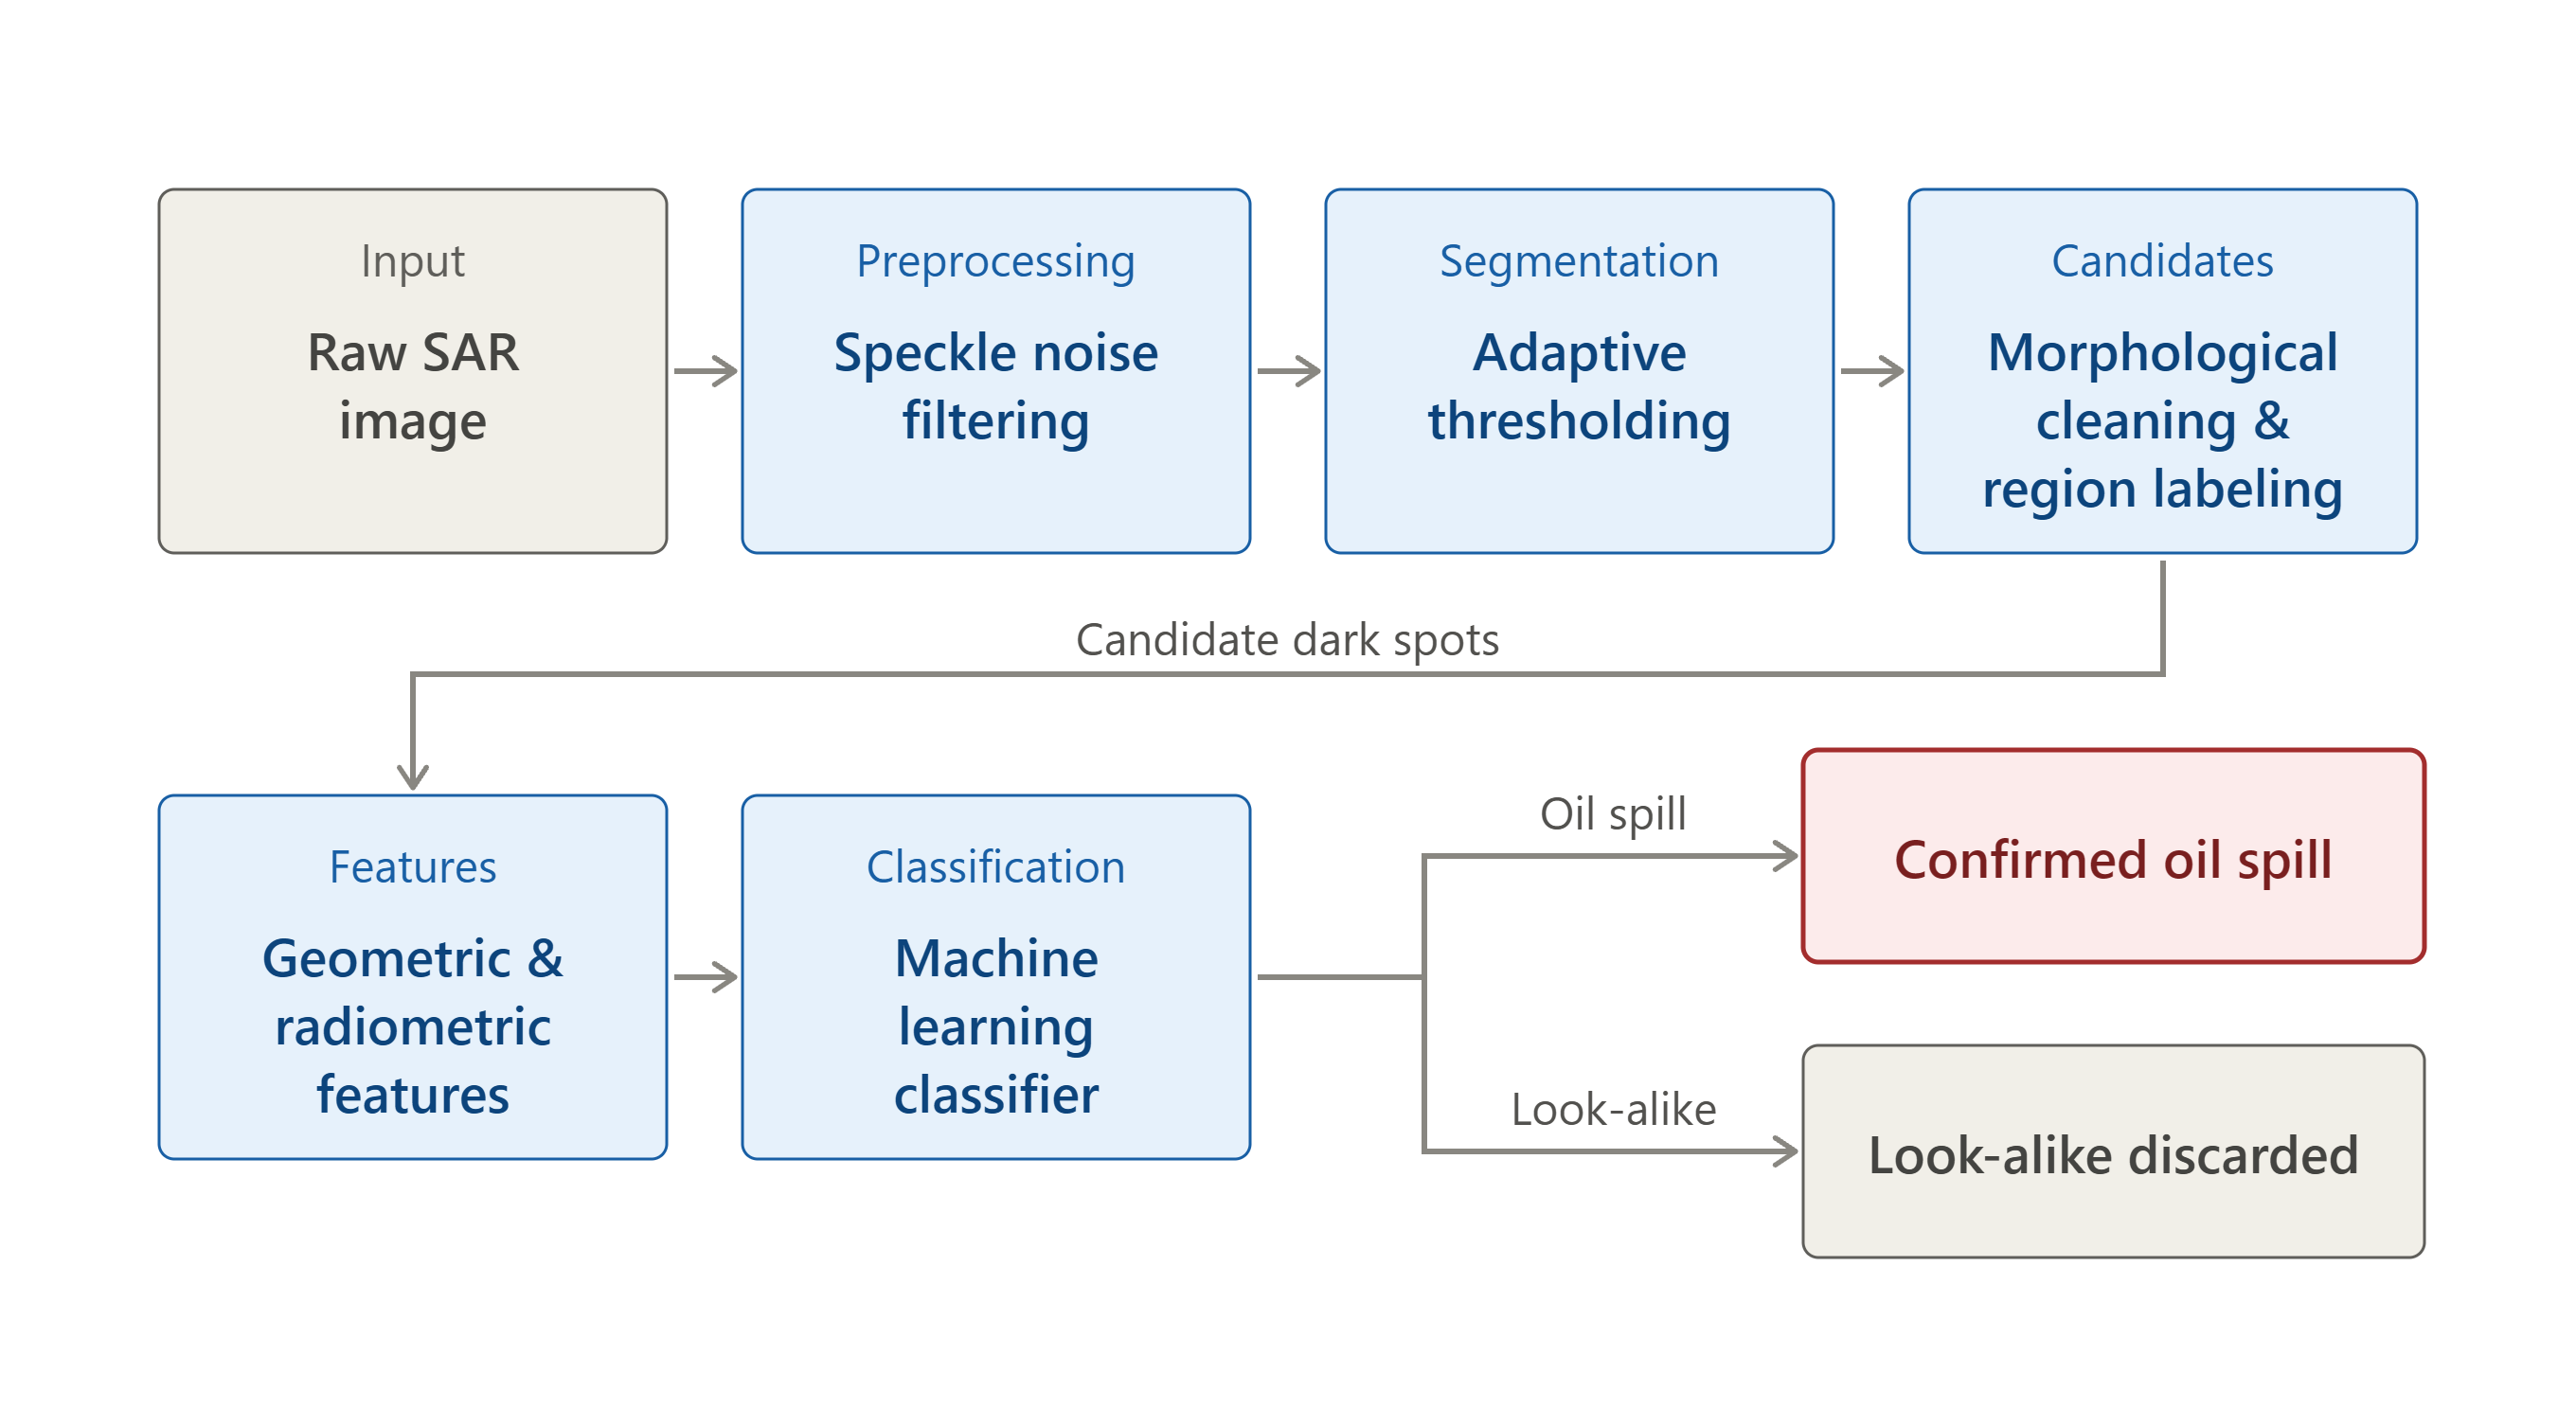
\includegraphics[width=0.88\linewidth, height=0.28\textheight, keepaspectratio]{figures/sar_oil_spill_detection_pipeline.png}
\caption{Kiến trúc 2 giai đoạn (6 khối chức năng) của quy trình phát hiện vết dầu loang từ ảnh SAR.}
\label{fig:pipeline_overview_ch3}
\end{figure}

Luồng biến đổi dữ liệu giữa các khối được quy định cụ thể qua Bảng~\ref{tab:luong_du_lieu_pipeline}:
\begin{enumerate}
    \item \textbf{Giai đoạn 1 (Tạo vùng ứng viên):} Chuyển đổi ảnh thô $I \in [0, 1]$ sang $K$ vùng tối ứng viên rời rạc $\{\Omega_1, \dots, \Omega_K\}$ qua lọc Lee MMSE $\mathcal{O}(HW)$, phân ngưỡng Otsu, lọc diện tích $A_{\min} = 64$ và gán nhãn liên thông 8 hướng.
    \item \textbf{Giai đoạn 2 (Phân loại vùng):} Trích xuất vector 8 đặc trưng $\mathbf{x}_i \in \mathbb{R}^8$ và thẩm định bằng LinearSVM; các vùng có $\mathbf{z}_i^T \mathbf{w} \le 0$ bị loại bỏ, các vùng có $\mathbf{z}_i^T \mathbf{w} > 0$ được giữ lại trong mặt nạ dự đoán $\hat{M}$.
\end{enumerate}

\begin{table}[!htbp]
\centering
\small
\caption{Đầu vào, phép toán và kiểu dữ liệu đầu ra của các bước trong pipeline đã khóa.}
\label{tab:luong_du_lieu_pipeline}
\begin{tabular}{|c|p{2.8cm}|p{4.6cm}|p{4.0cm}|}
\hline
\textbf{Bước} & \textbf{Dữ liệu đầu vào} & \textbf{Thuật toán thực thi} & \textbf{Dữ liệu và kiểu đầu ra} \\ \hline
\textbf{1. Tiền xử lý} & Ảnh PNG 8-bit $[0, 255]$ & Ép kiểu và chia cho $255.0$ & Mảng thực $\texttt{float64} \in [0, 1]$ \\ \hline
\textbf{2. Lọc đốm} & Mảng ảnh mức xám & Lọc Lee MMSE $7 \times 7$ ($L=4$) qua bảng tích lũy SAT & Ảnh làm mượt $I_f \in [0, 1]$ \\ \hline
\textbf{3. Phân đoạn} & Ảnh làm mượt $I_f$ & Phân ngưỡng toàn cục Otsu 256 bin ($t^*$) & Mặt nạ nhị phân thô $\texttt{bool}$ \\ \hline
\textbf{4. Hậu xử lý} & Mặt nạ nhị phân thô & Lọc diện tích $A \ge 64$ và gán nhãn liên thông 8 hướng & Bản đồ nhãn $\texttt{int32}$, $K$ vùng ứng viên $\{\Omega_i\}$ \\ \hline
\textbf{5. Đặc trưng} & Bản đồ nhãn và $I_f$ & Trích xuất 4 hình học và 4 bức xạ/biên theo hộp bao lề 5px & Ma trận đặc trưng $K \times 8$ và danh sách vùng \\ \hline
\textbf{6. Phân loại} & Ma trận đặc trưng & Chuẩn hóa Z-score và suy luận LinearSVM ($C=10$) & Mặt nạ nhị phân cuối $\hat{M}$, overlay và JSON vùng \\ \hline
\end{tabular}
\end{table}

\subsection{Cấu trúc thư mục mã nguồn và hệ thống sổ tay thực nghiệm}

Toàn bộ mã nguồn được tổ chức module hóa trong thư mục \texttt{src/sar\_oil/}:
\begin{itemize}
    \item \texttt{data.py}: Đọc cặp ảnh--mask, kiểm kê mã băm (\texttt{manifest.json}) và phân chia tập Train / Validation / Test.
    \item \texttt{core.py}: Các thuật toán xử lý ảnh tự cài đặt bằng NumPy thuần (SAT, lọc Lee, Otsu, Niblack, hình thái học, CCL 8 hướng, 8 đặc trưng vùng).
    \item \texttt{models.py}: Các bộ phân loại tự cài đặt từ đầu (CART theo tiêu chuẩn Gini và LinearSVM tối ưu bằng NAG).
    \item \texttt{pipeline.py} \& \texttt{evaluation.py}: Luồng suy luận độc lập (không nhận nhãn Ground Truth) và đánh giá ghép cặp một-một Hungarian ở ngưỡng $\IoU \ge 0.5$.
    \item \texttt{reference.py}, \texttt{verification.py} \& \texttt{experiments.py}: Hàm tham chiếu thư viện chuẩn (\texttt{SciPy}, \texttt{scikit-image}, \texttt{scikit-learn}), kiểm thử 118 ca biên và quét lưới $110 \times 729$ cấu hình.
\end{itemize}

Hệ thống cung cấp giao diện dòng lệnh \texttt{scripts/sos.py} cùng 5 sổ tay Jupyter Notebook tương tác (\texttt{01\_data\_and\_ground\_truth.ipynb} đến \texttt{05\_final\_pipeline.ipynb}) để trực quan hóa từng bước và tái lập kết quả thực nghiệm.

\section{Thiết kế giả mã thuật toán lọc đốm và phân đoạn}
\label{sec:thuat_toan_loc_phan_nguong}

\subsection{Thuật toán 3.1: Lọc thống kê Lee MMSE tối ưu hóa qua bảng tổng tích lũy}

Thuật toán~\ref{alg:lee_sat} mô tả quy trình khử nhiễu đốm Lee MMSE với chi phí tuyến tính $\mathcal{O}(HW)$ độc lập với bán kính cửa sổ lọc $r$.

\begin{algorithm}[!htbp]
\small\setstretch{1.05}
\caption{Bộ lọc thống kê Lee MMSE tối ưu hóa qua bảng tổng tích lũy}
\label{alg:lee_sat}
\textbf{Đầu vào:} Ảnh mức xám $I \in [0, 1]^{H \times W}$, bán kính cửa sổ $r \in \mathbb{N}$ (kích thước $k = 2r+1$), số looks $L > 0$, hằng số bảo vệ $\varepsilon = 10^{-12}$. \\
\textbf{Đầu ra:} Ảnh sau khử nhiễu $\hat{R} \in [0, 1]^{H \times W}$.
\begin{algorithmic}[1]
\STATE Khởi tạo mảng đệm đối xứng (reflect padding không lặp pixel mép) kích thước $(H+2r) \times (W+2r)$: $\tilde{I} \leftarrow \text{pad}(I, r, \text{mode}=\text{'reflect'})$
\STATE Tính bảng tích lũy bậc 1 và bậc 2: $S(y, x) \leftarrow \sum_{j \le y, i \le x} \tilde{I}(j, i)$, $S_2(y, x) \leftarrow \sum_{j \le y, i \le x} \tilde{I}^2(j, i)$
\STATE Khởi tạo mảng kết quả $\hat{R}$ kích thước $H \times W$
\FOR{mỗi tọa độ $(y, x)$ từ $0$ đến $H-1, W-1$}
    \STATE Xác định tọa độ cửa sổ trên bảng đệm: $y_1 = y, y_2 = y + 2r + 1, x_1 = x, x_2 = x + 2r + 1$
    \STATE Truy vấn tổng mức xám: $\Sigma \leftarrow S(y_2, x_2) - S(y_1, x_2) - S(y_2, x_1) + S(y_1, x_1)$
    \STATE Truy vấn tổng bình phương: $\Sigma_2 \leftarrow S_2(y_2, x_2) - S_2(y_1, x_2) - S_2(y_2, x_1) + S_2(y_1, x_1)$
    \STATE Trung bình và phương sai cục bộ: $m(y, x) \leftarrow \frac{\Sigma}{(2r+1)^2}$, $v(y, x) \leftarrow \max\left( \frac{\Sigma_2}{(2r+1)^2} - m(y, x)^2, 0 \right)$
    \STATE Phương sai nhiễu và trọng số: $\sigma_{\text{noise}}^2 \leftarrow \frac{m(y, x)^2}{L}$, $W(y, x) \leftarrow \max\left(0, \frac{v(y, x) - \sigma_{\text{noise}}^2}{\max(v(y, x), \varepsilon)}\right)$
    \STATE Cập nhật điểm ảnh sau lọc: $\hat{R}(y, x) \leftarrow m(y, x) + W(y, x) \cdot [I(y, x) - m(y, x)]$
\ENDFOR
\RETURN $\hat{R}$
\end{algorithmic}
\end{algorithm}

\subsection{Thuật toán 3.2: Phân ngưỡng tự động toàn cục Otsu trên biểu đồ mức xám}

Thuật toán~\ref{alg:otsu} trình bày giải thuật tìm ngưỡng phân tách tối đa hóa phương sai giữa hai lớp đối tượng theo Otsu.

\begin{algorithm}[!htbp]
\small\setstretch{1.05}
\caption{Phân ngưỡng tự động toàn cục Otsu 256 bin}
\label{alg:otsu}
\textbf{Đầu vào:} Ảnh sau lọc $I_f \in [0, 1]^{H \times W}$, số bin biểu đồ $B = 256$. \\
\textbf{Đầu ra:} Mặt nạ nhị phân ứng viên $B_{\text{mask}} \in \{0, 1\}^{H \times W}$, ngưỡng tối ưu $t^*$, tỷ số phương sai $\eta$.
\begin{algorithmic}[1]
\STATE Tính biểu đồ tần số $256$ bin trên $[0, 1]$: $H_c \leftarrow \text{histogram}(I_f, \text{bins}=256)$
\STATE Xác suất và tâm bin: $p(i) \leftarrow \frac{H_c(i)}{H \cdot W}$, $c(i) \leftarrow \frac{i + 0.5}{256}$ với $i = 0, \dots, 255$
\STATE Khởi tạo: $\mu_T \leftarrow \sum_{i=0}^{255} c(i) \cdot p(i)$, $\sigma_T^2 \leftarrow \sum_{i=0}^{255} (c(i) - \mu_T)^2 \cdot p(i)$
\IF{$\sigma_T^2 \le 10^{-12}$ (ảnh hằng hoặc gần hằng)}
    \RETURN $B_{\text{mask}} \leftarrow \mathbf{0}_{H \times W}$, $t^* \leftarrow 0.0$, $\eta \leftarrow 0.0$
\ENDIF
\STATE Khởi tạo $\omega_0 \leftarrow 0$, $\mu_{\text{sum}} \leftarrow 0$, $\sigma_{B,\max}^2 \leftarrow -1$, $t^* \leftarrow 0$
\FOR{$t = 0$ đến $254$}
    \STATE $\omega_0 \leftarrow \omega_0 + p(t)$, $\omega_1 \leftarrow 1.0 - \omega_0$
    \IF{$\omega_0 == 0$ hoặc $\omega_1 == 0$}
        \STATE Tiếp tục vòng lặp tiếp theo
    \ENDIF
    \STATE $\mu_{\text{sum}} \leftarrow \mu_{\text{sum}} + c(t) \cdot p(t)$; $\mu_0 \leftarrow \frac{\mu_{\text{sum}}}{\omega_0}$, $\mu_1 \leftarrow \frac{\mu_T - \mu_{\text{sum}}}{\omega_1}$
    \STATE Phương sai giữa hai lớp: $\sigma_B^2 \leftarrow \omega_0 \cdot \omega_1 \cdot (\mu_0 - \mu_1)^2$
    \IF{$\sigma_B^2 > \sigma_{B,\max}^2$}
        \STATE $\sigma_{B,\max}^2 \leftarrow \sigma_B^2$; $t^* \leftarrow c(t)$
    \ENDIF
\ENDFOR
\STATE Sinh mặt nạ ứng viên vùng tối: $B_{\text{mask}}(y, x) \leftarrow [I_f(y, x) < t^*]$; tỷ số phân tách: $\eta \leftarrow \frac{\sigma_{B,\max}^2}{\sigma_T^2}$
\RETURN $B_{\text{mask}}, t^*, \eta$
\end{algorithmic}
\end{algorithm}

\section{Thiết kế giả mã trích xuất đặc trưng và phân loại học máy}
\label{sec:thuat_toan_vung_phan_loai}

\subsection{Thuật toán 3.3: Gán nhãn liên thông 8 hướng và trích xuất 8 đặc trưng vùng}

Thuật toán~\ref{alg:ccl_features} mô tả quy trình chuyển đổi mặt nạ nhị phân thành tập các đối tượng vùng rời rạc và tính toán vector đặc trưng vật lý $\mathbb{R}^8$.

\begin{algorithm}[!htbp]
\small\setstretch{1.05}
\caption{Gán nhãn liên thông 8 hướng và trích xuất đặc trưng vùng theo hộp bao cục bộ}
\label{alg:ccl_features}
\textbf{Đầu vào:} Mặt nạ nhị phân $B_{\text{clean}} \in \{0, 1\}^{H \times W}$, ảnh lọc $I_f \in [0, 1]^{H \times W}$, ngưỡng $A_{\min} = 64$. \\
\textbf{Đầu ra:} Danh sách $K$ vùng ứng viên kèm vector đặc trưng $\{\mathbf{x}_i \in \mathbb{R}^8\}_{i=1}^K$.
\begin{algorithmic}[1]
\STATE Gán nhãn liên thông 8 hướng qua RLE và Union-Find: $L_{\text{map}} \leftarrow \text{connected\_components}(B_{\text{clean}}, \text{connectivity}=8)$
\STATE Thống kê diện tích $A_k \leftarrow |\{(y, x) \mid L_{\text{map}}(y, x) == k\}|$ và lọc $\mathcal{K} \leftarrow \{k \mid A_k \ge A_{\min}\}$; khởi tạo $\mathcal{R} \leftarrow \emptyset$
\FOR{mỗi nhãn vùng $k \in \mathcal{K}$}
    \STATE Tọa độ hộp bao mở rộng lề 5px: $y_0 = \max(0, y_{\min}-5), y_1 = \min(H, y_{\max}+6), x_0 = \max(0, x_{\min}-5), x_1 = \min(W, x_{\max}+6)$
    \STATE Cắt mảng con $M_{\text{sub}} \leftarrow (L_{\text{map}}[y_0:y_1, x_0:x_1] == k)$ và $I_{\text{sub}} \leftarrow I_f[y_0:y_1, x_0:x_1]$
    \STATE $f_0 \leftarrow A_k / (H \cdot W)$; $f_2 \leftarrow A_k / ((y_{\max} - y_{\min} + 1)(x_{\max} - x_{\min} + 1))$
    \STATE Trị riêng hiệp phương sai tọa độ $\lambda_1 \le \lambda_2 \implies f_1 \leftarrow \sqrt{\frac{\lambda_2 + 10^{-6}}{\lambda_1 + 10^{-6}}}$; chu vi cạnh lưới $P_k \implies f_3 \leftarrow \frac{P_k^2}{4\pi A_k}$
    \STATE $f_4 \leftarrow \text{mean}(I_{\text{sub}}[M_{\text{sub}}])$; $f_5 \leftarrow \text{std}(I_{\text{sub}}[M_{\text{sub}}])$
    \STATE Vành biên trong $\partial M \leftarrow M_{\text{sub}} \setminus (M_{\text{sub}} \ominus B_1) \implies f_6 \leftarrow \text{mean}(\|\nabla I_{\text{sub}}\|[\partial M])$
    \STATE Vành đai nền 5px $\text{Ring} \leftarrow (M_{\text{sub}} \oplus B_5) \cap \{L_{\text{sub}} == 0\}$, tính $\mu_{\text{bg}} \implies f_7 \leftarrow \frac{\mu_{\text{bg}} - f_4}{|\mu_{\text{bg}}| + 10^{-6}}$
    \STATE Thêm vector đặc trưng $\mathbf{x}_k = [f_0, f_1, f_2, f_3, f_4, f_5, f_6, f_7]^T$ vào danh sách $\mathcal{R}$
\ENDFOR
\RETURN $\mathcal{R}$
\end{algorithmic}
\end{algorithm}

\subsection{Thuật toán 3.4: Huấn luyện mô hình LinearSVM bằng Nesterov Accelerated Gradient}

Thuật toán~\ref{alg:linearsvm_nag} trình bày chi tiết thuật toán tối ưu hóa lồi có điều chuẩn $L_2$ với hàm mất mát Squared-Hinge Loss.

\begin{algorithm}[!htbp]
\small\setstretch{1.05}
\caption{Huấn luyện LinearSVM bằng gradient tăng tốc Nesterov (NAG)}
\label{alg:linearsvm_nag}
\textbf{Đầu vào:} Ma trận đặc trưng $\mathbf{Z} \in \mathbb{R}^{n \times 9}$ (kèm bias 1), nhãn $y^* \in \{-1, +1\}^n$, $C = 10.0$, $\text{tol} = 10^{-6}$, $\text{max\_iter} = 1000$. \\
\textbf{Đầu ra:} Vector trọng số tối ưu $\mathbf{w}^* \in \mathbb{R}^9$.
\begin{algorithmic}[1]
\STATE Khởi tạo: $\mathbf{w}_0 \leftarrow \mathbf{0}_9$, $\mathbf{v}_0 \leftarrow \mathbf{0}_9$, $\theta_0 \leftarrow 1.0$, $\eta \leftarrow 1.0 / \rho$, giá trị mục tiêu $J_0 \leftarrow J(\mathbf{w}_0)$ theo~\eqref{eq:svm_objective}
\FOR{$t = 0$ đến $\text{max\_iter}-1$}
    \STATE Điểm thăm dò Nesterov: $\mathbf{y}_t \leftarrow \mathbf{w}_t + \beta_t (\mathbf{w}_t - \mathbf{w}_{t-1})$ với $\beta_t = \frac{\theta_{t-1} - 1}{\theta_t}$
    \STATE Tính vector gradient $\nabla J(\mathbf{y}_t)$ theo công thức~\eqref{eq:svm_gradient}
    \IF{$\|\nabla J(\mathbf{y}_t)\|_\infty \le \text{tol}$}
        \STATE $\mathbf{w}^* \leftarrow \mathbf{y}_t$; Dừng vòng lặp thành công
    \ENDIF
    \WHILE{$J(\mathbf{y}_t - \eta \nabla J(\mathbf{y}_t)) > J(\mathbf{y}_t) - \frac{\eta}{2}\|\nabla J(\mathbf{y}_t)\|_2^2$}
        \STATE $\eta \leftarrow 0.5 \times \eta$ \COMMENT{Tìm bước nhảy quay lui (backtracking line search)}
    \ENDWHILE
    \STATE Cập nhật điểm mới: $\mathbf{w}_{t+1} \leftarrow \mathbf{y}_t - \eta \nabla J(\mathbf{y}_t)$
    \IF{$(\mathbf{w}_{t+1} - \mathbf{w}_t)^T \nabla J(\mathbf{y}_t) > 0$ (xung lượng đối nghịch)}
        \STATE Kích hoạt thích nghi (adaptive restart): $\mathbf{y}_t \leftarrow \mathbf{w}_t$, $\theta_{t+1} \leftarrow 1.0$
    \ELSE
        \STATE Cập nhật hệ số xung lượng: $\theta_{t+1} \leftarrow \frac{1 + \sqrt{1 + 4\theta_t^2}}{2}$
    \ENDIF
\ENDFOR
\RETURN $\mathbf{w}^*$
\end{algorithmic}
\end{algorithm}

\section{Phân tích độ phức tạp thuật toán và kỹ thuật tối ưu hóa NumPy}
\label{sec:do_phuc_tap_ky_thuat}

\subsection{Phân tích độ phức tạp thời gian và không gian bộ nhớ}

Bảng~\ref{tab:do_phuc_tap} tổng hợp phân tích lý thuyết về độ phức tạp thời gian tính toán và bộ nhớ phụ trợ của các khối chức năng chính trong quy trình phát hiện vết dầu loang, với $H, W$ là kích thước ảnh viễn thám ($256 \times 256$), $B = 256$ là số bin histogram, $K$ là số lượng vùng ứng viên liên thông sau phân đoạn, $n = 20\,000$ là số lượng mẫu huấn luyện mô hình, và $d = 8$ là số chiều vector đặc trưng vùng.

\begin{table}[!htbp]
\centering
\small
\caption{Phân tích độ phức tạp thời gian và không gian bộ nhớ của từng bước trong pipeline.}
\label{tab:do_phuc_tap}
\begin{tabular}{|l|c|c|p{5.5cm}|}
\hline
\textbf{Khối chức năng} & \textbf{Thời gian} & \textbf{Bộ nhớ} & \textbf{Ghi chú kỹ thuật} \\ \hline
\textbf{1. Bảng tích lũy SAT} & $\mathcal{O}(HW)$ & $\mathcal{O}(HW)$ & Tính 2 bảng $S$ và $S_2$ với đúng một lượt duyệt mảng 2 chiều bằng \texttt{np.cumsum}. \\ \hline
\textbf{2. Lọc Lee MMSE} & $\mathcal{O}(HW)$ & $\mathcal{O}(HW)$ & Truy vấn 4 góc SAT trong $\mathcal{O}(1)$, hoàn toàn độc lập với kích thước cửa sổ $k \times k$. \\ \hline
\textbf{3. Phân ngưỡng Otsu} & $\mathcal{O}(HW + B)$ & $\mathcal{O}(B)$ & Quét ảnh tạo histogram $\mathcal{O}(HW)$, quét tìm $t^*$ tối ưu trên $B=256$ bin trong $\mathcal{O}(B)$. \\ \hline
\textbf{4. Gán nhãn liên thông CCL} & $\mathcal{O}(HW \cdot \alpha)$ & $\mathcal{O}(HW)$ & Kỹ thuật RLE kết hợp Union-Find nén đường đi, $\alpha(\cdot) \le 4$ là hàm nghịch đảo Ackermann. \\ \hline
\textbf{5. Trích xuất đặc trưng} & $\mathcal{O}(K \cdot \bar{A})$ & $\mathcal{O}(\bar{A})$ & Duyệt theo hộp bao cục bộ mở rộng lề 5px, $\bar{A}$ là diện tích trung bình của hộp bao vùng. \\ \hline
\textbf{6. Suy luận LinearSVM} & $\mathcal{O}(K \cdot d)$ & $\mathcal{O}(K)$ & Tích vô hướng vector nhanh qua phép nhân ma trận mảng $\mathbf{Z} \mathbf{w}$. \\ \hline
\textbf{7. Huấn luyện NAG SVM} & $\mathcal{O}(T \cdot n \cdot d)$ & $\mathcal{O}(n \cdot d)$ & $T = 177$ vòng lặp hội tụ, vector hóa toàn bộ phép tính sai số lề trên mảng $20\,000 \times 9$. \\ \hline
\end{tabular}
\end{table}

\subsection{Các khó khăn kỹ thuật và giải pháp tối ưu hóa trên NumPy}

Trong quá trình cài đặt hệ thống bằng NumPy thuần, 4 thách thức kỹ thuật cốt lõi được giải quyết:
\begin{enumerate}
    \item \textbf{Hiện tượng tràn số nguyên \texttt{uint8} và triệt tiêu số học:}
    Tính trực tiếp tổng bình phương trên \texttt{uint8} sẽ tràn qua $255$, trong khi công thức $\E[I^2] - (\E[I])^2$ trên số thực có thể nhận giá trị âm siêu nhỏ ($\sim -10^{-17}$) tại vùng ảnh hằng do sai số dấu phẩy động. Giải pháp: ép kiểu mảng ảnh sang $\texttt{float64} \in [0, 1]$ ngay từ đầu và áp dụng phép kẹp dưới phương sai cục bộ $v(x, y) = \max\left( \frac{\Sigma_2}{(2r+1)^2} - m(x, y)^2, 0 \right)$.
    \item \textbf{Chuẩn hóa cơ chế đệm biên đối xứng (reflect padding):}
    Đệm biên bằng $0$ (zero-padding) tạo dải tối nhân tạo ở 4 cạnh khiến Otsu nhận nhầm viền ảnh là dầu, còn đệm lặp điểm ảnh mép (replicate) làm lệch phương sai biên. Giải pháp: áp dụng đệm phản xạ không lặp điểm ảnh mép ($I[-1] = I[1]$), khớp với \texttt{mode='mirror'} của \texttt{scipy.ndimage.generic\_filter}.
    \item \textbf{Xử lý các ca biên suy biến (degenerate edge cases):}
    Để tránh lỗi $\texttt{NaN} / \texttt{Inf}$: (i) với ảnh hằng ($\sigma_T^2 \le 10^{-12}$), Otsu trả về mặt nạ toàn $0$ và $\eta = 0.0$; (ii) với vùng suy biến thẳng hàng ($\lambda_1 = 0$), độ thuôn dài cộng hằng số $\varepsilon = 10^{-6}$ vào cả tử và mẫu $\sqrt{(\lambda_2 + \varepsilon)/(\lambda_1 + \varepsilon)}$; (iii) với khung ảnh ngập dầu làm rỗng vành đai 5px, $\mu_{\text{bg}}$ tự động chuyển sang tính trên phần nền còn lại hoặc trung bình toàn ảnh.
    \item \textbf{Tăng tốc tính toán bằng kỹ thuật vector hóa và hộp bao cục bộ:}
    Thay vì duyệt toàn bộ khung ảnh $256 \times 256$ cho từng vùng liên thông (mất $>1.5\text{ s}$ cho ảnh 50 ứng viên), phạm vi tính gradient Sobel và phép giãn vành đai được cắt gọn vào hộp bao cục bộ mở rộng lề 5px ($[y_{\min}-5 : y_{\max}+6, x_{\min}-5 : x_{\max}+6]$), giảm thời gian trích xuất xuống dưới $8\text{ ms/ảnh}$.
\end{enumerate}

\section{Kiểm chứng tính đúng đắn số học so với thư viện chuẩn}
\label{sec:kiem_chung_thu_vien}

\subsection{Đối chứng số học các thuật toán xử lý ảnh trên tập ảnh viễn thám thực tế}

Để kiểm chứng tính đúng đắn của các thuật toán tự cài đặt bằng NumPy thuần, giao thức kiểm thử đối chứng kép được thiết lập:
\begin{enumerate}
    \item Bộ kiểm thử đơn vị tự động gồm 118 phép kiểm định ca biên tổng hợp (\texttt{tests/test\_core.py} và \texttt{src/sar\_oil/verification.py}), bao gồm ảnh toàn số 0, ảnh toàn số 1, ảnh nhiễu ngẫu nhiên, ảnh có kích thước lẻ/chẵn, và các đối tượng chạm sát biên khung hình. Toàn bộ 118 ca kiểm thử đều đạt kết quả $\texttt{passed} = \texttt{True}$.
    \item Kiểm chứng thực nghiệm trên 8 ảnh SAR thực tế được lấy mẫu đại diện từ tập Validation với hạt giống $\texttt{seed} = 2026$. Trên 8 ảnh này, hệ thống thực thi song song toàn bộ 24 cấu hình thuật toán khác nhau giữa bản tự cài NumPy và bản thư viện chuẩn (\texttt{SciPy}, \texttt{scikit-image}), tạo thành tổng cộng 192 phép đối chứng số học.
\end{enumerate}

Bảng~\ref{tab:doi_chung_sai_so_thu_vien} tổng hợp sai số tuyệt đối lớn nhất ($\max |\Delta|$) và sai số bình phương trung bình lớn nhất ($\text{MSE}$) ghi nhận trên toàn bộ 8 ảnh viễn thám thực tế.

\begin{table}[!htbp]
\centering
\small
\caption{Kết quả đối chứng số học giữa triển khai NumPy thuần và hàm thư viện chuẩn (\texttt{SciPy}, \texttt{scikit-image}) trên 8 ảnh Validation thực tế (24 cấu hình $\times 8$ ảnh $= 192$ phép kiểm định).}
\label{tab:doi_chung_sai_so_thu_vien}
\resizebox{\textwidth}{!}{%
\begin{tabular}{|l|l|c|c|}
\hline
\textbf{Nhóm thuật toán} & \textbf{Cấu hình kiểm thử} & \textbf{Sai số tuyệt đối lớn nhất} & \textbf{MSE lớn nhất} \\ \hline
\textbf{Lọc không gian} & Không lọc (\texttt{none}) \& Trung vị $3\times 3, 5\times 5$ & $0.000 \times 10^{0}$ & $0.000 \times 10^{0}$ \\ \cline{2-4}
& Lọc Gaussian $\sigma \in \{0.8, 1.2\}$ & $3.331 \times 10^{-16}$ & $6.102 \times 10^{-33}$ \\ \cline{2-4}
& Lọc Lee $3 \times 3$ \& $5 \times 5$ ($L \in \{1, 4\}$) & $\le 1.382 \times 10^{-11}$ & $\le 5.785 \times 10^{-26}$ \\ \cline{2-4}
& Lọc Lee $7 \times 7$ ($L=1$) & $6.274 \times 10^{-13}$ & $2.584 \times 10^{-27}$ \\ \cline{2-4}
& \textbf{Lọc Lee $7 \times 7$ ($L=4$) [Chọn]} & $\mathbf{2.737 \times 10^{-12}}$ & $\mathbf{4.337 \times 10^{-27}}$ \\ \hline
\textbf{Phân ngưỡng} & Ngưỡng toàn cục Otsu (256 bin) & $0.000 \times 10^{0}$ & $0.000 \times 10^{0}$ \\ \cline{2-4}
& Niblack $15\times 15, 31\times 31, 51\times 51$ ($k \in \{0.2, 0.5, 0.8\}$) & $0.000 \times 10^{0}$ & $0.000 \times 10^{0}$ \\ \hline
\textbf{Hình thái \&} & Không hình thái (\texttt{none}) \& Đóng (\texttt{close}) & $\le 3.109 \times 10^{-14}$ & $\le 2.338 \times 10^{-30}$ \\ \cline{2-4}
\textbf{Đặc trưng vùng} & Mở -- Đóng (\texttt{open\_close}) & $1.101 \times 10^{-13}$ & $1.367 \times 10^{-29}$ \\ \hline
\end{tabular}%
}
\end{table}

Số liệu trong Bảng~\ref{tab:doi_chung_sai_so_thu_vien} cho thấy: (i) Otsu, Niblack và lọc trung vị đạt sai số tuyệt đối $0.000$ (trùng khớp từng điểm ảnh với \texttt{scikit-image}); (ii) lọc Gaussian lệch ở mức $10^{-16}$ (giới hạn machine epsilon 64-bit); và (iii) lọc Lee MMSE lệch tối đa $1.382 \times 10^{-11}$ do khác biệt thứ tự cộng dồn dấu phẩy động giữa bảng tích lũy SAT và cửa sổ trượt \texttt{SciPy}.

\subsection{Đối chứng bộ phân loại học máy tự cài đặt với scikit-learn}

Mô hình LinearSVM và CART tự cài đặt trong \texttt{models.py} được đối sánh trực tiếp với \texttt{LinearSVC} và \texttt{DecisionTreeClassifier} của \texttt{scikit-learn} trên cùng tập đặc trưng Validation ($9\,287$ mẫu ứng viên).

\begin{table}[!htbp]
\centering
\small
\caption{Đối chứng hiệu năng, độ đồng thuận dự đoán và giá trị mục tiêu giữa mô hình tự cài đặt bằng NumPy và thư viện \texttt{scikit-learn}.}
\label{tab:doi_chung_classifier}
\resizebox{\textwidth}{!}{%
\begin{tabular}{|l|c|c|c|c|c|}
\hline
\textbf{Mô hình} & \textbf{Độ đồng thuận} & \textbf{F1 NumPy} & \textbf{F1 sklearn} & \textbf{Giá trị hàm mục tiêu $J^*$} & \textbf{Hội tụ} \\ \hline
\textbf{CART} & $\mathbf{1.0000}$ ($100\%$) & 0.3373 & 0.3373 & -- & Đạt \\ \hline
\textbf{LinearSVM} & $\mathbf{1.0000}$ ($100\%$) & 0.3403 & 0.3403 & $|J_{\text{NumPy}}^* - J_{\text{sklearn}}^*| = 2.88 \times 10^{-12}$ & Đạt ($177$ vòng) \\ \hline
\end{tabular}%
}
\end{table}

Bảng~\ref{tab:doi_chung_classifier} xác nhận cả hai mô hình tự cài đặt đạt độ đồng thuận dự đoán $\mathbf{100\%}$ ($\text{Agreement} = 1.0000$) trên toàn bộ $9\,287$ mẫu. Bộ giải NAG đạt giá trị mục tiêu $J_{\text{NumPy}}^* = 4.0531228859$, lệch chỉ $2.88 \times 10^{-12}$ so với \texttt{LIBLINEAR} ($J_{\text{sklearn}}^* = 4.0531228859$), và dừng hội tụ sau 177 vòng lặp với $\|\nabla J\|_\infty = 9.94 \times 10^{-7} \le 10^{-6}$.


% CHƯƠNG 4: THỰC NGHIỆM VÀ ĐÁNH GIÁ
\chapter{Thực nghiệm và đánh giá}
\label{chap:thuc_nghiem_danh_gia}
\section{Môi trường thực nghiệm, bộ dữ liệu và các chỉ số đánh giá}
\label{sec:moi_truong_du_lieu_chi_so}

\subsection{Cấu hình môi trường thực nghiệm và liêm chính tái lập}

Toàn bộ thực nghiệm được thực thi trên cấu hình đồng nhất: vi xử lý đa nhân x86\_64 (AVX2), RAM $16.0\text{ GiB}$, hệ điều hành Windows 11 64-bit, Python \texttt{3.13.12} (\texttt{numpy 2.5.4}, \texttt{scipy 1.18.1}, \texttt{scikit-image 0.26.0}, \texttt{scikit-learn 1.9.1}, \texttt{matplotlib 3.11.2}, \texttt{Pillow 13.0.0}). Các thư viện đại số tuyến tính được khóa đơn luồng (\texttt{OMP/MKL/OPENBLAS\_NUM\_THREADS=1}), cố định hạt giống $\texttt{seed} = 2026$ và kiểm chứng toàn vẹn qua mã băm \texttt{manifest\_sha256} trong \texttt{results/sos/run\_manifest.json}.

\subsection{Bộ dữ liệu chuẩn Refined Deep-SAR Oil Spill (SOS)}

Nghiên cứu sử dụng bộ dữ liệu công khai \textit{Refined Deep-SAR Oil Spill (SOS)}~\cite{zuenko2025refined}, kế thừa từ công trình của Zhu và cộng sự~\cite{zhu2022oil}, gồm 21 cảnh SAR độ phân giải cao từ hai sự cố tràn dầu lớn được cắt thành các mảnh $256 \times 256$ điểm ảnh (Bảng~\ref{tab:thong_ke_sos}):
\begin{enumerate}
    \item \textbf{Mỏ dầu Al-Khafji (Vịnh Ba Tư, 2017):} 7 cảnh vệ tinh Sentinel-1A (băng C, $\sim 5.6\text{ cm}$, phân cực VV, chế độ IW mức GRD, độ phân giải $5\text{ m} \times 20\text{ m}$).
    \item \textbf{Giàn khoan Deepwater Horizon (Vịnh Mexico, 2010):} 14 cảnh vệ tinh ALOS PALSAR (băng L, $\sim 23.6\text{ cm}$, phân cực HH, mức 1.5, độ phân giải $12.5\text{ m}$).
\end{enumerate}

\begin{table}[!htbp]
\centering
\small
\caption{Thống kê phân chia các tập dữ liệu trong nghiên cứu.}
\label{tab:thong_ke_sos}
\resizebox{\textwidth}{!}{%
\begin{tabular}{|l|c|c|p{6.0cm}|}
\hline
\textbf{Phân tập dữ liệu} & \textbf{Cảm biến vệ tinh} & \textbf{Số lượng ảnh} & \textbf{Vai trò và mục đích sử dụng} \\ \hline
\textbf{Train (Huấn luyện)} & Sentinel-1A & $2\,683$ ảnh & Trích xuất mẫu huấn luyện LinearSVM và CART, tính thống kê Z-score. \\ \hline
\textbf{Validation (Kiểm định)} & Sentinel-1A & $671$ ảnh & Độc quyền phục vụ sàng lọc 110 cấu hình lọc/ngưỡng và 729 cấu hình mô hình vùng. \\ \hline
\textbf{Test (Kiểm thử độc lập)} & Sentinel-1A & $839$ ảnh & Đánh giá khách quan cấu hình chiến thắng sau khi toàn bộ quy trình đã đóng băng. \\ \hline
\textbf{External Test (Ngoài cảm biến)} & ALOS PALSAR & $776$ ảnh & Kiểm tra khả năng chuyển giao ngoài miền cảm biến với mô hình đóng băng từ Sentinel-1A. \\ \hline
\textbf{Tổng cộng sử dụng} & \multicolumn{3}{c|}{\textbf{4\,969 ảnh viễn thám $256 \times 256$}} \\ \hline
\end{tabular}%
}
\end{table}

\subsection{Giao thức phân tầng theo 5 chế độ diện tích dầu}

Dựa trên tỷ lệ diện tích dầu $r = \frac{1}{HW}\sum_{x,y} G(x, y)$ trên mặt nạ Ground Truth, các ảnh được phân tầng thành 5 chế độ ($R_0 \to R_4$): \textbf{$R_0$ (Biển sạch, $r = 0$)} kiểm định tỷ lệ báo nhầm; \textbf{$R_1$ (Vết dầu nhỏ, $0 < r < 0.05$)}; \textbf{$R_2$ (Dải dầu trung bình, $0.05 \le r < 0.50$)}; \textbf{$R_3$ (Dầu diện rộng, $0.50 \le r < 0.95$)}; và \textbf{$R_4$ (Ngập dầu toàn phần, $r \ge 0.95$)}. Hình~\ref{fig:sos_dataset_regimes} cho thấy histogram hai đỉnh phân tách rõ chỉ xuất hiện ở $R_2$, trong khi ở $R_0$ và $R_4$, histogram đơn đỉnh khiến ngưỡng Otsu thô bị ép chia đôi ảnh và sinh ra các đốm báo nhầm.

\begin{figure}[!htbp]
\centering
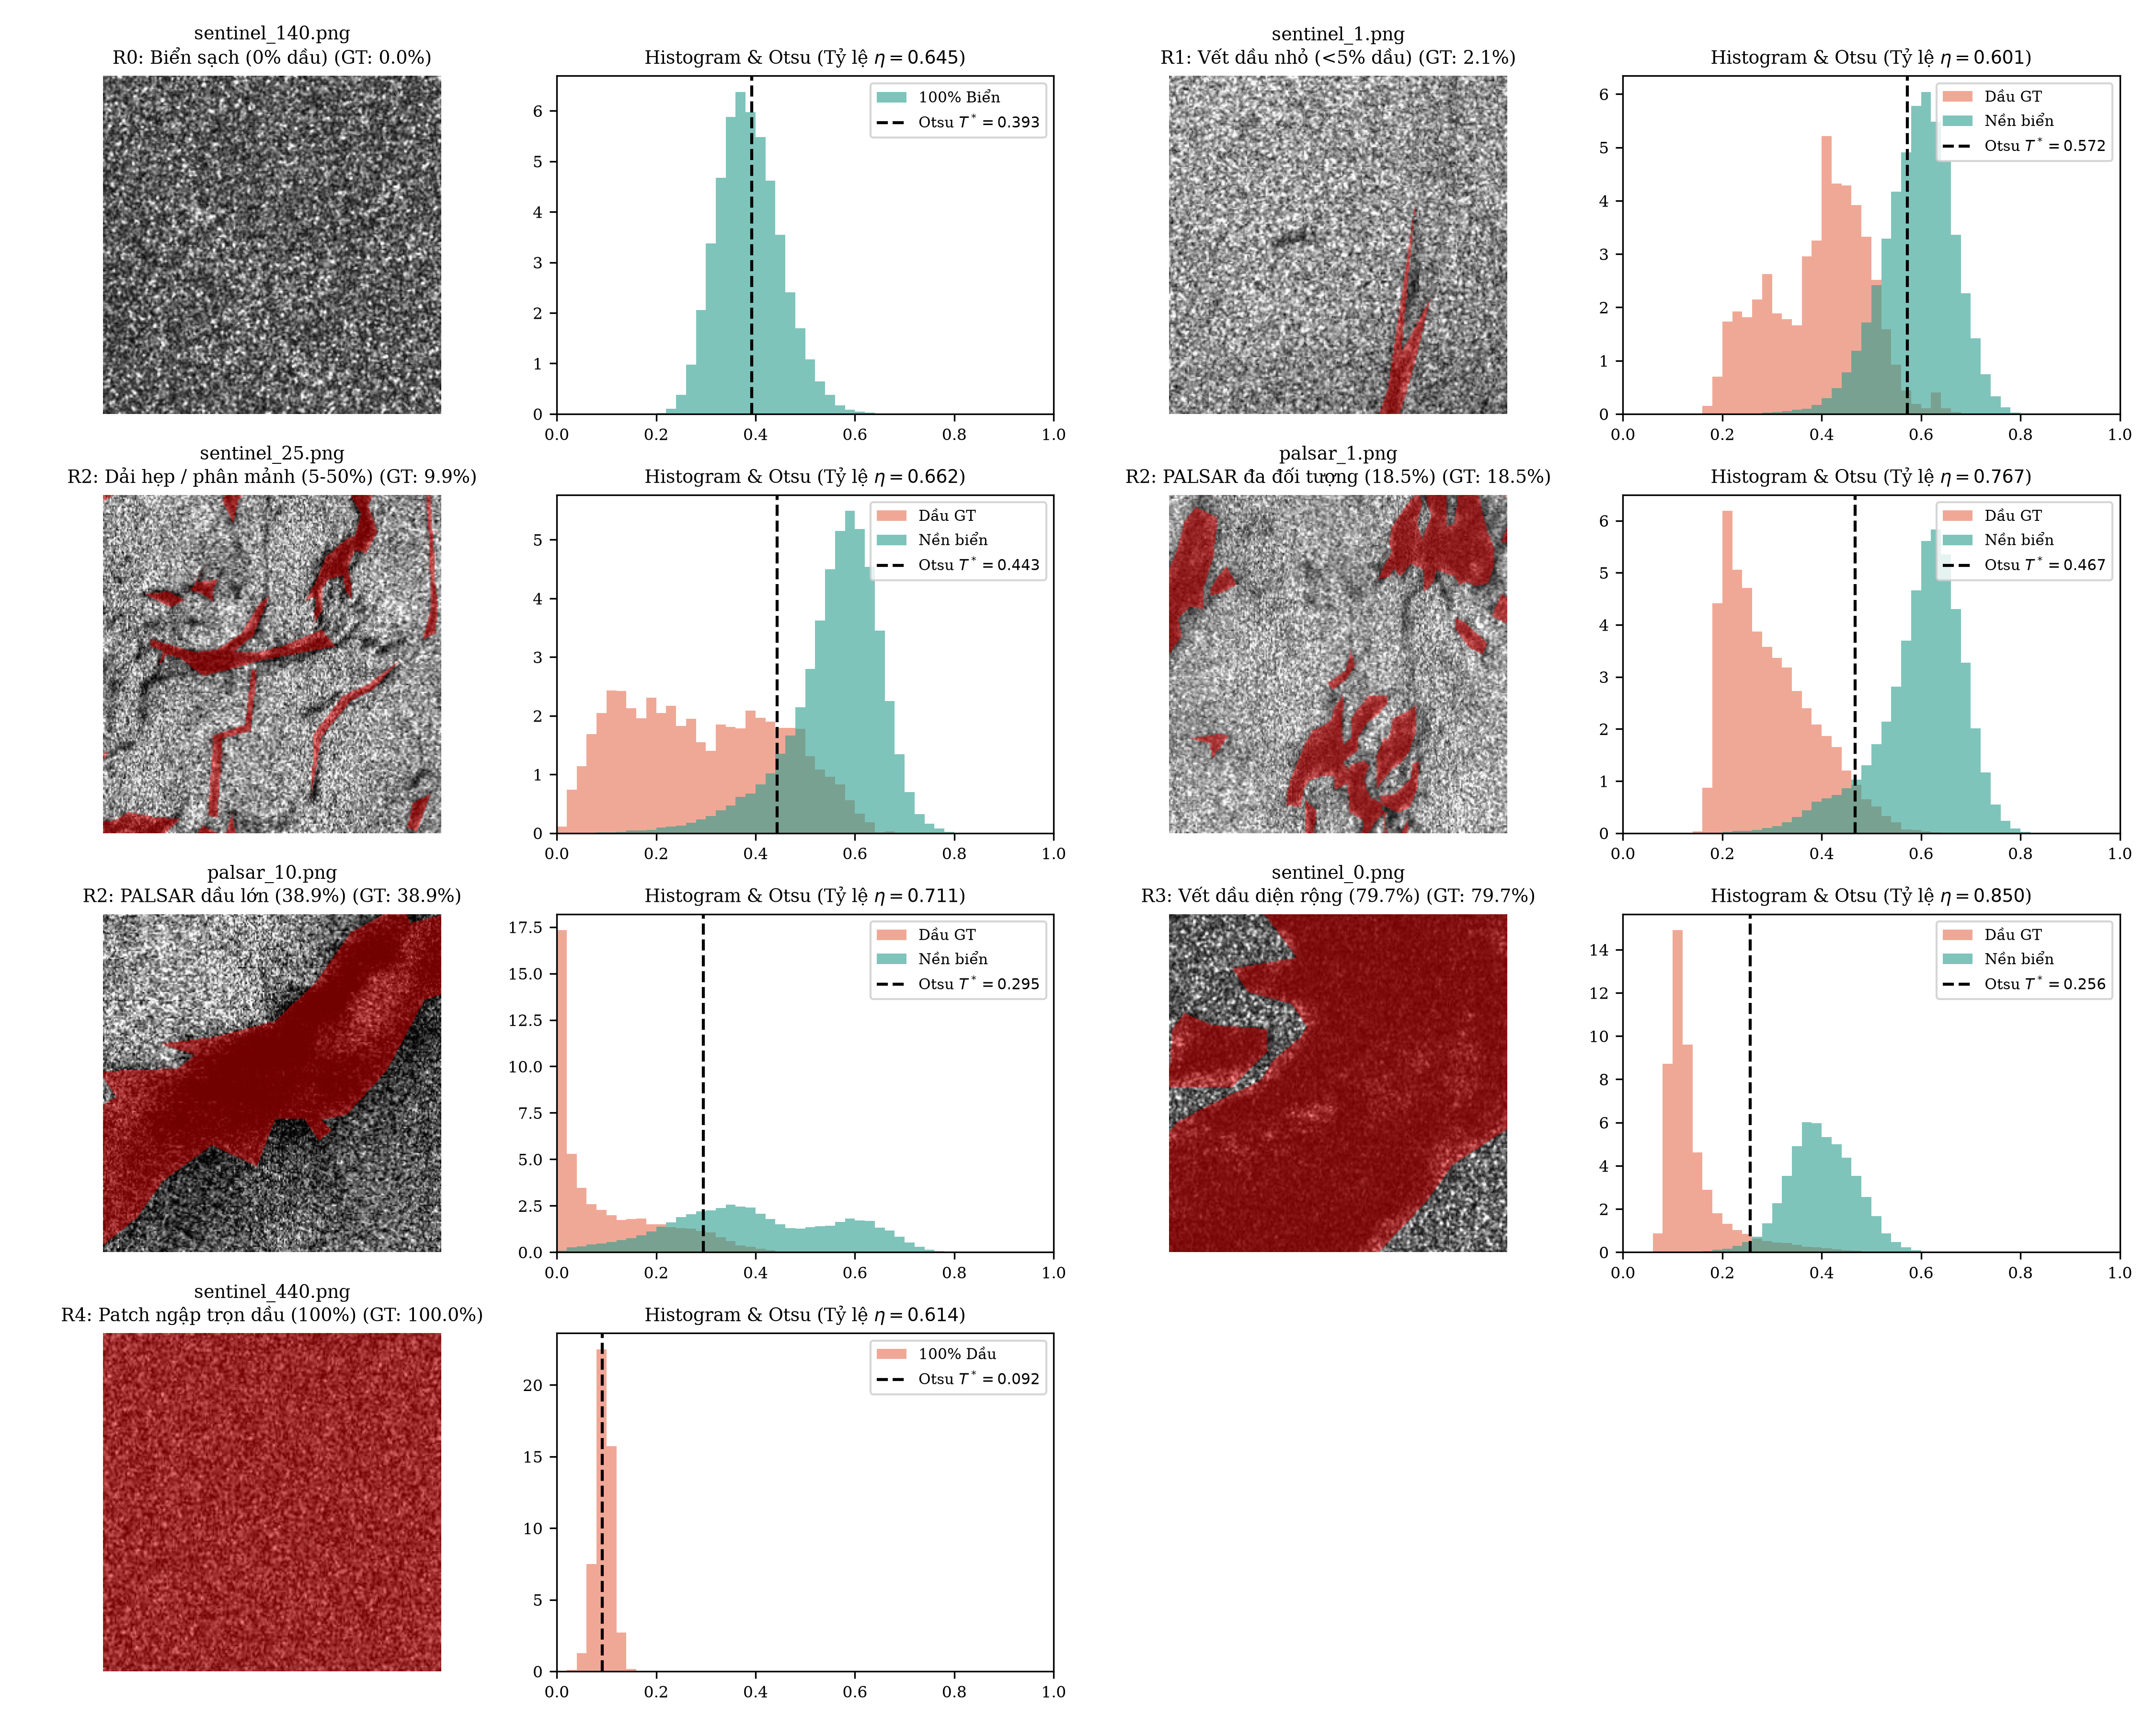
\includegraphics[width=0.90\textwidth]{figures/fig2_sos_dataset_regimes.png}
\caption{Mẫu ảnh SAR thực tế, mặt nạ Ground Truth và phân bố biểu đồ mức xám histogram qua 5 chế độ diện tích dầu ($R_0 \to R_4$).}
\label{fig:sos_dataset_regimes}
\end{figure}

\subsection{Hệ thống các chỉ số đánh giá định lượng}

Nghiên cứu áp dụng đồng thời hai cấp độ đánh giá độc lập:
\begin{enumerate}
    \item \textbf{Đánh giá cấp đối tượng theo thuật toán Hungarian ($\IoU \ge 0.5$):}
    Mặt nạ dự đoán $\hat{M}$ và Ground Truth $G$ được phân rã thành các đối tượng liên thông $\{\hat{\Omega}_p\}_{p=1}^P$ và $\{G_q\}_{q=1}^Q$. Ma trận $\IoU_{p, q} = |\hat{\Omega}_p \cap G_q| / |\hat{\Omega}_p \cup G_q|$ được giải ghép cặp một-một bằng thuật toán Hungarian; cặp đạt $\IoU_{p, q} \ge 0.5$ được tính là True Positive (TP), vùng dự đoán dư là False Positive (FP), và đối tượng bỏ sót là False Negative (FN). Các chỉ số vi mô (Micro-averaging) trên toàn tập ảnh gồm:
    \begin{equation}
    \text{Precision} = \frac{\sum \text{TP}}{\sum \text{TP} + \sum \text{FP}}, \quad \text{Recall} = \frac{\sum \text{TP}}{\sum \text{TP} + \sum \text{FN}}, \quad \text{Object F1} = \frac{2 \sum \text{TP}}{2 \sum \text{TP} + \sum \text{FP} + \sum \text{FN}}
    \end{equation}
    Ngoài ra, nghiên cứu báo cáo trung bình vĩ mô từng ảnh ($\text{mean} \pm \text{SD}$), tỷ lệ thu hồi vùng chạm biên (\textbf{Edge Recall}) và vùng nội bộ (\textbf{Interior Recall}).
    \item \textbf{Đánh giá cấp điểm ảnh (Pixel-level) và mật độ cảnh báo sai:}
    Độ bao phủ diện tích toàn cục và số vùng báo nhầm trung bình mỗi ảnh (\textbf{FP/ảnh}) được tính bởi:
    \begin{equation}
    \text{Pixel IoU} = \frac{\sum |\hat{M} \cap G|}{\sum |\hat{M} \cup G|}, \quad \text{Dice} = \frac{2 \sum |\hat{M} \cap G|}{\sum |\hat{M}| + \sum |G|}
    \end{equation}
\end{enumerate}

\section{Khảo sát có kiểm soát các bộ lọc và phân ngưỡng tạo ứng viên}
\label{sec:thuc_nghiem_loc_nguong}

\subsection{Thiết kế thí nghiệm sàng lọc 110 cấu hình trên tập Validation}

Chất lượng của tập vùng ứng viên ban đầu quyết định trần độ thu hồi của toàn hệ thống: nếu bộ lọc không đủ mạnh, nhiễu đốm sẽ sinh ra hàng vạn mảnh vụn nhỏ; ngược lại, nếu làm mượt quá mức, các dải dầu hẹp sẽ bị xóa nhòa. Để lựa chọn cấu hình tối ưu, nghiên cứu thực hiện khảo sát tích Descartes gồm \textbf{11 bộ lọc không gian} (\texttt{none}; \texttt{median} kích thước $\{3, 5\}$; \texttt{gaussian} $\sigma \in \{0.8, 1.2\}$; \texttt{lee} kích thước $\{3, 5, 7\} \times L \in \{1, 4\}$) và \textbf{10 bộ phân ngưỡng} (\texttt{otsu} toàn cục; \texttt{niblack} cục bộ với cửa sổ $\{15, 31, 51\} \times k \in \{0.2, 0.5, 0.8\}$), tạo thành $110$ tổ hợp chạy trên toàn bộ $671$ ảnh Validation (cố định $A_{\min} = 16$).

\begin{figure}[!htbp]
\centering
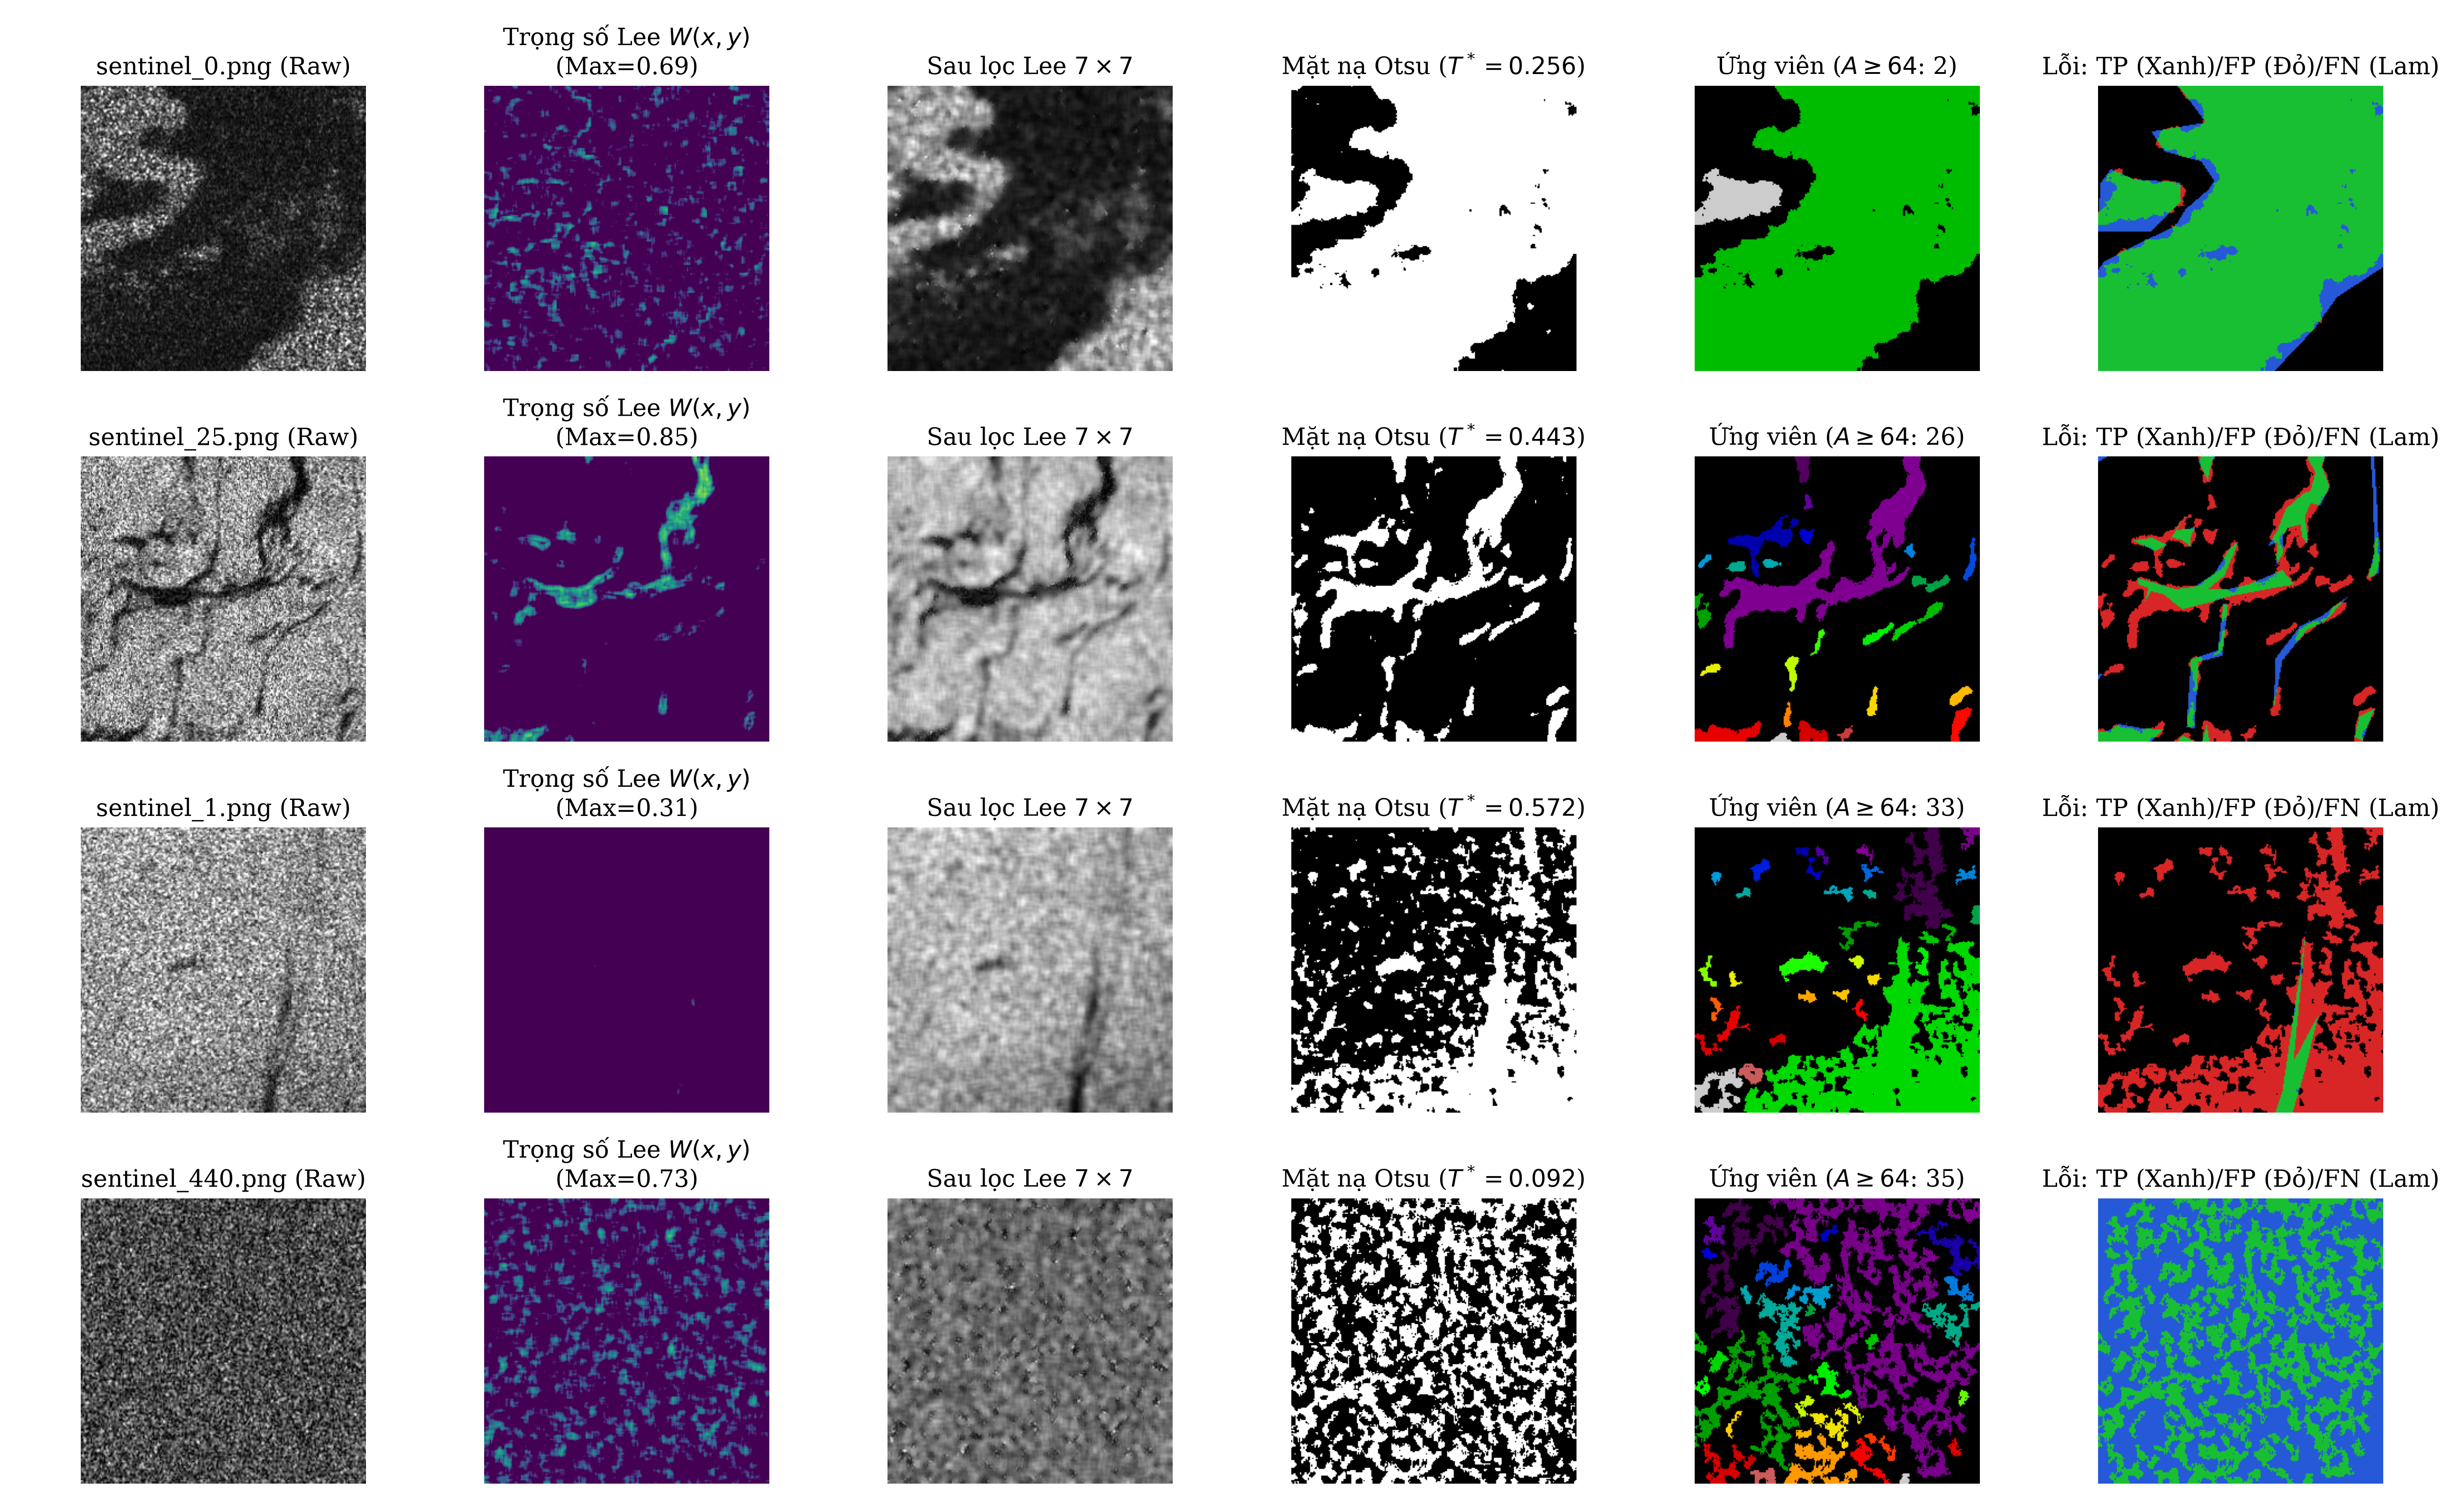
\includegraphics[width=\textwidth]{figures/fig3_step_by_step_pipeline.png}
\caption{Trực quan hóa các bước biến đổi trung gian của quy trình trên 4 cảnh SAR đại diện: Ảnh gốc $\to$ Bản đồ trọng số Lee $W(x, y)$ $\to$ Ảnh sau lọc Lee $7 \times 7$ $\to$ Mặt nạ nhị phân Otsu $\to$ Vùng ứng viên sau lọc diện tích $\ge 64$ $\to$ Bản đồ phân loại lỗi điểm ảnh (Xanh lá: TP, Đỏ: FP, Lam: FN).}
\label{fig:step_by_step_pipeline}
\end{figure}

Hình~\ref{fig:step_by_step_pipeline} trực quan hóa các bước trung gian của quy trình. Bảng~\ref{tab:filter_benchmark} tổng hợp kết quả định lượng chi tiết của 13 cấu hình lọc không gian tiêu biểu kết hợp với phân ngưỡng Otsu, kèm khoảng tin cậy Bootstrap 95\% của mức chênh lệch $\Delta\text{F1}$ tính qua $2\,000$ lần lấy mẫu lại có hoàn lại.

\begin{table}[!htbp]
\centering
\small
\caption{So sánh có kiểm soát 13 cấu hình lọc không gian (cố định phân ngưỡng Otsu, $A_{\min} = 16$) trên 671 ảnh Validation. Khoảng tin cậy Bootstrap 95\% của $\Delta\text{F1}$ so với Lee $7 \times 7$ ($L=4$).}
\label{tab:filter_benchmark}
\resizebox{\textwidth}{!}{%
\begin{tabular}{|l|c|c|c|c|c|c|c|c|}
\hline
\textbf{Cấu hình bộ lọc} & \textbf{TP} & \textbf{FP} & \textbf{FN} & \textbf{Prec} & \textbf{Rec} & \textbf{Cand F1} & \textbf{Pix IoU} & \textbf{$\Delta\text{F1}$ vs. Lee $7\times 7, L=4$ (95\% CI)} \\ \hline
\textit{None (Không lọc)} & 518 & $39\,283$ & $2\,222$ & 0.0130 & 0.1891 & 0.0244 & 0.4272 & $+0.0612 \quad [+0.0534, +0.0693]$ \\ \hline
\textit{Median $3 \times 3$} & 758 & $50\,479$ & $1\,982$ & 0.0148 & 0.2766 & 0.0281 & 0.4780 & $+0.0574 \quad [+0.0508, +0.0645]$ \\ \hline
\textit{Median $5 \times 5$} & 910 & $36\,046$ & $1\,830$ & 0.0246 & 0.3321 & 0.0458 & 0.5241 & $+0.0397 \quad [+0.0346, +0.0451]$ \\ \hline
\textit{Gaussian $\sigma = 0.8$} & 794 & $47\,039$ & $1\,946$ & 0.0166 & 0.2898 & 0.0314 & 0.4849 & $+0.0541 \quad [+0.0476, +0.0608]$ \\ \hline
\textit{Gaussian $\sigma = 1.2$} & 895 & $40\,877$ & $1\,845$ & 0.0214 & 0.3266 & 0.0402 & 0.5118 & $+0.0453 \quad [+0.0398, +0.0513]$ \\ \hline
\textit{Lee $3 \times 3$ ($L=1$)} & 821 & $46\,341$ & $1\,919$ & 0.0174 & 0.2996 & 0.0329 & 0.4909 & $+0.0526 \quad [+0.0462, +0.0592]$ \\ \hline
\textit{Lee $3 \times 3$ ($L=4$)} & 822 & $46\,897$ & $1\,918$ & 0.0172 & 0.3000 & 0.0326 & 0.4907 & $+0.0529 \quad [+0.0466, +0.0595]$ \\ \hline
\textit{Lee $5 \times 5$ ($L=1$)} & 961 & $32\,247$ & $1\,779$ & 0.0289 & 0.3507 & 0.0535 & 0.5365 & $+0.0321 \quad [+0.0278, +0.0367]$ \\ \hline
\textit{Lee $5 \times 5$ ($L=4$)} & 967 & $32\,486$ & $1\,773$ & 0.0289 & 0.3529 & 0.0534 & 0.5355 & $+0.0321 \quad [+0.0281, +0.0366]$ \\ \hline
\textit{Lee $7 \times 7$ ($L=1$)} & $1\,034$ & $20\,770$ & $1\,706$ & 0.0474 & 0.3774 & 0.0843 & 0.5645 & $+0.0013 \quad [-0.0004, +0.0031]$ \\ \hline
\textbf{Lee $7 \times 7$ ($L=4$) [Chọn]} & $\mathbf{1\,049}$ & $\mathbf{20\,743}$ & $\mathbf{1\,691}$ & \textbf{0.0481} & \textbf{0.3828} & \textbf{0.0855} & \textbf{0.5629} & \textbf{Mốc tham chiếu chuẩn} \\ \hline
\textit{Mean $7 \times 7$ [Đối chứng]} & $1\,033$ & $20\,787$ & $1\,707$ & 0.0473 & 0.3770 & 0.0841 & 0.5646 & $+0.0014 \quad [-0.0003, +0.0033]$ \\ \hline
\textit{Median $7 \times 7$ [Đối chứng]} & 999 & $22\,856$ & $1\,741$ & 0.0419 & 0.3646 & 0.0751 & 0.5557 & $+0.0104 \quad [+0.0075, +0.0134]$ \\ \hline
\end{tabular}%
}
\end{table}

\begin{figure}[!htbp]
\centering
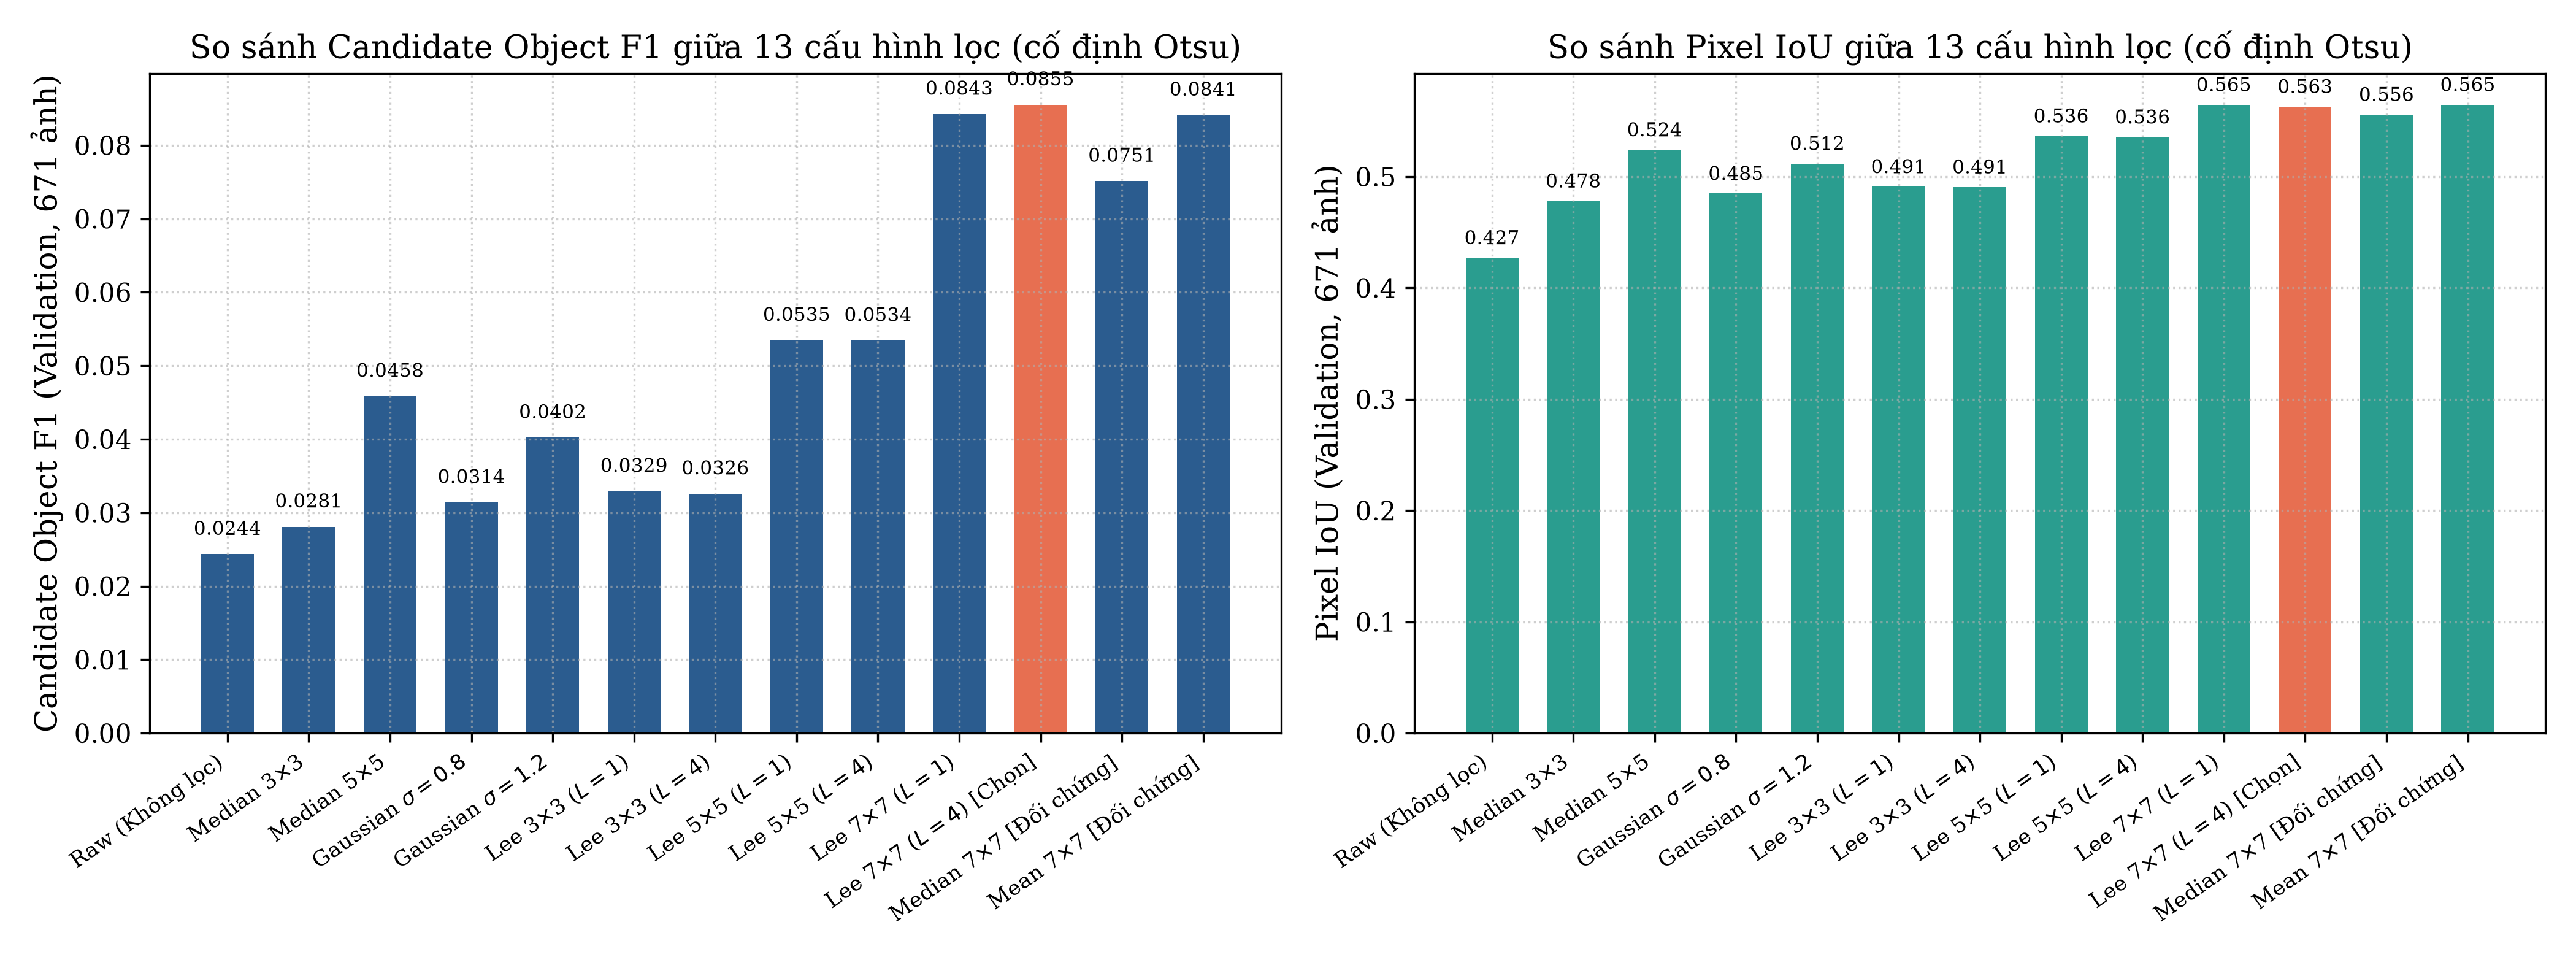
\includegraphics[width=0.96\textwidth]{figures/fig4_filter_threshold_benchmark.png}
\caption{Đối sánh định lượng Candidate Object F1 và Pixel IoU giữa 13 cấu hình lọc không gian (cố định Otsu, $A_{\min}=16$) trên 671 ảnh Validation.}
\label{fig:filter_benchmark_plot}
\end{figure}

\subsection{Phân tích thực nghiệm và hiện tượng suy biến của bộ lọc Lee trên ảnh 8-bit}

Từ Bảng~\ref{tab:filter_benchmark} và Hình~\ref{fig:filter_benchmark_plot}, kết quả thực nghiệm cho thấy 3 phát hiện chính:

\begin{enumerate}
    \item \textbf{Hiệu quả giảm báo nhầm khi mở rộng cửa sổ lọc:}
    Trong dải kích thước cửa sổ $\{3 \times 3, 5 \times 5, 7 \times 7\}$, việc tăng kích thước lên $7 \times 7$ giúp cắt giảm hơn $55\%$ số lượng mảnh nhiễu báo nhầm (từ $>46\,000$ FP xuống còn $\approx 20\,700$ FP), đồng thời nâng Candidate F1 đơn điệu từ $0.0326$ ($3 \times 3$) lên $0.0534$ ($5 \times 5$) và đạt đỉnh $0.0855$ ($7 \times 7$).

    \item \textbf{Hiện tượng suy biến của trọng số Lee về bộ lọc trung bình hộp (mean filter):}
    Cấu hình Lee $7 \times 7$ ($L=4$, F1 $= 0.0855$) đạt chỉ số cao nhất trong không gian quét ban đầu. Tuy nhiên, khi bổ sung phép đối chứng có kiểm soát với bộ lọc trung bình hộp Mean $7 \times 7$ (F1 $= 0.0841$), độ chênh lệch $\Delta\text{F1} = +0.0014$ có khoảng tin cậy Bootstrap 95\% $[-0.0003, +0.0033]$ chứa giá trị 0 (không có ý nghĩa thống kê).
    
    \textit{Giải thích cơ chế:} Do ảnh PNG trong bộ dữ liệu SOS đã qua tiền xử lý làm mượt sơ bộ bởi nhà phát hành, số looks hiệu dụng thực tế trên các vùng biển đồng nhất ($\text{ENL}_{\text{eff}} = m^2 / v$) lớn hơn rất nhiều so với tham số giả định $L \in \{1, 4\}$. Hệ quả là điều kiện $v(x, y) \le m(x, y)^2/L$ xảy ra trên hầu hết các điểm ảnh, khiến trọng số $W(x, y) = 0$ trên diện rộng (như ở hàng 3 Hình~\ref{fig:step_by_step_pipeline} với $\max W = 0.00$) và bộ lọc Lee suy biến về phép lấy trung bình hộp.

    \item \textbf{Sự suy giảm hiệu năng của phân ngưỡng cục bộ Niblack trên biển đồng nhất:}
    Toàn bộ 9 cấu hình Niblack đều ghi nhận hiệu năng thấp (F1 dao động từ $0.0013$ đến $0.0325$, số lượng báo nhầm tăng từ $40\,000$ đến hơn $154\,000$ FP). Nguyên nhân là ở các vùng biển lặng gió có độ biến thiên mức xám rất thấp ($s_W \approx 0$), ngưỡng động $T = m_W - k s_W$ bị hạ thấp và kích hoạt các điểm ảnh ở đuôi phân phối nhiễu thành các đốm tối giả mạo. Vì vậy, phân ngưỡng toàn cục Otsu là giải pháp phù hợp hơn cho bước tạo ứng viên.
\end{enumerate}

\section{Phân tích đặc trưng, nghiên cứu cắt bỏ (ablation) và quá trình hội tụ SVM}
\label{sec:thuc_nghiem_dac_trung_ablation}

\subsection{Thiết kế thí nghiệm quét lưới 729 cấu hình trên tập Validation}

Giữ lại Top-3 cấu hình tạo ứng viên đầu bảng (Lee $7\times 7, L=4$ + Otsu; Lee $7\times 7, L=1$ + Otsu; Lee $5\times 5, L=4$ + Otsu), thực nghiệm quét lưới được tiến hành:
\begin{equation}
3\text{ (lọc/ngưỡng)} \times 3\text{ (hình thái)} \times 3\text{ ($A_{\min}$)} \times 3\text{ (đặc trưng)} \times 9\text{ (mô hình)} = 729\text{ cấu hình}
\end{equation}
trên toàn bộ $671$ ảnh thuộc tập kiểm định (Validation).

\begin{figure}[!htbp]
\centering
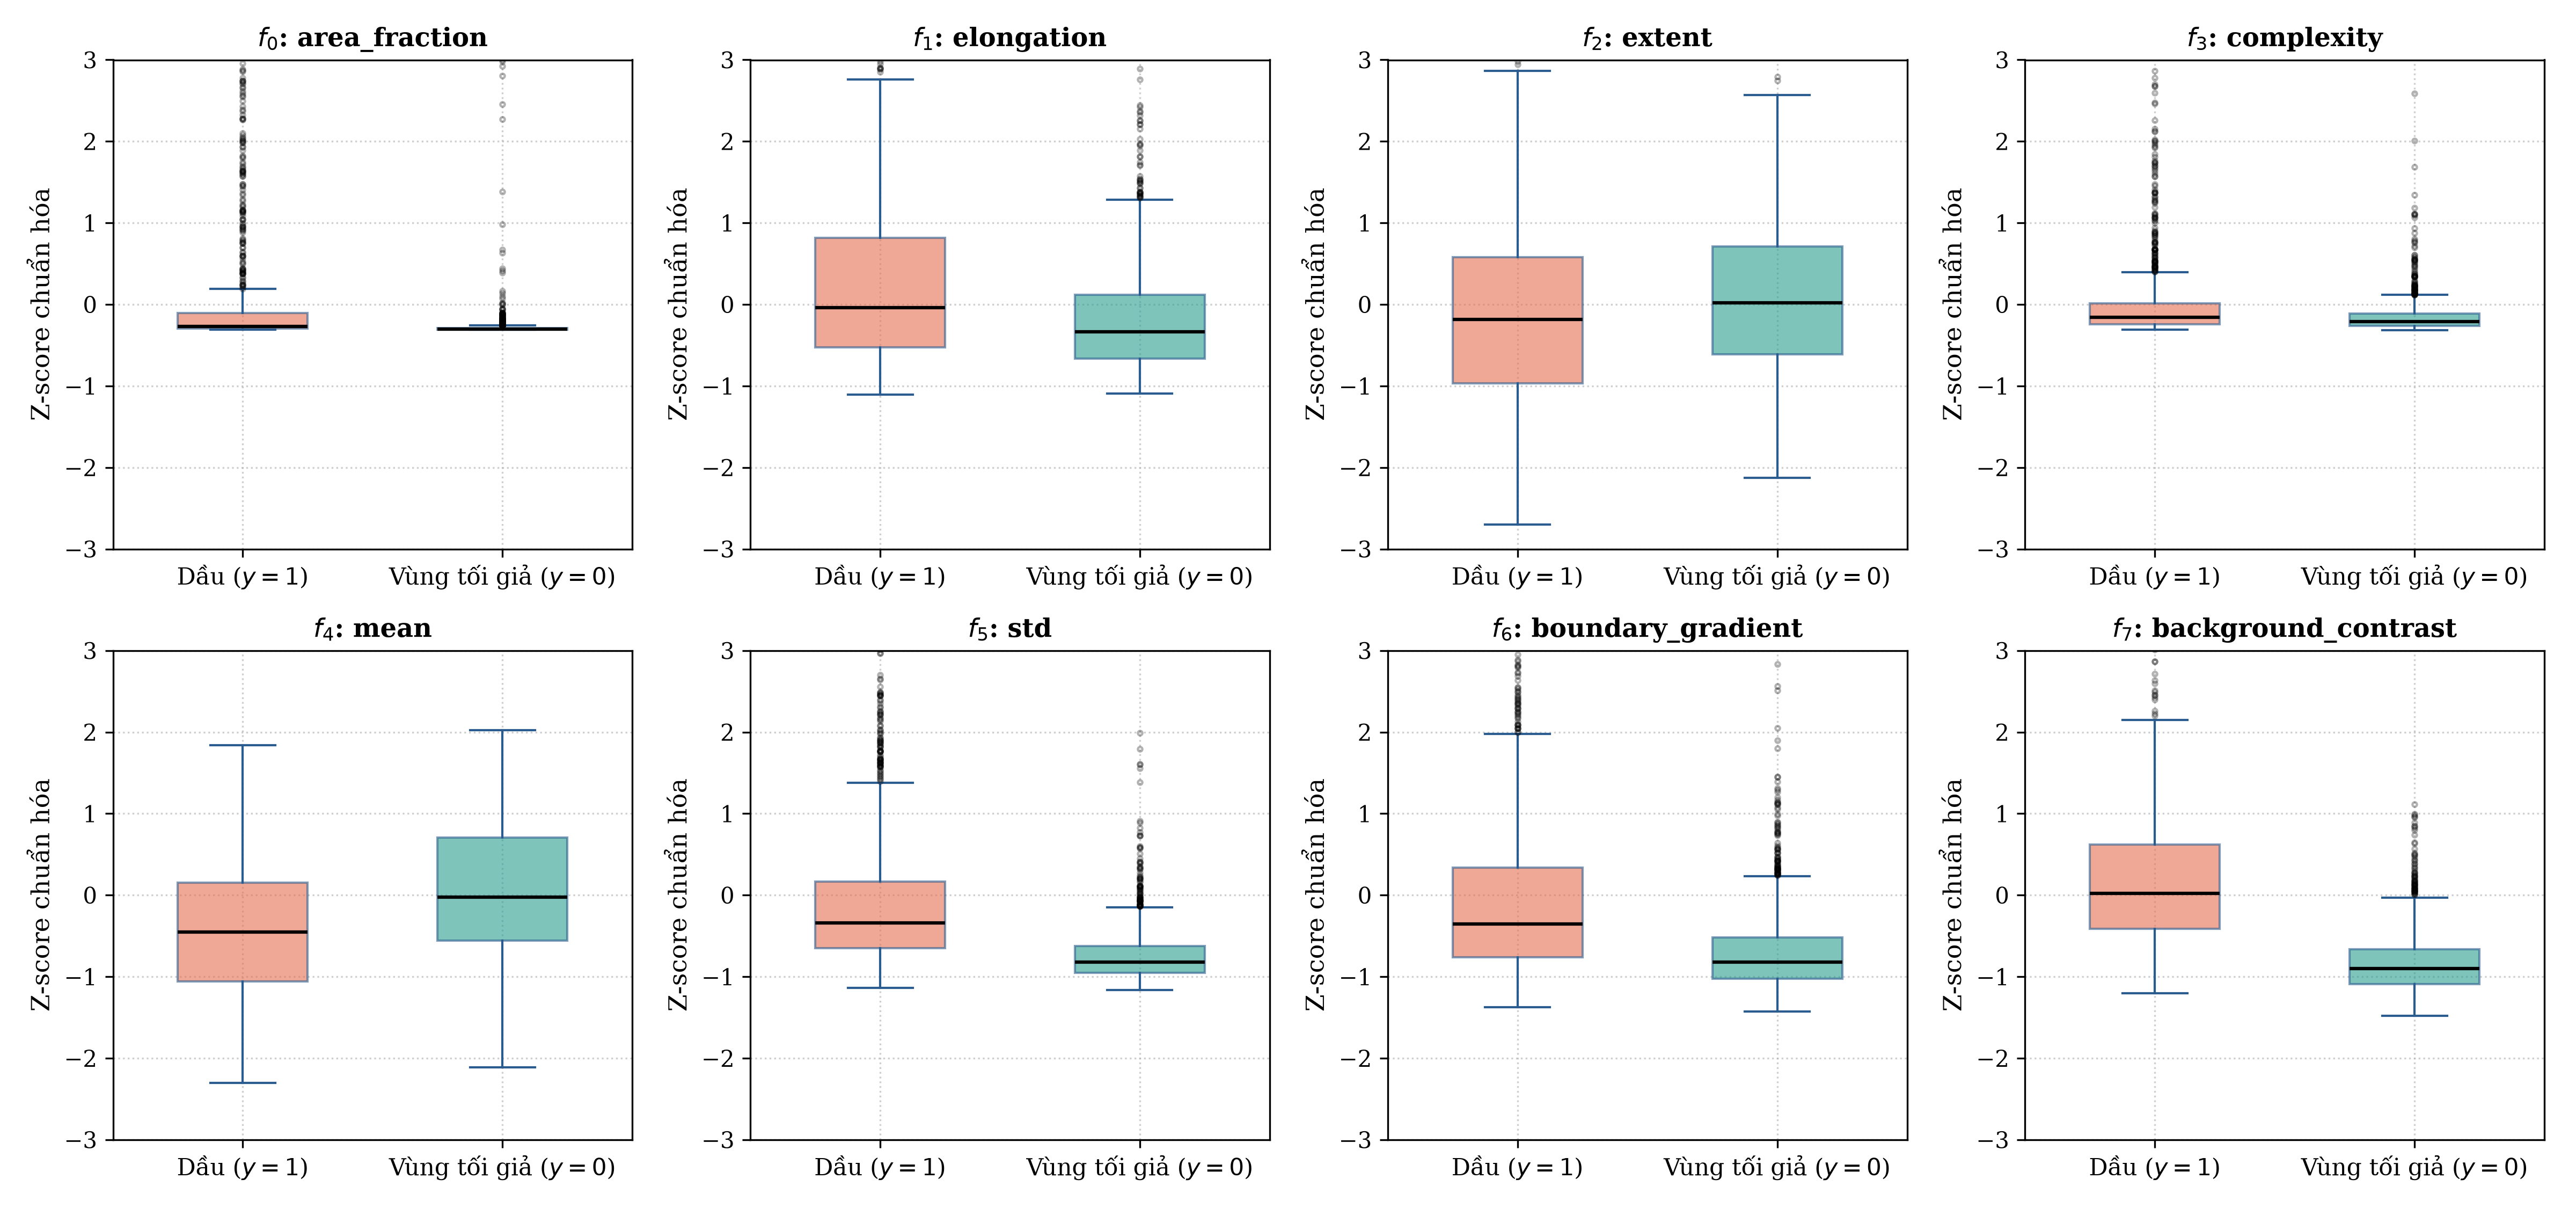
\includegraphics[width=0.98\textwidth]{figures/fig5_feature_distributions.png}
\caption{Biểu đồ Boxplot so sánh phân bố Z-score của 8 đặc trưng vùng giữa lớp Vết dầu thật ($\mathrm{Purity} \ge 0.50$, màu cam) và lớp Vùng tối báo nhầm ($\mathrm{Purity} \le 0.05$, màu xanh ngọc).}
\label{fig:feature_distributions}
\end{figure}

\begin{figure}[!htbp]
\centering
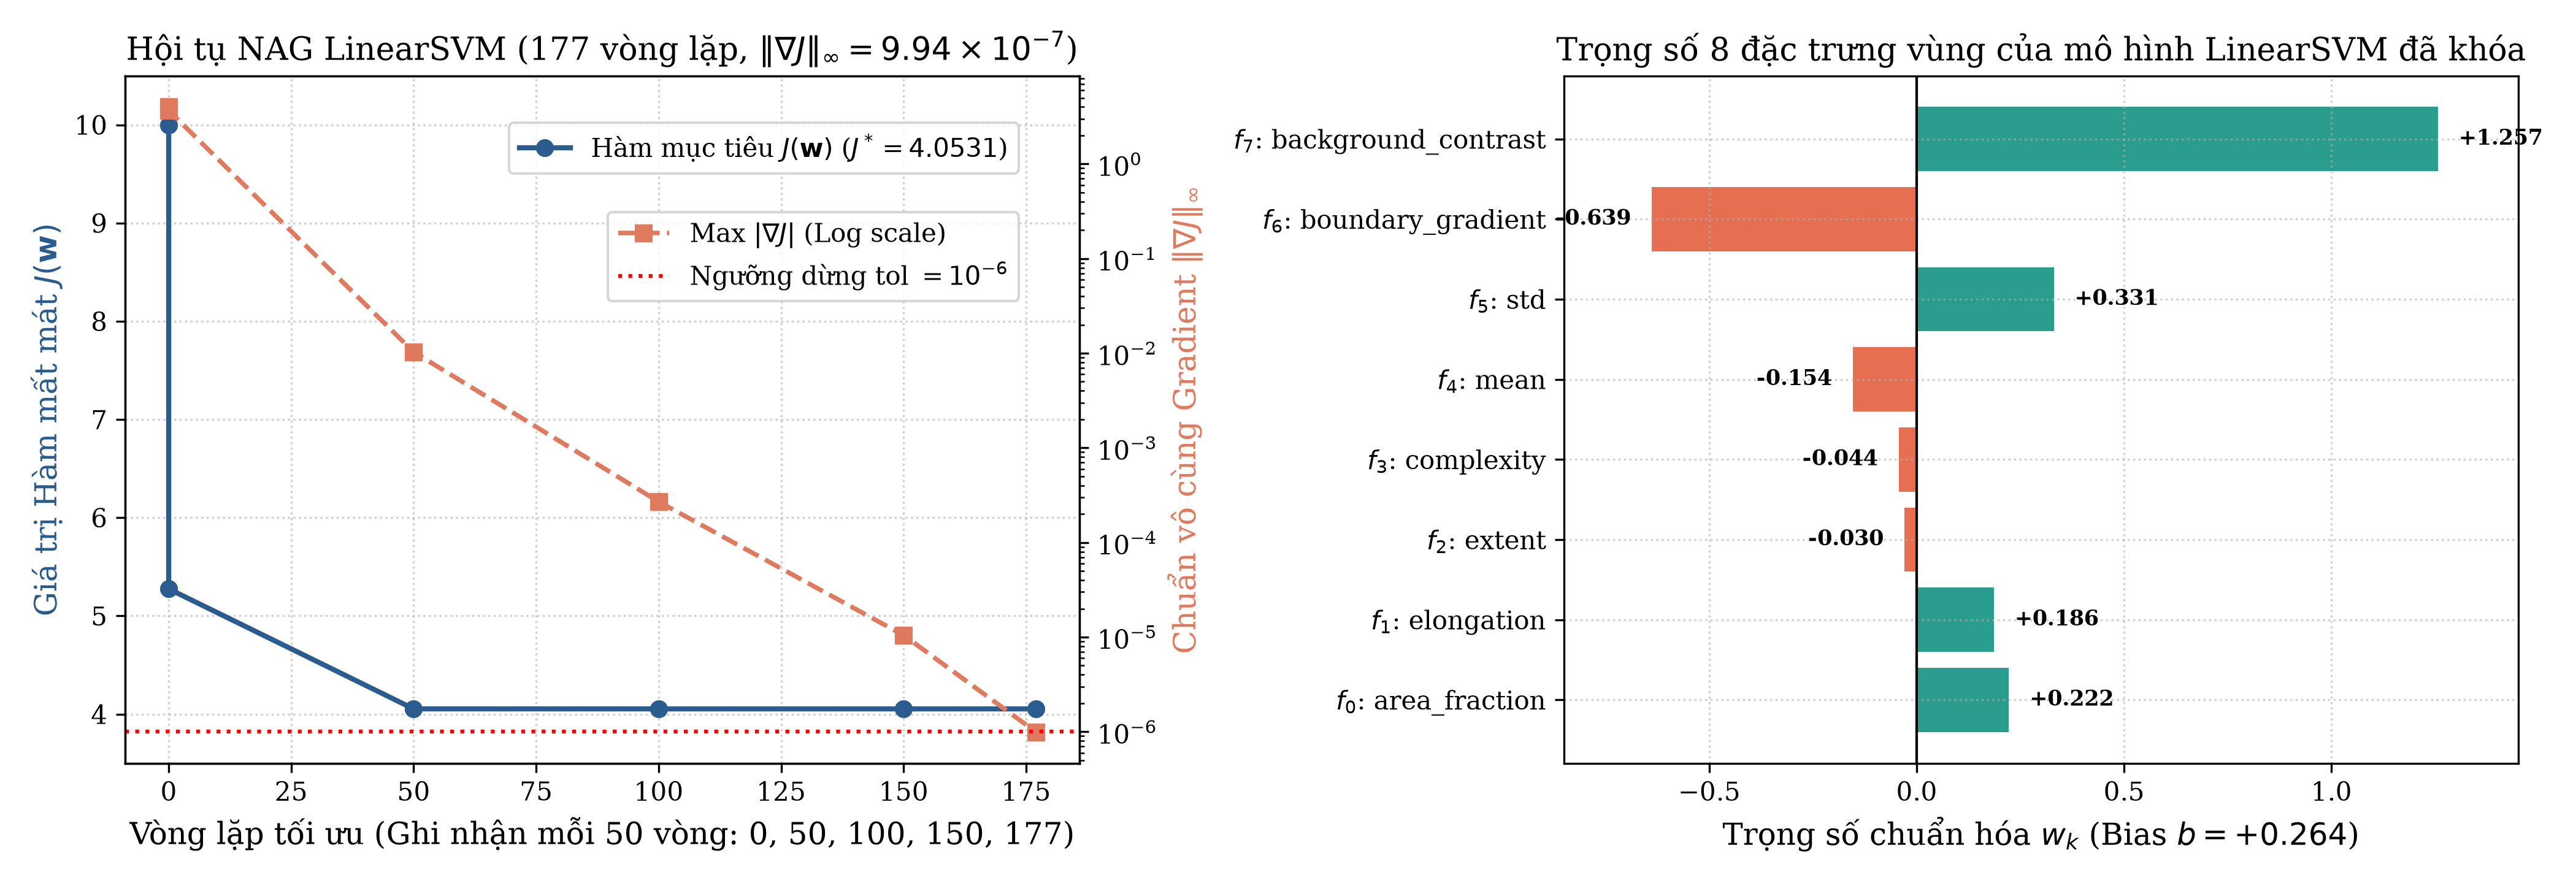
\includegraphics[width=0.96\textwidth]{figures/fig6_svm_convergence_weights.png}
\caption{Đường cong hội tụ của thuật toán tối ưu NAG và biểu đồ trọng số chuẩn hóa $w_k$ của 8 đặc trưng trong mô hình LinearSVM đã khóa.}
\label{fig:svm_convergence_weights}
\end{figure}

Bảng~\ref{tab:ablation_validation} tổng hợp kết quả của nghiên cứu cắt bỏ (Ablation study) nhằm cô lập và bóc tách tác động của từng thành phần kỹ thuật.

\begin{table}[!htbp]
\centering
\small
\caption{Kết quả khảo sát hậu xử lý, nghiên cứu cắt bỏ (Ablation) và so sánh mô hình trên 671 ảnh Validation.}
\label{tab:ablation_validation}
\resizebox{\textwidth}{!}{%
\begin{tabular}{|l|c|c|c|c|c|}
\hline
\textbf{Cấu hình khảo sát} & \textbf{TP} & \textbf{FP} & \textbf{FN} & \textbf{Object F1} & \textbf{Pixel IoU} \\ \hline
\multicolumn{6}{|l|}{\textit{1. Khảo sát ngưỡng diện tích $A_{\min}$ và hình thái học (Lee $7\times 7, L=4$ + Otsu + SVM):}} \\ \hline
$A_{\min} = 4$, \texttt{none} (Không đóng/mở) & $1\,035$ & $8\,571$ & $1\,705$ & 0.1677 & 0.6267 \\ \hline
$A_{\min} = 16$, \texttt{none} (Không đóng/mở) & $1\,034$ & $4\,482$ & $1\,706$ & 0.2505 & 0.6376 \\ \hline
$A_{\min} = 64$, \texttt{none} (\textbf{Cấu hình chọn}) & $\mathbf{1\,016}$ & $2\,215$ & $\mathbf{1\,724}$ & 0.3403 & \textbf{0.6524} \\ \hline
$A_{\min} = 64$, \texttt{close} (Đóng hình thái $3\times 3$) & 971 & $\mathbf{1\,961}$ & $1\,769$ & \textbf{0.3424} & 0.6402 \\ \hline
$A_{\min} = 64$, \texttt{open\_close} (Mở--Đóng $3\times 3$) & 988 & $2\,230$ & $1\,752$ & 0.3317 & 0.6505 \\ \hline
\multicolumn{6}{|l|}{\textit{2. Ablation theo nhóm đặc trưng (LinearSVM, $C=10, A_{\min}=64$, \texttt{none}):}} \\ \hline
Chỉ đặc trưng hình học (\texttt{shape}, 4 chiều) & 736 & $1\,737$ & $2\,004$ & 0.2824 & 0.5899 \\ \hline
Chỉ đặc trưng bức xạ/biên (\texttt{intensity}, 4 chiều) & $1\,002$ & $2\,188$ & $1\,738$ & 0.3379 & \textbf{0.6542} \\ \hline
Kết hợp toàn bộ 8 đặc trưng (\texttt{all}, đề xuất) & $\mathbf{1\,016}$ & $2\,215$ & $\mathbf{1\,724}$ & \textbf{0.3403} & 0.6524 \\ \hline
\multicolumn{6}{|l|}{\textit{3. So sánh mô hình phân loại (Nhóm đặc trưng \texttt{all}, $A_{\min}=64$, \texttt{none}):}} \\ \hline
Cây quyết định CART ($\text{depth}=3, \text{leaf}=20$) & 961 & $\mathbf{1\,998}$ & $1\,779$ & 0.3373 & 0.6456 \\ \hline
LinearSVM ($C=10$, đề xuất) & $\mathbf{1\,016}$ & $2\,215$ & $\mathbf{1\,724}$ & \textbf{0.3403} & \textbf{0.6524} \\ \hline
\multicolumn{6}{|l|}{\textit{4. Đánh giá cấp độ ứng viên theo nhãn Purity ($\mathrm{Purity} \ge 0.50$ vs. $\le 0.05$, $9\,287$ mẫu Val):}} \\ \hline
CART ($\text{TN}=6\,008$, Prec $=0.7952$, Rec $=0.7722$) & $2\,112$ & 544 & 623 & 0.7835 & -- \\ \hline
LinearSVM ($\text{TN}=5\,940$, Prec $=0.7874$, Rec $=0.8285$) & $\mathbf{2\,266}$ & 612 & $\mathbf{469}$ & \textbf{0.8074} & -- \\ \hline
\multicolumn{6}{|l|}{\textit{5. Độ nhạy theo ngưỡng nhị phân Ground Truth (LinearSVM):}} \\ \hline
Ngưỡng mặt nạ GT $M_{\text{raw}} \ge 64$ & $1\,027$ & $2\,204$ & $1\,690$ & 0.3453 & 0.6526 \\ \hline
Ngưỡng mặt nạ GT $M_{\text{raw}} \ge 128$ (Chuẩn) & $1\,016$ & $2\,215$ & $1\,724$ & 0.3403 & 0.6524 \\ \hline
Ngưỡng mặt nạ GT $M_{\text{raw}} \ge 192$ & $1\,010$ & $2\,221$ & $1\,752$ & 0.3371 & 0.6517 \\ \hline
\end{tabular}%
}
\end{table}

\subsection{Phân tích cơ chế biến ức chế và đa cộng tuyến đặc trưng}

Phân tích trọng số của mô hình LinearSVM đã khóa ($\mathbf{w} \in \mathbb{R}^8$ và bias $b = +0.264$ trên Hình~\ref{fig:svm_convergence_weights}) cho thấy cơ chế hoạt động của mô hình:
\begin{itemize}
    \item \textbf{Các đặc trưng quyết định dương tính:} Trọng số dương lớn nhất thuộc về \texttt{background\_contrast} ($w_7 = +1.257$), theo sau là \texttt{std} ($w_5 = +0.331$), \texttt{area\_fraction} ($w_0 = +0.222$) và \texttt{elongation} ($w_1 = +0.186$). Điều này khẳng định độ tương phản bức xạ giữa vùng tối và vành đai nền biển là chỉ dấu quan trọng nhất để xác nhận vết dầu loang.
    \item \textbf{Hiện tượng biến ức chế (suppressor variable) tại $w_6 = -0.639$:}
    Quan sát biểu đồ Boxplot (Hình~\ref{fig:feature_distributions}) cho thấy xét riêng lẻ từng biến (đơn biến), các vết dầu thật có trung vị độ dốc biên \texttt{boundary\_gradient} ($f_6$) cao hơn vùng tối giả, với hệ số tương quan dương $\mathrm{Corr}(f_6, y) = +0.3632$. Tuy nhiên, trong mô hình tuyến tính đa biến, $f_6$ lại nhận trọng số âm $w_6 = -0.639$.
    
    \textit{Nguyên nhân toán học:} Phân tích ma trận tương quan cho thấy $f_6$ có tương quan thuận mạnh với cả độ lệch chuẩn nội vùng $\mathrm{Corr}(f_6, f_5) = +0.8504$ lẫn độ tương phản nền $\mathrm{Corr}(f_6, f_7) = +0.6716$. Khi mô hình đã gán trọng số dương lớn cho $w_7 = +1.257$ và $w_5 = +0.331$, đặc trưng $f_6$ đóng vai trò là một \textit{biến ức chế}: trọng số âm $w_6 = -0.639$ giúp khử phần phương sai nhiễu dư thừa của các vùng có đạo hàm biên gắt do cắt ngưỡng hoặc nhiễu cục bộ nhưng lại thiếu sự chênh lệch mức xám nền tương xứng.
\end{itemize}

\section{Đánh giá định lượng và định tính trên tập kiểm thử độc lập}
\label{sec:danh_gia_test_phan_tang}

\subsection{Đánh giá so sánh định lượng trên tập kiểm thử độc lập}

Sau khi đóng băng cấu hình được chọn trên tập Validation, đánh giá được thực hiện trên tập kiểm thử độc lập gồm \textbf{839 ảnh Sentinel-1A} (chứa tổng cộng $3\,182$ đối tượng dầu Ground Truth) và tập kiểm thử ngoài cảm biến gồm \textbf{776 ảnh ALOS PALSAR} (chứa $3\,994$ đối tượng dầu Ground Truth).

Bảng~\ref{tab:model_comparison} trình bày chi tiết kết quả định lượng tổng hợp, gồm cả cách tính Micro-averaging và Macro-averaging ($\text{mean} \pm \text{SD}$ giữa các ảnh).

\begin{table}[!htbp]
\centering
\caption{Đánh giá so sánh hiệu năng trên tập kiểm thử độc lập (839 ảnh Sentinel-1A và 776 ảnh ALOS PALSAR) theo giao thức ghép cặp Hungarian ở ngưỡng $\IoU \ge 0.5$.}
\label{tab:model_comparison}
\begingroup
\setlength{\tabcolsep}{2pt}
\renewcommand{\arraystretch}{1.2}
\resizebox{\textwidth}{!}{%
\begin{tabular}{|>{\raggedright\arraybackslash}p{3.2cm}|c|*{9}{>{\centering\arraybackslash}p{1.82cm}|}}
\hline
\textbf{Phương pháp} & \textbf{Ảnh} & \textbf{TP} & \textbf{FP} & \textbf{FN} & \textbf{Prec} & \textbf{Rec} & \textbf{Obj F1} & \textbf{Pix IoU} & \textbf{FP/ảnh} & \begin{tabular}{@{}c@{}}\textbf{Edge / Int}\\\textbf{Recall}\end{tabular} \\ \hline
\textit{Baseline (Ảnh thô + Otsu, $A_{\min} = 16$)} & 839 & 426 & $49\,182$ & $2\,756$ & 0.0086 & 0.1339 & 0.0161 & 0.4367 & 58.62 & 0.1979 / 0.0038 \\ \hline
\textit{Lee 7$\times$7 + Otsu ($A_{\min} = 64$, Không Clf)} & 839 & $1\,018$ & $12\,495$ & $2\,164$ & 0.0753 & \textbf{0.3199} & 0.1220 & 0.5867 & 14.89 & \textbf{0.4221} / \textbf{0.1124} \\ \hline
\textbf{Pipeline + LinearSVM ($A_{\min} = 64$, Đề xuất)} & 839 & 996 & $\mathbf{2\,923}$ & $2\,186$ & \textbf{0.2541} & 0.3130 & \textbf{0.2805} & \textbf{0.6614} & \textbf{3.48} & 0.4156 / 0.1048 \\ \hline
\quad \textit{Macro từng ảnh ($\text{mean} \pm \text{SD}$)$^{\dagger}$} & \multicolumn{4}{c|}{--} & $0.356 \pm 0.336$ & $0.446 \pm 0.382$ & $0.349 \pm 0.317$ & $0.577 \pm 0.261$ & $3.48 \pm 3.97$ & -- \\ \hline
\textit{Ngoài cảm biến: PALSAR (LinearSVM, $A_{\min} = 64$)} & 776 & $1\,441$ & $2\,305$ & $2\,553$ & 0.3847 & 0.3608 & 0.3724 & 0.6423 & 2.97 & 0.4587 / 0.1890 \\ \hline
\quad \textit{Macro từng ảnh ($\text{mean} \pm \text{SD}$)$^{\ddagger}$} & \multicolumn{4}{c|}{--} & $0.465 \pm 0.342$ & $0.438 \pm 0.338$ & $0.412 \pm 0.312$ & $0.579 \pm 0.234$ & $2.97 \pm 3.43$ & -- \\ \hline
\end{tabular}%
}
\par\vspace{3pt}
{\raggedright\footnotesize
$^{\dagger}$Cỡ mẫu xác định trên Sentinel-1A (839 ảnh): $n_{\text{Prec}}=786$, $n_{\text{Rec}}=808$, $n_{\text{F1}}=n_{\text{IoU}}=814$ (25 ảnh $R_0$ có $\text{TP}=\text{FP}=\text{FN}=0$).\par
$^{\ddagger}$Cỡ mẫu xác định trên ALOS PALSAR (776 ảnh): $n_{\text{Prec}}=705$, $n_{\text{Rec}}=731$, $n_{\text{F1}}=n_{\text{IoU}}=734$ (42 ảnh $R_0$ có $\text{TP}=\text{FP}=\text{FN}=0$).\par}
\endgroup
\end{table}

\begin{figure}[!htbp]
\centering
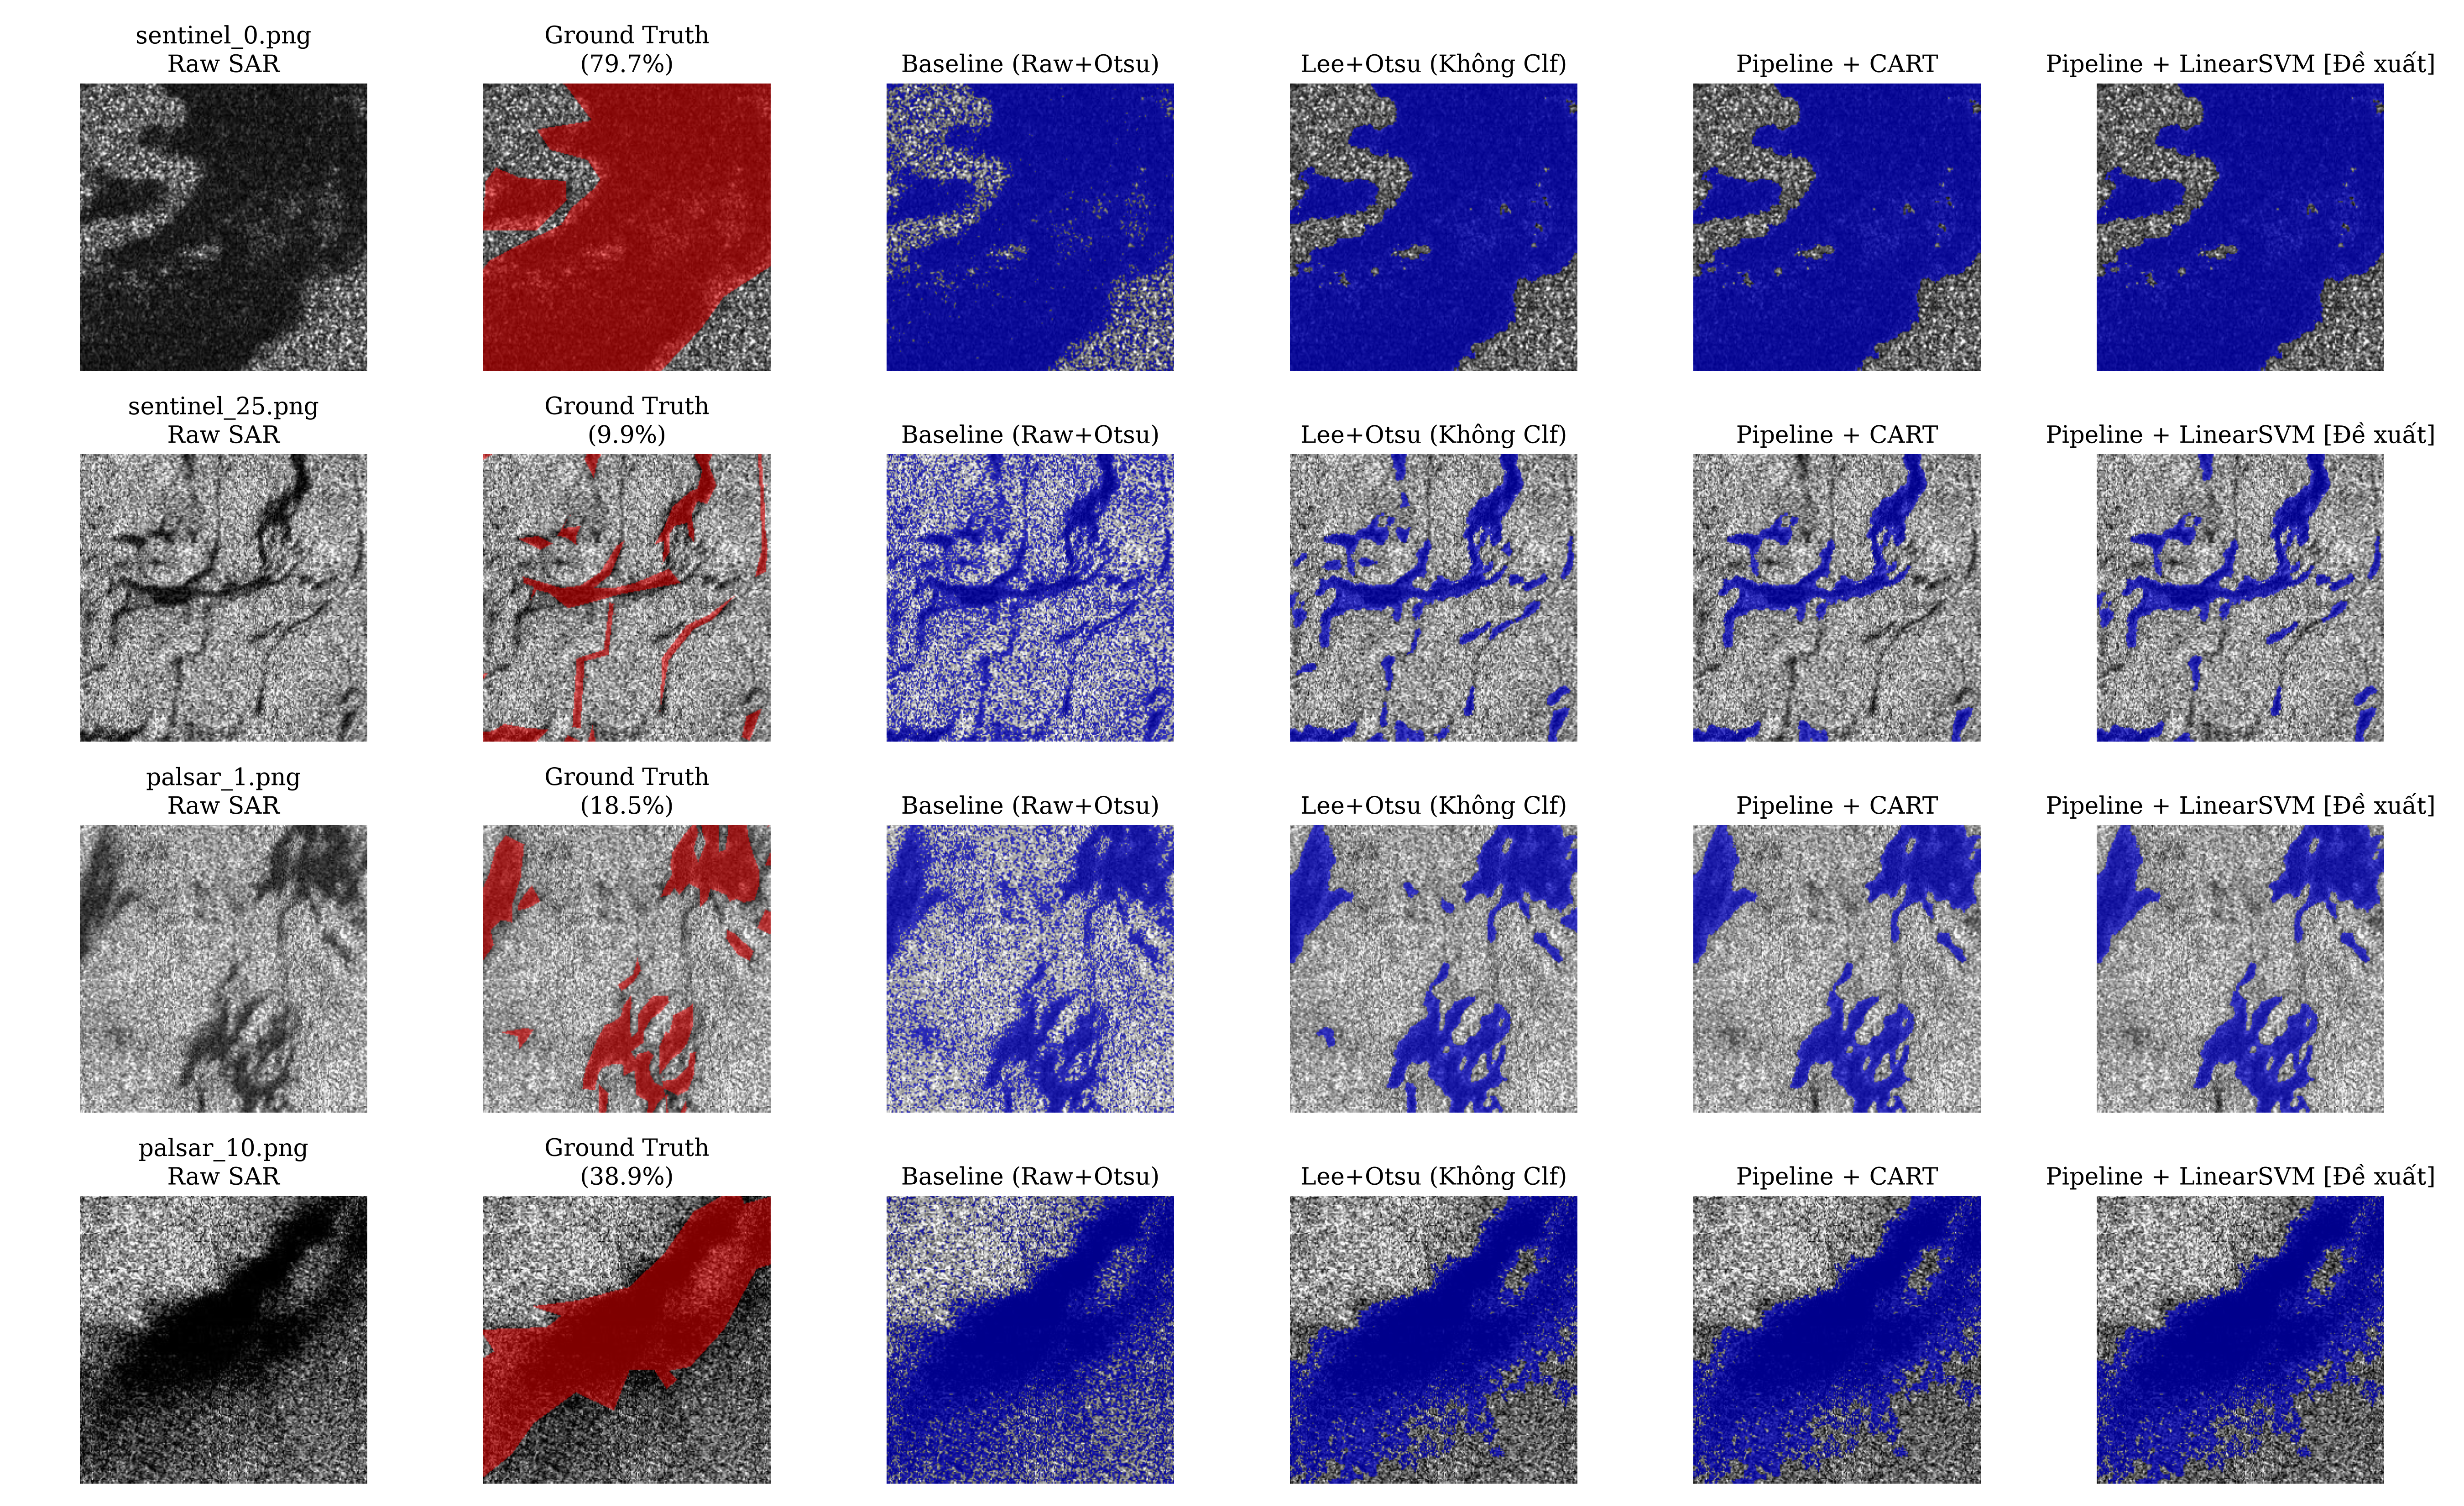
\includegraphics[width=\textwidth]{figures/fig7_qualitative_comparison.png}
\caption{Đối sánh định tính kết quả phân đoạn giữa các phương pháp trên 4 cảnh SAR viễn thám đại diện: Cột 1: Ảnh gốc; Cột 2: Mặt nạ Ground Truth; Cột 3: Baseline thô; Cột 4: Lọc Lee + Otsu (Không classifier); Cột 5: Pipeline + CART; Cột 6: Pipeline + LinearSVM (Đề xuất).}
\label{fig:qualitative_comparison}
\end{figure}

Hình~\ref{fig:qualitative_comparison} minh họa đối sánh định tính trên 4 cảnh SAR điển hình. Kết quả định lượng cho thấy:
\begin{enumerate}
    \item \textbf{Cắt giảm $76.6\%$ số vùng báo nhầm:} So với cấu hình tạo ứng viên không dùng classifier ($\text{TP}=1\,018, \text{FP}=12\,495$), việc tích hợp bộ phân loại LinearSVM đã loại bỏ $9\,572$ vùng tối giả, đưa tỷ lệ cảnh báo sai từ $14.89$ xuống còn $3.48$ FP/ảnh.
    \item \textbf{Bảo toàn $97.8\%$ số đối tượng đúng:} LinearSVM giữ lại $996 / 1\,018$ TP của giai đoạn ứng viên (chỉ giảm 22 đối tượng), nâng Precision lên $3.37$ lần (từ $0.0753$ lên $0.2541$), nâng Object F1 từ $0.1220$ lên $0.2805$ ($\Delta\text{F1} = +0.1586$, 95\% CI $[+0.1474, +0.1706]$) và Pixel IoU đạt $0.6614$.
\end{enumerate}

\subsection{Hiệu năng phân tầng theo 5 chế độ diện tích và khả năng chuyển giao ngoài cảm biến}

Bảng~\ref{tab:regime_breakdown} và Hình~\ref{fig:regime_sensor} phân tích chi tiết hiệu năng của hệ thống theo từng lát cắt dữ liệu vật lý ($R_0 \to R_4$) trên cả hai cảm biến Sentinel-1A và ALOS PALSAR.

\begin{figure}[!htbp]
\centering
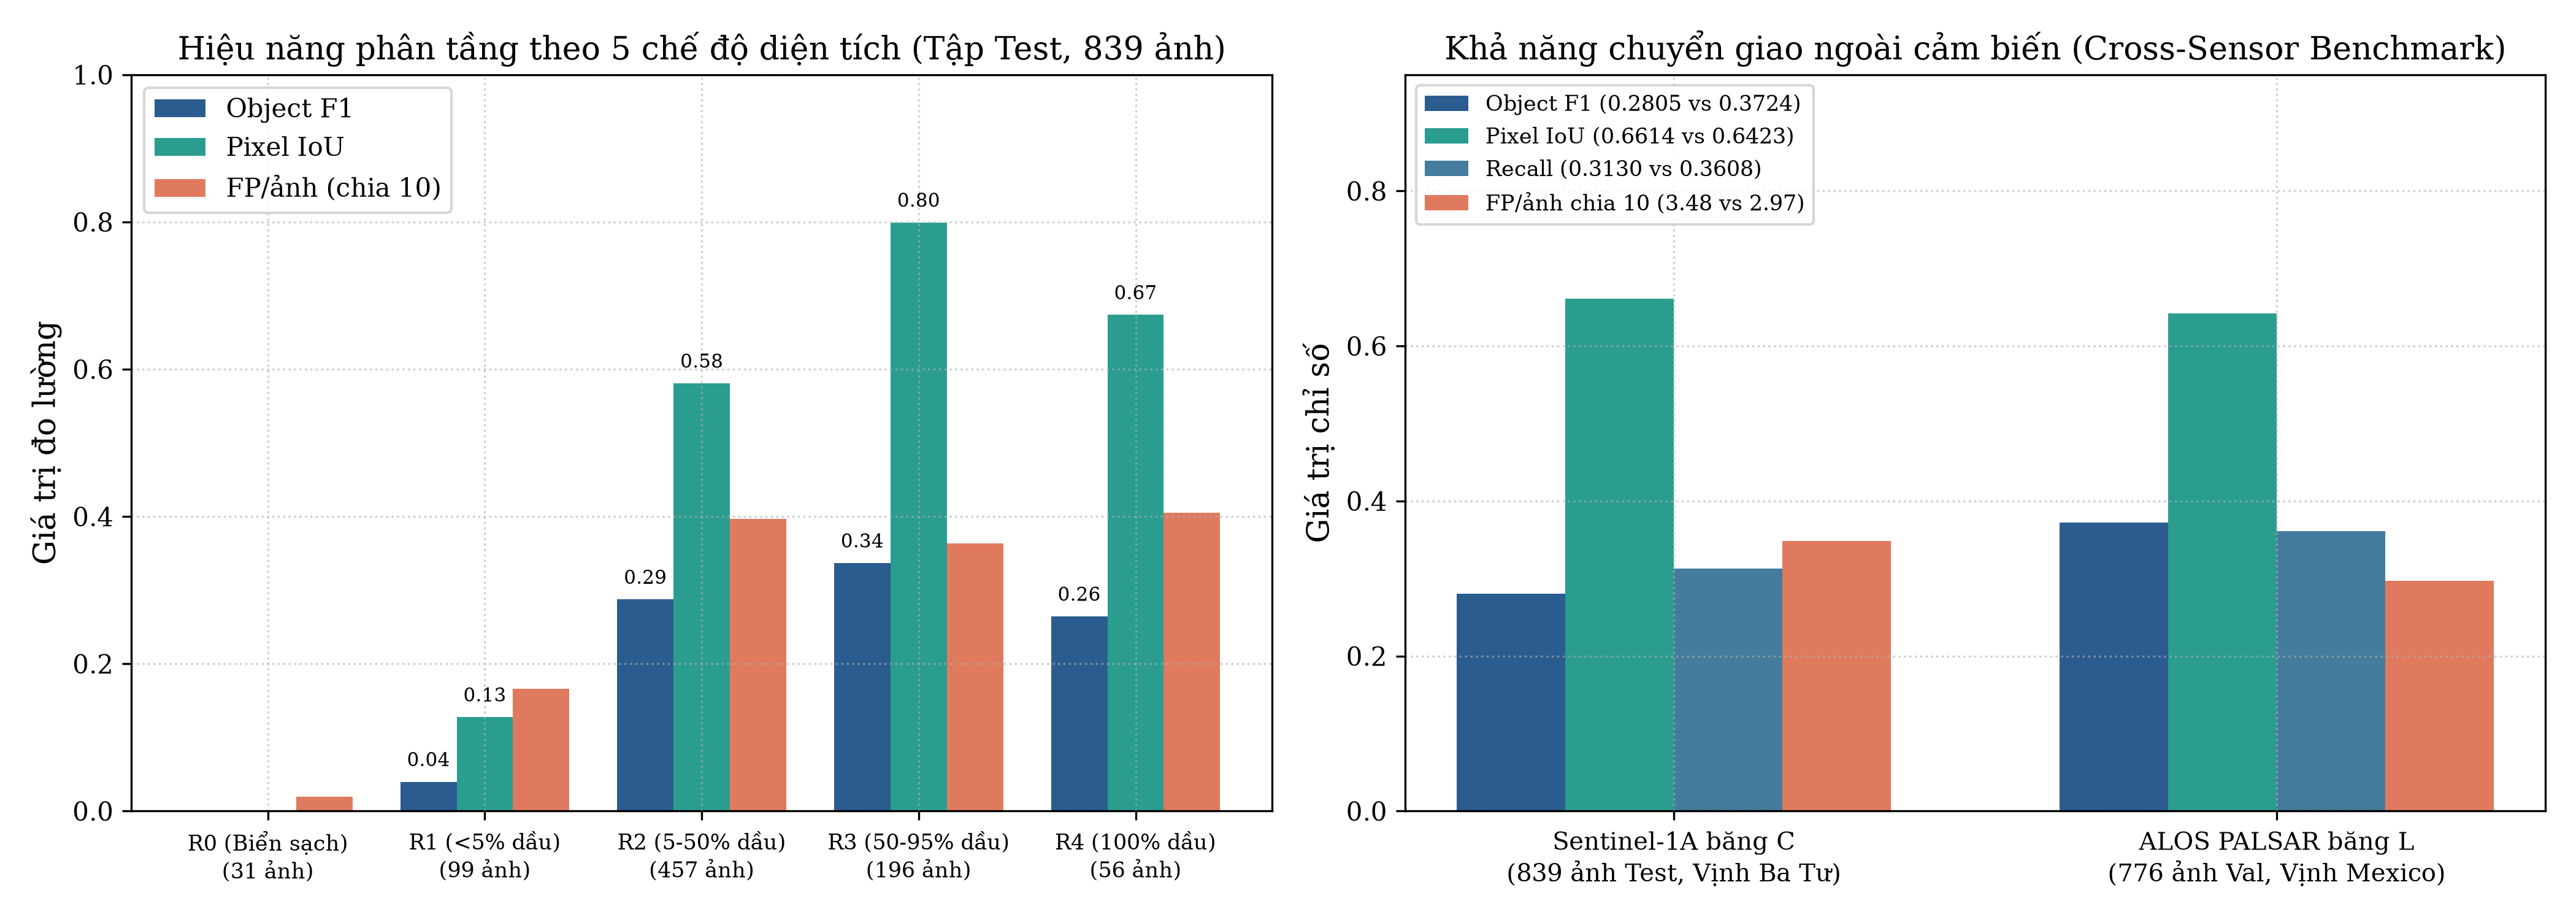
\includegraphics[width=0.96\textwidth]{figures/fig8_regime_sensor_performance.png}
\caption{Hiệu năng phân tầng theo 5 chế độ diện tích dầu ($R_0 \to R_4$) trên 839 ảnh Test Sentinel-1A (trái) và chuyển giao sang 776 ảnh ALOS PALSAR (phải).}
\label{fig:regime_sensor}
\end{figure}

\begin{table}[!htbp]
\centering
\small
\caption{Chi tiết hiệu năng phân tầng theo 5 chế độ diện tích dầu ($R_0 \to R_4$) trên hai tập kiểm thử độc lập.}
\label{tab:regime_breakdown}
\resizebox{\textwidth}{!}{%
\begin{tabular}{|l|c|c|c|c|c|c|c|}
\hline
\textbf{Chế độ diện tích} & \textbf{Số ảnh} & \textbf{TP} & \textbf{FP} & \textbf{FN} & \textbf{Object F1} & \textbf{Pixel IoU} & \textbf{FP / ảnh} \\ \hline
\multicolumn{8}{|l|}{\textit{Tập kiểm thử Sentinel-1A (839 ảnh, Vịnh Ba Tư, băng C, VV):}} \\ \hline
$R_0$ (Biển sạch, 0\% dầu) & 31 & 0 & 6 & 0 & N/A & N/A & \textbf{0.19} \\ \hline
$R_1$ (Vết dầu nhỏ, $<5\%$) & 99 & 9 & 164 & 271 & 0.0397 & 0.1276 & 1.66 \\ \hline
$R_2$ (Dải dầu trung bình, $5\text{--}50\%$) & 457 & 693 & $1\,814$ & $1\,624$ & 0.2873 & 0.5808 & 3.97 \\ \hline
$R_3$ (Dầu diện rộng, $50\text{--}95\%$) & 196 & 250 & 712 & 273 & \textbf{0.3367} & \textbf{0.7993} & 3.63 \\ \hline
$R_4$ (Ngập dầu toàn phần, $\ge 95\%$) & 56 & 44 & 227 & 18 & 0.2643 & 0.6738 & 4.05 \\ \hline
\textbf{Tổng hợp Sentinel-1A} & \textbf{839} & \textbf{996} & $\mathbf{2\,923}$ & $\mathbf{2\,186}$ & \textbf{0.2805} & \textbf{0.6614} & \textbf{3.48} \\ \hline
\multicolumn{8}{|l|}{\textit{Tập kiểm thử ngoài cảm biến ALOS PALSAR (776 ảnh, Vịnh Mexico, băng L, HH):}} \\ \hline
$R_0$ (Biển sạch, 0\% dầu) & 45 & 0 & 3 & 0 & N/A & N/A & \textbf{0.07} \\ \hline
$R_1$ (Vết dầu nhỏ, $<5\%$) & 113 & 36 & 223 & 359 & 0.1101 & 0.2274 & 1.97 \\ \hline
$R_2$ (Dải dầu trung bình, $5\text{--}50\%$) & 585 & $1\,360$ & $2\,034$ & $2\,165$ & 0.3931 & 0.6480 & 3.48 \\ \hline
$R_3$ (Dầu diện rộng, $50\text{--}95\%$) & 31 & 43 & 45 & 29 & 0.5375 & 0.8153 & 1.45 \\ \hline
$R_4$ (Ngập dầu toàn phần, $\ge 95\%$) & 2 & 2 & 0 & 0 & \textbf{1.0000} & \textbf{0.8827} & \textbf{0.00} \\ \hline
\textbf{Tổng hợp ALOS PALSAR} & \textbf{776} & $\mathbf{1\,441}$ & $\mathbf{2\,305}$ & $\mathbf{2\,553}$ & \textbf{0.3724} & \textbf{0.6423} & \textbf{2.97} \\ \hline
\end{tabular}%
}
\end{table}

\subsection{Phân tích sự khác biệt giữa độ chính xác phân loại theo độ tinh khiết và chỉ số Hungarian IoU}

Thực nghiệm cho thấy sự khác biệt có tính phương pháp luận giữa độ chính xác của bộ phân loại theo nhãn độ tinh khiết ($\text{F1} = 80.74\%$) và chỉ số Object F1 cuối cùng ($0.2805$):
\begin{itemize}
    \item Đối chiếu kết quả trên tập Validation cho thấy: trong số $2\,878$ vùng được LinearSVM dự đoán dương tính, chỉ có \textbf{$612$ vùng ($21.3\%$) là báo nhầm nền biển sạch thực sự} ($\mathrm{Purity} \le 0.05$).
    \item Ngược lại, có tới \textbf{$2\,266$ vùng dự đoán dương tính thực sự nằm đè lên vệt dầu thật} ($\mathrm{Purity} \ge 0.50$), nhưng chỉ có $1\,016$ vùng trong số đó vượt qua ngưỡng ghép cặp một-một $\IoU \ge 0.50$ để trở thành TP đối tượng.
    \item Hơn \textbf{$1\,250$ mảnh dầu thật còn lại bị giao thức Hungarian tính là FP đối tượng} (chiếm $56.4\%$ tổng số FP). Điều này cho thấy phần lớn cảnh báo sai ở cấp đối tượng không phải do mô hình nhận nhầm nước biển thành dầu, mà là do vết dầu lớn bị bước phân ngưỡng Otsu cắt vụn thành nhiều mảnh con.
\end{itemize}

\section{Phân tích trường hợp thất bại và thời gian tính toán}
\label{sec:that_bai_thoi_gian}

\subsection{Phân tích ba trường hợp thất bại cực đoan điển hình}

Nhằm xác định rõ giới hạn của phương pháp xử lý ảnh truyền thống, 3 ca thất bại tiêu biểu được phân tích chi tiết:

\begin{enumerate}
    \item \textbf{Ca nhiều cảnh báo sai (FP) đối tượng nhất --- Ảnh \texttt{val/sentinel\_440.png} (Chế độ $R_4$ ngập $100\%$ dầu):}
    Do toàn bộ khung ảnh nằm trọn trong mảng dầu khổng lồ, biểu đồ histogram có dạng đơn đỉnh hẹp. Thuật toán Otsu toàn cục buộc phải chia đôi chính mảng dầu thành $35$ mảnh ứng viên nhỏ. Mặc dù toàn bộ 35 mảnh này đều có độ tinh khiết $\mathrm{Purity} = 1.00$ (nằm hoàn toàn trên dầu thật), diện tích của từng mảnh riêng lẻ đều quá nhỏ so với mặt nạ Ground Truth nguyên khối duy nhất, dẫn đến không mảnh nào đạt $\IoU \ge 0.5$. Hệ quả là hệ thống nhận $0$ TP, $35$ FP và $1$ FN đối tượng.

    \item \textbf{Ca bỏ sót (FN) đối tượng nhiều nhất --- Ảnh \texttt{val/sentinel\_25.png} (Chế độ $R_2$):}
    Cảnh chụp chứa các dải dầu mảnh hẹp, đứt đoạn có độ tương phản mức xám yếu so với nền biển. Ngưỡng Otsu toàn cục bị nâng lên quá cao bởi diện tích nền biển sáng rộng lớn, khiến các dải dầu mảnh bị xóa nhòa ngay từ Giai đoạn 1 (tạo ứng viên), gây ra $20$ FN đối tượng. Điều này giải thích vì sao chỉ số \texttt{Interior Recall} của hệ thống chỉ đạt $10.48\%$.

    \item \textbf{Ca tổng điểm ảnh sai lớn nhất --- Ảnh \texttt{val/sentinel\_591.png} (Chế độ $R_3$):}
    Mảng dầu diện rộng bao phủ hơn $70\%$ khung ảnh. Bước phân ngưỡng ban đầu làm mất hơn $38\,000$ điểm ảnh dầu do phân bố mức xám không đều. Tiếp đó, do mảng dầu quá lớn làm rỗng vành đai nền 5 pixel ngoài biên, thuật toán chuyển sang cơ chế fallback tính $\mu_{\text{bg}}$ trên phần điểm ảnh sáng còn lại của mảng dầu, làm sai lệch hoàn toàn đặc trưng tương phản nền $f_7$ và khiến bộ phân loại bác bỏ nhầm toàn bộ các ứng viên dầu thật.
\end{enumerate}

\subsection{Đánh giá thời gian chạy thực tế và hiệu năng tính toán trên CPU}

Bảng~\ref{tab:thoi_gian_chay} so sánh thời gian thực thi trung bình trên mỗi ảnh $256 \times 256$ đo lường qua thực thi song song 4 tiến trình worker trên toàn bộ 839 ảnh Test.

\begin{table}[!htbp]
\centering
\small
\caption{Thời gian thực thi trung bình và tổng thời gian xử lý 839 ảnh Test trên CPU.}
\label{tab:thoi_gian_chay}
\resizebox{\textwidth}{!}{%
\begin{tabular}{|l|c|c|c|}
\hline
\textbf{Cấu hình phương pháp} & \textbf{Thời gian trung bình / ảnh} & \textbf{Tổng thời gian} & \textbf{Tốc độ thông lượng} \\ \hline
\textit{Baseline thô (Không lọc + Otsu)} & $107.8 \pm 34.2\text{ ms}$ & $90.46\text{ giây}$ & $\sim 9.3\text{ ảnh/giây}$ \\ \hline
\textbf{Pipeline đầy đủ + LinearSVM} & $\mathbf{50.2 \pm 14.7\text{ ms}}$ & $\mathbf{42.11\text{ giây}}$ & $\mathbf{\sim 19.9\text{ ảnh/giây}}$ \\ \hline
\end{tabular}%
}
\end{table}

\noindent\textbf{So sánh tốc độ giữa pipeline đề xuất và baseline không lọc:}
Dù thực hiện thêm lọc Lee $7 \times 7$, trích xuất 8 đặc trưng và suy luận LinearSVM, thời gian xử lý trung bình của pipeline đầy đủ giảm từ $107.8\text{ ms}$ xuống $50.2\text{ ms/ảnh}$. Ở cấu hình không lọc, nhiễu đốm khiến Otsu sinh ra $49\,608$ mảnh nhiễu li ti làm chậm bước gán nhãn liên thông và trích xuất vùng; ngược lại, lọc Lee $7 \times 7$ kết hợp ngưỡng $A_{\min} = 64$ đã loại bỏ hơn $72\%$ mảnh vụn, thu gọn số vùng liên thông cần xử lý xuống còn $13\,513$ vùng trên toàn tập ảnh và tăng tốc độ xử lý gần 2 lần.


% CHƯƠNG 5: KẾT LUẬN VÀ HƯỚNG PHÁT TRIỂN
\chapter{Kết luận và hướng phát triển}
\label{chap:ket_luan}
\section{Đối chiếu mục tiêu đề tài và kết quả thực tế đạt được}
\label{sec:doi_chieu_muc_tieu}

Nhằm tổng kết đánh giá kết quả thực hiện, Bảng~\ref{tab:doi_chieu_muc_tieu} đối chiếu chi tiết từng mục tiêu đề ra tại Chương 1 và các yêu cầu chức năng của đề tài với kết quả thực tế đo đạc được trên hệ thống.

\begin{table}[!htbp]
\centering
\small
\caption{Bảng đối chiếu từng mục tiêu ban đầu với kết quả thực tế đạt được trong bài tập lớn.}
\label{tab:doi_chieu_muc_tieu}
\resizebox{\textwidth}{!}{%
\begin{tabular}{|p{4.0cm}|c|p{7.5cm}|}
\hline
\textbf{Mục tiêu đề ra tại Chương 1} & \textbf{Tình trạng} & \textbf{Bằng chứng số liệu và kết quả thực tế} \\ \hline
\textbf{1. Tự cài đặt các thuật toán cốt lõi bằng NumPy thuần} & \textbf{Đạt} & Toàn bộ 6 khối chức năng được tự viết trong \texttt{core.py} và \texttt{models.py}; kiểm chứng 118 ca biên và 192 phép toán thực tế trên ảnh SOS đạt $\max |\Delta| < 1.4 \times 10^{-11}$. \\ \hline
\textbf{2. Kiểm chứng bộ phân loại học máy với scikit-learn} & \textbf{Đạt} & Cả LinearSVM và CART tự cài đặt đều đạt độ đồng thuận dự đoán 100\% ($\text{Agreement} = 1.0000$); độ lệch hàm mục tiêu tối ưu đạt $2.88 \times 10^{-12}$. \\ \hline
\textbf{3. Cắt giảm trên 70\% số lượng vùng tối báo nhầm} & \textbf{Đạt} & LinearSVM cắt giảm $76.6\%$ số vùng báo nhầm trên tập Test (từ $14.89$ xuống $3.48$ FP/ảnh), giảm $99.2\%$ báo nhầm trên ảnh biển sạch $R_0$ (từ $24.32$ xuống $0.19$ FP/ảnh). \\ \hline
\textbf{4. Bảo toàn trên 95\% số đối tượng đúng của giai đoạn 1} & \textbf{Đạt} & Mô hình giữ lại được $97.8\%$ số đối tượng đúng do bước tạo ứng viên đề xuất ($996/1\,018$ TP), chỉ làm mất 22 đối tượng. \\ \hline
\textbf{5. Đạt độ bao phủ điểm ảnh $\text{Pixel IoU} \ge 0.60$} & \textbf{Đạt} & Đạt Global Pixel IoU $= 0.6614$ trên tập Test độc lập Sentinel-1A và $0.6423$ trên tập ALOS PALSAR. \\ \hline
\textbf{6. Đánh giá khách quan chuẩn ghép cặp Hungarian} & \textbf{Đạt} & Thiết lập thuật toán Hungarian ở ngưỡng $\IoU \ge 0.5$, ghi nhận Object F1 $= 0.2805$ trên 839 ảnh Test Sentinel-1A và $0.3724$ trên 776 ảnh ALOS PALSAR. \\ \hline
\textbf{7. Chuẩn hóa góc tới và ghép trường gió} & \textit{Chưa đạt} & Bộ dữ liệu Refined SOS dạng ảnh PNG cắt sẵn thiếu siêu dữ liệu góc tới và dấu thời gian/tọa độ để ghép dữ liệu gió ECMWF ERA5. \\ \hline
\textbf{8. Phân biệt riêng các loại tương tự dầu (look-alikes)} & \textit{Chưa đạt} & Mặt nạ tham chiếu SOS chỉ có nhãn nhị phân dầu/nền, chưa có nhãn phân tách riêng cho màng sinh học, vùng lặng gió hay bóng mưa. \\ \hline
\end{tabular}%
}
\end{table}

\section{Hạn chế phương pháp luận và hướng phát triển tương lai}
\label{sec:han_che_huong_phat_trien}

\subsection{Bốn hạn chế về mặt phương pháp luận}

Từ các phân tích thực nghiệm và phân tích lỗi, 4 hạn chế chính của nghiên cứu gồm:
\begin{enumerate}
    \item \textbf{Suy biến trọng số Lee trên ảnh nén 8-bit:} Trên ảnh SAR 8-bit đã qua làm mượt đa nhìn như SOS, tỷ số $v/m^2$ tại vùng biển đồng nhất nhỏ hơn $1/L$ ($L \in \{1, 4\}$), khiến trọng số $W(x, y) = 0$ trên diện rộng và bộ lọc Lee $7 \times 7$ hoạt động tương đương lọc trung bình hộp Mean $7 \times 7$ ($\Delta\text{F1} = +0.0014$, không có ý nghĩa thống kê).
    \item \textbf{Lệch pha giữa nhãn độ tinh khiết và thước đo Hungarian IoU:} Dù LinearSVM đạt F1 $= 80.74\%$ theo nhãn $\mathrm{Purity} \ge 0.50$, hơn $56\%$ số dự đoán dương tính bị tính là FP đối tượng thực chất là các mảnh dầu thật bị Otsu cắt vụn và không đạt ngưỡng ghép cặp một-một $\IoU \ge 0.50$ với mặt nạ Ground Truth nguyên khối.
    \item \textbf{Nút cổ chai độ thu hồi (recall bottleneck) do Otsu toàn cục:} Trần Recall toàn hệ thống bị khống chế bởi bước phân ngưỡng Otsu ($\text{Recall} \le 0.3199$); bộ phân loại không thể khôi phục vùng bị bỏ sót nên các vệt dầu nhỏ nội vùng chỉ đạt \texttt{Interior Recall} $= 10.48\%$.
    \item \textbf{Đa cộng tuyến đặc trưng và giới hạn cấp độ mảnh cắt (patch-level):} Đặc trưng \texttt{boundary\_gradient} ($f_6$) đóng vai trò biến ức chế ($w_6 = -0.639$) do tương quan mạnh với độ tương phản nền. Đồng thời, bộ dữ liệu SOS thiếu mã cảnh gốc (scene ID) nên việc phân chia và đánh giá mới dừng ở cấp độ mảnh $256 \times 256$.
\end{enumerate}

\subsection{Ba hướng phát triển kỹ thuật}

Các hướng phát triển tiếp theo gồm:
\begin{enumerate}
    \item \textbf{Hợp nhất vùng hậu phân loại (spatial region merging):} Gom cụm không gian các mảnh ứng viên lân cận cùng được dự đoán là dầu nhằm nối liền các vệt dầu bị phân mảnh, thu hẹp khoảng cách giữa nhãn Purity và chỉ số Hungarian IoU.
    \item \textbf{Ước lượng tự động $\text{ENL}_{\text{eff}}$ và cổng kiểm định đa đỉnh (bimodality gate):} Ước lượng số looks hiệu dụng từ vùng biển đồng nhất để hiệu chỉnh tham số $L$ cho ảnh 8-bit; đồng thời tích hợp cổng kiểm định đa đỉnh trước bước phân ngưỡng để tránh ép cắt Otsu trên ảnh biển sạch ($R_0$) hoặc ngập dầu ($R_4$).
    \item \textbf{Mở rộng trên dữ liệu Sentinel-1 Level-1 GRD tại Biển Đông:} Thử nghiệm trên các cảnh SAR nguyên gốc có đầy đủ góc tới, ghép nối trường gió tái phân tích ECMWF ERA5 và định vị tàu thuyền AIS tại vùng biển Việt Nam.
\end{enumerate}


% ==================== TÀI LIỆU THAM KHẢO ====================
\clearpage
\phantomsection
\addcontentsline{toc}{chapter}{Tài liệu tham khảo}
\bibliographystyle{ieeetr}
\bibliography{references}

% ==================== PHẦN PHỤ LỤC (APPENDICES) ====================
\clearpage
\appendix
\chapter{Hướng dẫn cài đặt, tái lập thực nghiệm và mã nguồn}
\label{app:huong_dan_chay}
\section{Thông tin kho mã nguồn và cấu trúc thư mục}

Toàn bộ mã nguồn, tài liệu thiết kế và kịch bản thực nghiệm của dự án được lưu trữ công khai tại kho mã nguồn GitHub:
\begin{center}
\url{https://github.com/hotung9108/utc-sar-oil-detection}
\end{center}

Dữ liệu thực nghiệm \textit{Refined Deep-SAR Oil Spill (SOS)} tải về từ Zenodo~\cite{zuenko2025refined} được bố trí trong thư mục theo cấu trúc:
\begin{lstlisting}[language=bash]
data/Refined-Deep-SAR/
|-- images/images/{train,val}/*.png
`-- masks/masks/{train,val}/*.png
\end{lstlisting}

\section{Thiết lập môi trường và lệnh tái lập thực nghiệm}

Dự án yêu cầu môi trường Python 3.10+ (khuyến nghị Python 3.13). Các lệnh cài đặt môi trường và gói phụ thuộc:

\begin{lstlisting}[language=bash]
# 1. Khoi tao moi truong ao Python
python -m venv .venv

# 2. Kich hoat moi truong ao (Windows PowerShell)
.venv\Scripts\Activate.ps1

# 3. Cai dat cac goi thu vien phu thuoc
pip install -r requirements.txt
\end{lstlisting}

Để tái tạo lại toàn bộ kết quả thực nghiệm, ma trận nhầm lẫn, bảng số liệu và các báo cáo JSON trong Chương 4:

\begin{lstlisting}[language=bash]
# Chay toan bo quy trinh thuc nghiem tren 6 tien trinh CPU song song
python run_experiments.py --workers 6

# Neu chi can xac thuc lai toan ven cac artifact da luu
python run_experiments.py --verify-only
\end{lstlisting}

\section{Các lệnh thực thi thành phần và suy luận ảnh mới}

Người dùng có thể thực thi độc lập từng giai đoạn thông qua giao diện dòng lệnh \texttt{scripts/sos.py}:

\begin{lstlisting}[language=bash]
# 1. Kiem tra tinh toan ven ma bam du lieu
python scripts/sos.py verify

# 2. Tai lap bang doi chung bo loc (Bang 4.2)
python scripts/explain_selection.py --workers 6

# 3. Kiem chung vi du so tinh tay bang phan so huu ti
python scripts/worked_example.py

# 4. Chay kiem thu don vi tu dong
python -m unittest discover -s tests -v

# 5. Suy luan truc tiep phat hien vet dau tren mot anh SAR bat ky
python scripts/sos.py predict --image path/to/sar_image.png --output results/prediction
\end{lstlisting}

Kết quả suy luận được lưu tại thư mục chỉ định bao gồm: mặt nạ nhị phân dự đoán \texttt{mask.png}, ảnh trực quan hóa lớp phủ \texttt{overlay.png}, và danh sách tọa độ các vệt dầu phát hiện kèm vector 8 đặc trưng trong \texttt{regions.json}.


\chapter{Mã nguồn kiểm chứng ví dụ số tính tay}
\label{app:kiem_chung_vi_du_so}
\section{Mã nguồn Python kiểm chứng ví dụ số tính tay bộ lọc Lee}

Đoạn mã Python dưới đây (trích từ \texttt{scripts/worked\_example.py}) sử dụng lớp \texttt{Fraction} trong thư viện chuẩn của Python để tính toán chính xác các bước phân số hữu tỉ trong ví dụ số tính tay Chương~\ref{chap:co_so_ly_thuyet}, đồng thời đối chiếu trực tiếp với hàm \texttt{core.filter\_image} (NumPy) và bản tham chiếu \texttt{SciPy}.

\begin{lstlisting}[language=Python]
from fractions import Fraction
import numpy as np
from sar_oil import core, reference

# 1. Khoi tao ma tran mau 5x5 voi gia tri nen 0.2 va tam 0.9
matrix = np.full((5, 5), 0.2, dtype=np.float64)
matrix[2, 2] = 0.9

# 2. Tinh toan chinh xac bang so huu ti Fraction cho diem tam (2, 2)
# Cua so 3x3 tai tam gom tam gia tri 1/5 va mot gia tri 9/10
val_bg = Fraction(1, 5)
val_center = Fraction(9, 10)
pixels = [val_bg] * 8 + [val_center]

# a. Trung binh cuc bo
m = sum(pixels) / Fraction(9, 1) # m = 5/18

# b. Trung binh binh phuong va phuong sai cuc bo
e_x2 = sum(p * p for p in pixels) / Fraction(9, 1) # 113/900
v = e_x2 - m * m                                    # v = 98/2025

# c. Phuong sai nhieu uoc luong voi L = 4
noise = (m * m) / Fraction(4, 1)                   # noise = 25/1296

# d. Trong so thich nghi Lee MMSE
w = (v - noise) / v                                # w = 943/1568

# e. Gia tri dau ra sau loc tai tam
y_exact = m + w * (val_center - m)                 # y = 1643/2520
y_float_hand = float(y_exact)                      # ~ 0.651984126984127

# 3. Chay ham tu cai dat bang NumPy qua Bang tong tich luy SAT
out_numpy = core.filter_image(
    matrix, {"name": "lee", "size": 3, "looks": 4}
)

# 4. Chay ban doi chung tham chieu su dung SciPy generic_filter
out_reference = reference.filter_image(
    matrix, {"name": "lee", "size": 3, "looks": 4}
)

# 5. So sanh do lech so hoc
diff_hand_vs_numpy = abs(out_numpy[2, 2] - y_float_hand)
diff_numpy_vs_scipy = np.max(np.abs(out_numpy - out_reference))
mse_numpy_vs_scipy = np.mean((out_numpy - out_reference) ** 2)

print(f"Gia tri phan so ly thuyet: {y_exact} = {y_float_hand:.12f}")
print(f"Gia tri ham NumPy tinh ra: {out_numpy[2, 2]:.12f}")
print(f"Do lech giua tinh tay va NumPy: {diff_hand_vs_numpy:.3e}")
print(f"Sai so tuyet doi lon nhat so voi SciPy: {diff_numpy_vs_scipy:.3e}")
print(f"MSE so voi SciPy: {mse_numpy_vs_scipy:.3e}")

assert diff_hand_vs_numpy < 1e-15, "Do lech tinh tay vuot nguong!"
assert diff_numpy_vs_scipy < 1e-15, "Do lech voi SciPy vuot nguong!"
print("Kiem chung hoan toan thanh cong!")
\end{lstlisting}


\chapter{Nhật ký nhóm và khai báo sử dụng công cụ AI}
\label{app:nhat_ky_va_ai}
\section{Nhật ký làm việc nhóm qua các giai đoạn}

Bảng~\ref{tab:nhat_ky_nhom} tóm tắt tiến độ thực hiện và kiểm tra chéo các gói công việc giữa 5 thành viên nhóm nghiên cứu.

\begin{table}[H]
\centering
\caption{Nhật ký triển khai và nghiệm thu các gói công việc chính của nhóm.}
\label{tab:nhat_ky_nhom}
\resizebox{\textwidth}{!}{%
\begin{tabular}{|c|c|p{5.5cm}|p{5.5cm}|c|}
\hline
\textbf{Mã việc} & \textbf{Thực hiện} & \textbf{Nội dung công việc triển khai} & \textbf{Tiêu chí và Sản phẩm nghiệm thu} & \textbf{Người soát} \\ \hline
\textbf{S01-TV1} & Trần Tiến Sơn & Xây dựng giao diện dòng lệnh CLI \texttt{scripts/sos.py}, tách luồng suy luận & CLI chạy từ thư mục gốc, không truyền nhãn GT vào hàm \texttt{predict} & Lương Tiến Dũng \\ \hline
\textbf{S01-TV2} & Lương Tiến Dũng & Tự cài đặt CART Gini và LinearSVM NAG bằng NumPy thuần & Cùng hàm mục tiêu với \texttt{scikit-learn}, lưu và đọc checkpoint JSON & Hồ Việt Tùng \\ \hline
\textbf{S01-TV3} & Hồ Việt Tùng & Cài đặt bộ lọc Lee qua Bảng tích lũy SAT $\mathcal{O}(HW)$ và Otsu/Niblack & Sai số số học $< 10^{-11}$, xử lý đệm reflect không lặp pixel mép & Nguyễn Hải Hiếu \\ \hline
\textbf{S01-TV4} & Nguyễn Hải Hiếu & Cài đặt gán nhãn liên thông 8 hướng và trích xuất 8 đặc trưng vùng & Chu vi lưới thống nhất, xử lý an toàn ca mặt nạ rỗng và nền rỗng & Phạm Minh Tuấn \\ \hline
\textbf{S01-TV5} & Phạm Minh Tuấn & Kiểm kê bộ dữ liệu SOS, lập mã băm \texttt{manifest.json}, chia 3 tập & Không trùng lặp mã băm giữa các tập, đóng băng tập Test độc lập & Trần Tiến Sơn \\ \hline
\textbf{S02-TV1} & Trần Tiến Sơn & Chạy thực nghiệm quét lưới tích hợp $110 \times 729$ cấu hình & Đầy đủ dữ liệu lưu vết checkpoint, không mở tập Test để chọn tham số & Lương Tiến Dũng \\ \hline
\textbf{S02-TV2} & Lương Tiến Dũng & Khảo sát 9 cấu hình classifier $\times$ 3 nhóm đặc trưng & Kiểm tra độ đồng thuận dự đoán và đồ thị hội tụ NAG & Hồ Việt Tùng \\ \hline
\textbf{S02-TV3} & Hồ Việt Tùng & Phân tích định lượng bảng 110 cấu hình lọc/ngưỡng & Giải thích hiện tượng suy biến của Lee và thất bại của Niblack & Nguyễn Hải Hiếu \\ \hline
\textbf{S02-TV4} & Nguyễn Hải Hiếu & Phân tích Ablation nghiên cứu tác động của $A_{\min}$ và hình thái & So sánh nhóm đặc trưng \texttt{shape} vs. \texttt{intensity} vs. \texttt{all} & Phạm Minh Tuấn \\ \hline
\textbf{S02-TV5} & Phạm Minh Tuấn & Cài đặt thuật toán Hungarian ghép cặp đối tượng một-một & Đánh giá phân tầng 5 chế độ diện tích $R_0 \to R_4$ & Trần Tiến Sơn \\ \hline
\textbf{S03} & Toàn nhóm & Hoàn thiện 5 sổ tay Jupyter Notebook, chẩn đoán 3 ca lỗi và viết báo cáo & Tái lập $100\%$ kết quả bằng một lệnh, chuẩn bị slide bảo vệ & Toàn nhóm \\ \hline
\end{tabular}%
}
\end{table}

\section{Khai báo minh bạch về việc sử dụng công cụ trí tuệ nhân tạo (AI)}

Thực hiện quy định về liêm chính học thuật trong hướng dẫn bài tập lớn môn Xử lý ảnh, việc sử dụng công cụ AI hỗ trợ trong quá trình thực hiện đề tài được khai báo trong Bảng~\ref{tab:khai_bao_ai}.

\begin{table}[H]
\centering
\caption{Khai báo phạm vi sử dụng công cụ AI hỗ trợ và quy trình kiểm chứng của nhóm.}
\label{tab:khai_bao_ai}
\begin{tabular}{|p{3.2cm}|p{4.5cm}|p{4.5cm}|p{3.5cm}|}
\hline
\textbf{Công cụ AI sử dụng} & \textbf{Phần việc hỗ trợ} & \textbf{Phương pháp kiểm chứng lại} & \textbf{Trách nhiệm giải trình} \\ \hline
\textbf{Google DeepMind Antigravity / Gemini} & 
- Hỗ trợ rà soát cú pháp lệnh LaTeX \newline 
- Gợi ý định dạng bảng biểu và cấu trúc thư mục module hóa \newline 
- Tối ưu hóa văn phong kỹ thuật và phát hiện lỗi chính tả & 
- Thực thi biên dịch tự động bằng \texttt{pdflatex} kiểm tra cảnh báo \newline 
- Kiểm tra chéo toàn bộ công thức và số liệu với tệp \texttt{evaluation.json} gốc \newline 
- Đối chiếu quy định của học phần & 
Từng thành viên nhóm đọc kỹ, kiểm chứng độc lập mọi công thức, kết quả và chịu trách nhiệm giải thích được từng dòng mã khi bảo vệ. \\ \hline
\end{tabular}
\end{table}

Nhóm cam kết:
\begin{itemize}
    \item Công cụ AI chỉ đóng vai trò trợ lý hỗ trợ định dạng trình bày và kiểm tra cú pháp; không sử dụng AI để tạo số liệu giả hay làm sai lệch kết quả thực nghiệm.
    \item Mọi số liệu số học, ma trận nhầm lẫn, biểu đồ và chỉ số hiệu năng đều được sinh ra từ các tệp mã nguồn Python có thể kiểm tra độc lập tại kho lưu trữ của nhóm.
\end{itemize}


\end{document}
